% !TEX root = main.tex
\chapter{Kalibrierung verschiedener Tagger}

Im Folgenden Kapitel wird auf die Kalibrierung der unterschiedlichen Tagger eingegangen. Dazu wird zunächst die hier getroffene Auswahl der Tagger diskutiert, um daraufhin die einzelnen Kalibrierungen der OS Tagger und der SS Tagger zu betrachten. Anschließend werden die Ergebnisse in den aktuellen Stand des Flavour Taggings eingeordnet und diskutiert.  Zum Abschluss folgt eine Messung der Oszillationsfrequenz $\dmd$, sowie eine Kalibrierung der Standard OS Kombination nach der in Abschnitt \ref{sec:kalibrierungDaten} vorgestellten Methode, die die Wahrscheinlichkeiten $P(\bquarkbar)$ verwendet.

\section{Auswahl der Tagger}

Im Rahmen dieser Arbeit werden nicht alle bei \lhcb existierenden Tagger im Hinblick ihrer Kalibrierung auf dem Kanal \BdToDpi untersucht. Das Hauptaugenmerk bei der Auswahl liegt auf den Neuentwicklungen, um bei diesen eine erste, von den Entwicklern unabhängigen Gegenprobe, mit einer eigenen Selektion auf dem Kanal $\Bz\rightarrow D^-\pi^+$ durchzuführen. Der hier genannte Kanal ist dabei vor allem für den SS Pion BDT und den SS Proton Tagger von großem Interesse, da beide Algorithmen auf genau diesem entwickelt wurden. Weiter werden der OS Kaon nnet  und der OS Charm als weitere Neuentwicklungen untersucht. Zusätzlich zu den genannten Taggern werden außerdem die Kalibrierungen der Standardkombination der OS Tagger (OS Elektron, OS Myon, OS Kaon, OS Vertex Charge Tagger) und des SS Pion Tagger überprüft. Beide sind bereits in anderen Zerfallskanälen kalibriert worden, daher handelt es sich um eine Gegenprobe der Kalibrierung.\\
Für einen Überblick über die bei den einzelnen Taggern zur Verfügung stehende Statistik, sind die Anzahlen getaggter Signalkandidaten sowie die gewählten Anzahlen an Kategorien der mistag-Wahrscheinlichkeit $\eta$ der genannten Tagger für die Jahre \num{2011} und \num{2012} in der Tabelle \ref{tab:anzahlen} dargestellt.
\begin{table}[htbp]
	\centering
	\caption{Anzahl an Kategorien der mistag-Wahrscheinlichkeit $\eta$ für die einzelnen Tagger für die Jahre \num{2011} und \num{2012}. In Klammern jeweils die Anzahl an getaggten Signalkandidaten.}
	\label{tab:anzahlen}
	\begin{tabular}{c|cc}
	\toprule
	& \multicolumn{2}{c}{$\#\eta$ Kategorien ($\#$ Signalkandidaten)}  \\
    	& 2011  & 2012 \\ 
	\midrule
  OS Std.-Kombination & 8 (53262) & 10 (133067)  \\
  OS Charm            & 5 (4699) & 5 (11319)  \\
  OS Kaon nnet        & 7 (64063) & 8 (161138)  \\
  SS Pion             & 6 (21116) & 7 (52533)  \\
  SS Pion BDT         & 7 (80780) & 8 (210678)  \\
  SS Proton           & 7 (48037) & 8 (113029)  \\ 
  \bottomrule
	\end{tabular}
\end{table}

\section{Kalibrierung der OS Tagger}

In diesem Abschnitt wird zunächst auf die Kalibrierung der OS Tagger eingegangen werden. Das Vorgehen zur Bestimmung der Zerfallszeitakzeptanz wird in allen Kanälen für die Daten beider Jahre gleich gewählt. Zunächst werden Gewichte nach dem \sPlot-Verfahren \cite{splot} berechnet, indem ein Massenfit an alle Kandidaten jedes Jahres durchgeführt wurde (Abbildung \ref{fig:fit_sweight}). Mit diesen Gewichten können in dem Datensatz dann die Signal- und Untergrundverteilungen getrennt gewichtet werden. Für die Bestimmung der Akzeptanzparameter wird dann die Lebenszeit auf den Weltmittelwert $\tau=\SI{1{,}519}{ps}$ \cite{PDG-2012} festgesetzt, sodass nur die drei freien Parameter $a_1$, $a_2$ und $a_3$ bleiben. Im späteren zweidimensionalen Fit an Masse und Zeit werden diese Parameter dann auf die gefundenen Werte festgesetzt und die Lebenszeit mitgefittet. Weiterhin hängt die gewählte Anzahl an Kategorien der mistag-Vorhersage $\eta$ von der Anzahl getaggter Ereignisse und der Form der $\eta$-Verteilung für den jeweiligen Tagger ab.
\begin{figure}[htbp]
	\centering
		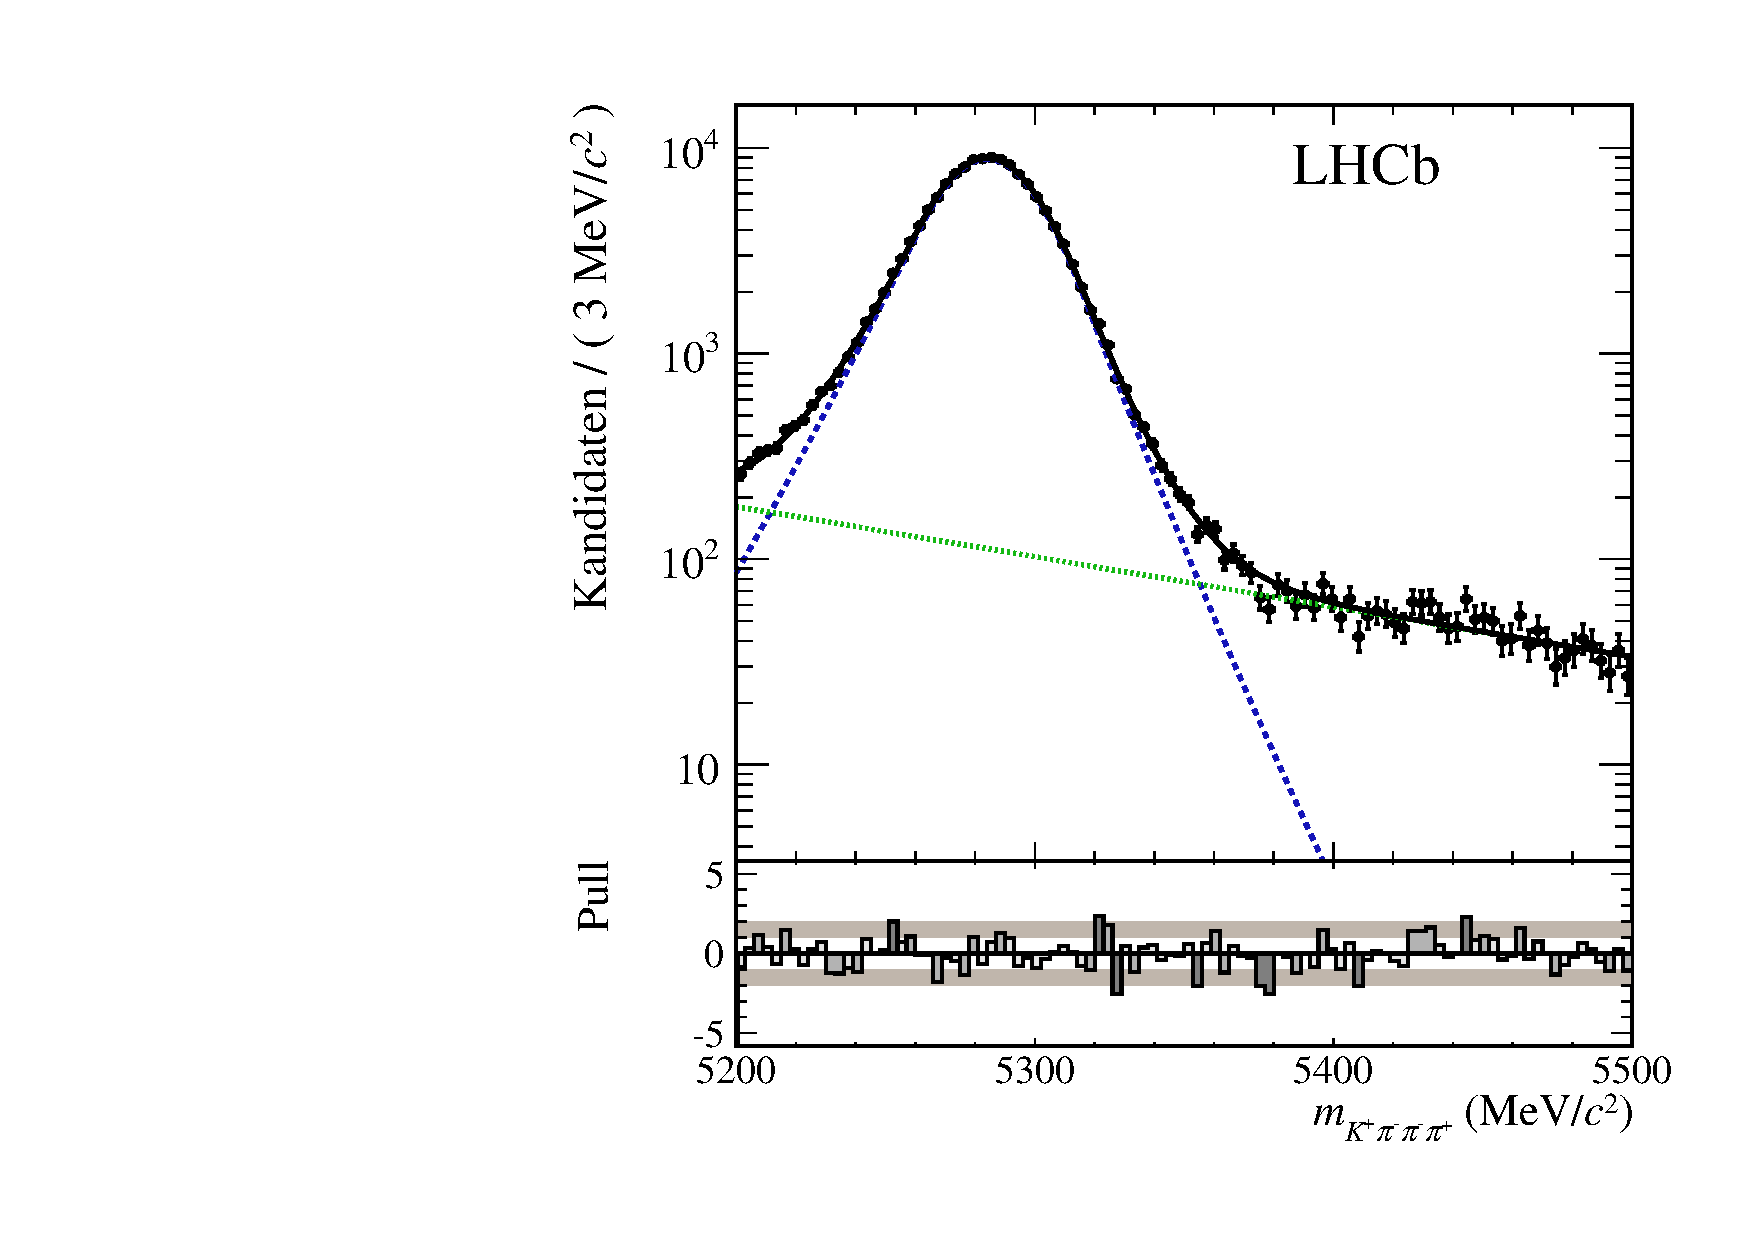
\includegraphics[width=0.49\textwidth]{fig/sweight_2011.pdf}
		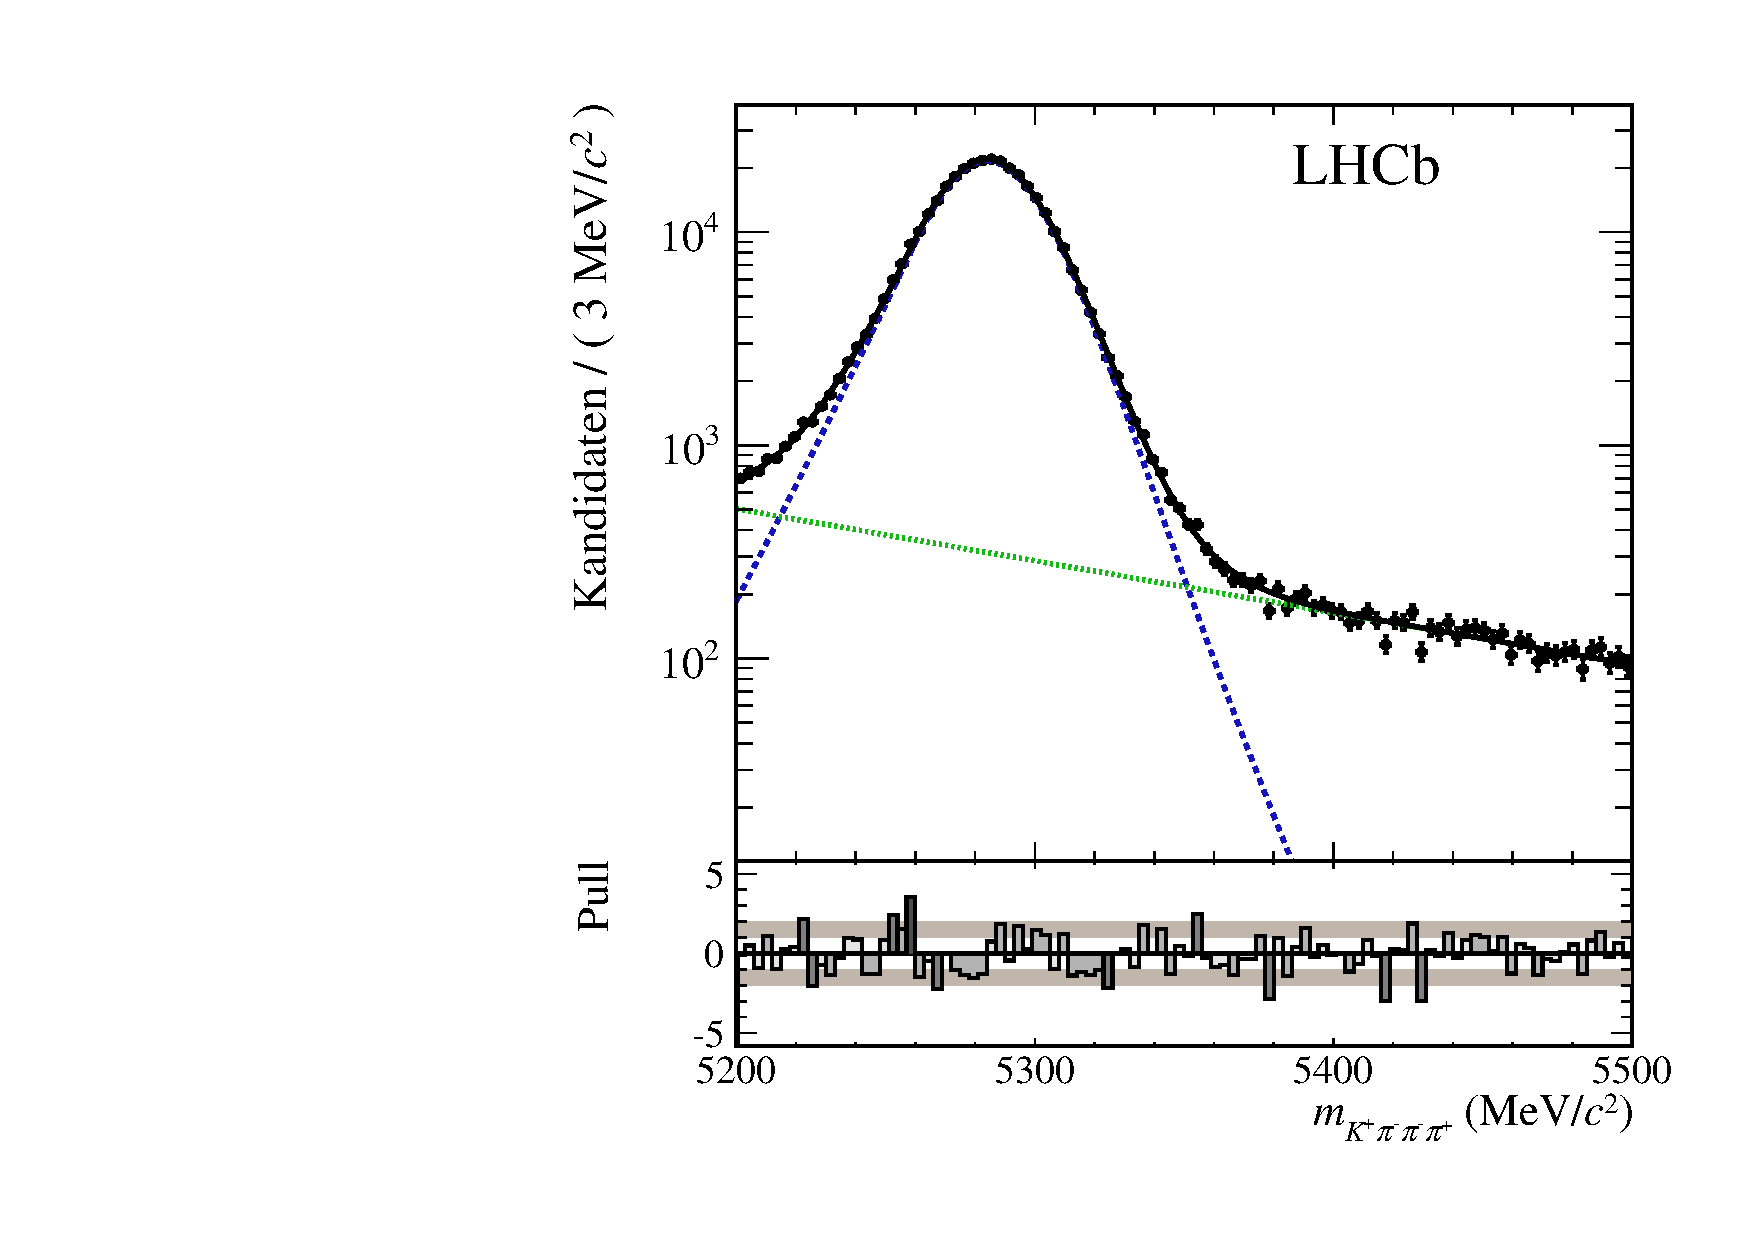
\includegraphics[width=0.49\textwidth]{fig/sweight_2012.pdf}
	\caption{Massenfit zur Bestimmung der Gewichte nach dem \sPlot-Verfahren für Daten des Jahres \num{2011} (links) und \num{2012} (rechts).}
	\label{fig:fit_sweight} 
\end{figure} 

\subsection{Standard OS Kombination}\label{sec:OSkalib}

Da die mistag-Wahrscheinlichkeiten für die OS Kombination eine relativ breite Verteilung haben und nicht eng beieinander liegen, werden für das Jahr \num{2012} zehn und für das Jahr \num{2011} acht Kategorien der mistag-Vorhersage $\eta$ gewählt. Die zehn Kategorien für das Jahr \num{2012}, in denen jeweils Taggingeffizienzen $\varepsilon$ und true-mistag-Wahrscheinlichkeiten $\omega$ durch den Fit ermittelt werden, sind dabei in Abbildung \ref{fig:eta_trennung} zu sehen. 
\begin{figure}[htbp]
	\centering
		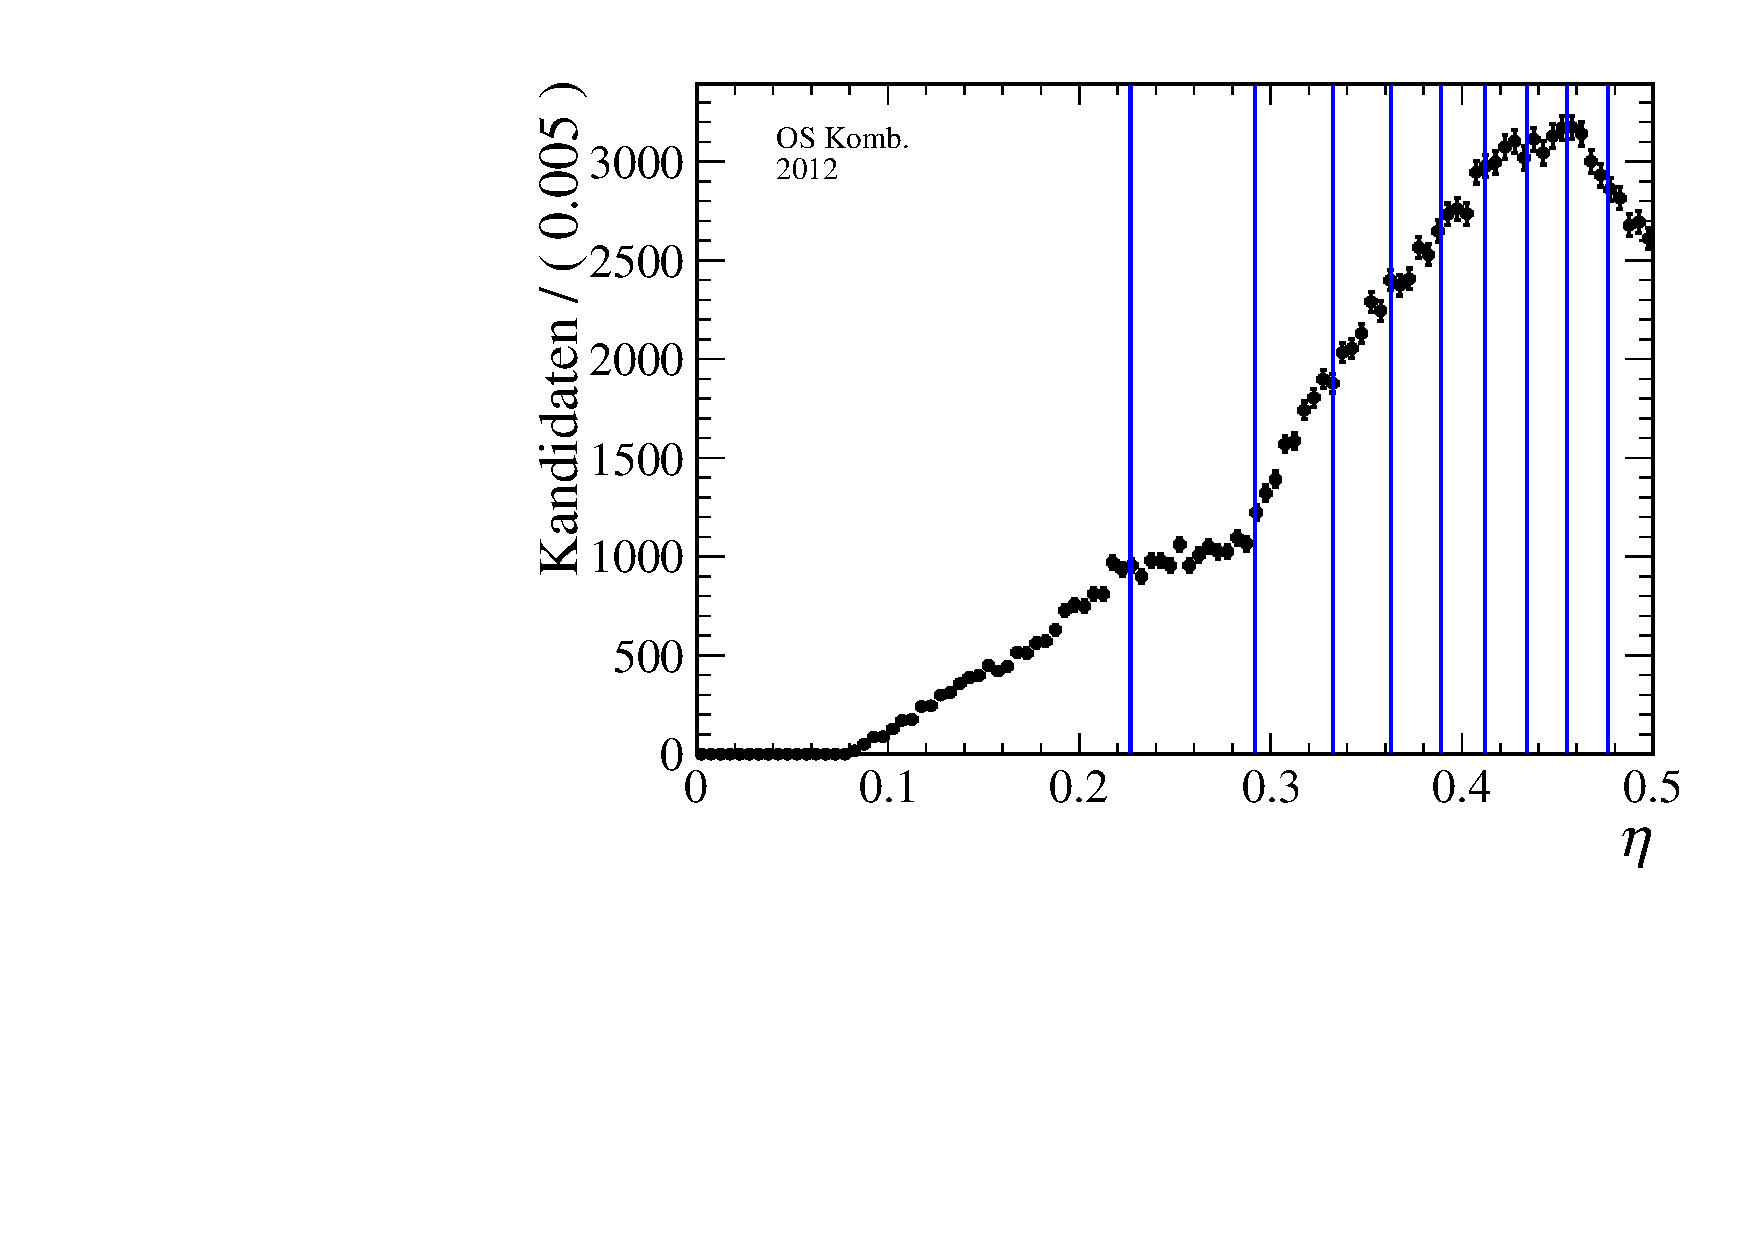
\includegraphics[width=0.75\textwidth]{fig/eta_trennung.pdf}
	\caption{Verteilung der mistag-Wahrscheinlichkeit $\eta$. Die senkrechten blauen Linien zeigen die Trennung in zehn Kategorien mit jeweils gleicher Statistik.}
	\label{fig:eta_trennung} 
\end{figure}
Der zugehörige lineare Fit an die $(\eta,\omega)$-Paare für das Jahr \num{2012} ist in Abbildung \ref{fig:2012_OScomb} zu sehen, die Ergebnisse in Tabelle \ref{tab:result_OScomb}.
\begin{figure}[htbp]
	\centering
		\includegraphics[width=0.75\textwidth]{fig/2012_OScomb.pdf}
	\caption{Fit des linearen Zusammenhangs an die $(\eta,\omega)$-Paare für die Standard OS Kombination auf Daten des Jahres \num{2012} auf dem Kanal \BdToDpi.}
	\label{fig:2012_OScomb} 
\end{figure}
\begin{table}[htbp]
	\centering
	\caption{Ergebnisse der Kalibrierung des OS Kombination für die Jahre \num{2011} und \num{2012} auf dem Kanal \BdToDpi.}
	\label{tab:result_OScomb}
	\begin{tabular}{ccccc}
	\toprule
       Jahr & $\langle\eta\rangle$ & $p_0$ & $\left|p_0-\langle\eta\rangle\right|$ & $p_1$ \\ 
       \midrule 
       2011 & $0{.}365$ & $0{.}369\pm0{.}003$ & $0{.}004$ & $0{.}952\pm0{.}032$ \\
      2012 & $0{.}370$ & $0{.}376\pm0{.}002$ & $0{.}006$ & $0{.}981\pm0{.}020$ \\ 
      \bottomrule
	\end{tabular}
\end{table} 
\begin{table}[htbp]
	\centering
	\caption{Performanz der Standard OS Kombination für das Jahr \num{2012} auf dem Kanal \BdToDpi.}
	\label{tab:2012_OScomb}
	\begin{tabular}{ccccc}
	\toprule
       Kategorie & $\varepsilon(\%)$ & $\omega$ & $D$ & $\varepsilon D^2(\%)$ \\ 
       \midrule
       1 & $3{,}865\pm0{,}035$ & $0{,}186\pm0{,}006$ & $0{,}628\pm0{,}012$ & $1{,}524\pm0{,}060$\\
       2 & $3{,}862\pm0{,}035$ & $0{,}262\pm0{,}006$ & $0{,}476\pm0{,}012$ & $0{,}875\pm0{,}045$\\ 
       3 & $3{,}832\pm0{,}035$ & $0{,}327\pm0{,}006$ & $0{,}346\pm0{,}012$ & $0{,}459\pm0{,}032$\\ 
       4 & $3{,}837\pm0{,}035$ & $0{,}360\pm0{,}006$ & $0{,}280\pm0{,}012$ & $0{,}301\pm0{,}026$\\ 
       5 & $3{,}810\pm0{,}035$ & $0{,}393\pm0{,}006$ & $0{,}214\pm0{,}012$ & $0{,}174\pm0{,}020$\\ 
       6 & $3{,}841\pm0{,}035$ & $0{,}411\pm0{,}006$ & $0{,}178\pm0{,}012$ & $0{,}122\pm0{,}016$\\ 
       7 & $3{,}842\pm0{,}035$ & $0{,}428\pm0{,}006$ & $0{,}144\pm0{,}012$ & $0{,}080\pm0{,}013$\\ 
       8 & $3{,}826\pm0{,}035$ & $0{,}449\pm0{,}006$ & $0{,}102\pm0{,}012$ & $0{,}040\pm0{,}009$\\ 
       9 & $3{,}823\pm0{,}035$ & $0{,}464\pm0{,}006$ & $0{,}072\pm0{,}012$ & $0{,}020\pm0{,}007$\\ 
      10 & $3{,}828\pm0{,}035$ & $0{,}486\pm0{,}006$ & $0{,}028\pm0{,}012$ & $0{,}003\pm0{,}003$\\ 
      \midrule
   Total & $38{,}366\pm0{,}112$& $0{,}377\pm0{,}002$ & $0{,}247\pm0{,}004$ & $3{,}597\pm0{,}091$\\ 
   \bottomrule
	\end{tabular}
\end{table}
Man erkennt zunächst, dass der Parameter $p_0$ um \num{3} Standardabweichungen von dem erwarteten $\langle\eta\rangle$ abweicht, der Parameter $p_1$ stimmt im Rahmen seiner Ungenauigkeit gut mit eins überein. Die Datenpunkte bestätigen allerdings die Annahme eines linearen Zusammenhangs zwischen der mistag-Wahrscheinlichkeit $\eta$ und dem true-mistag $\omega$. 
\begin{figure}[htbp]
	\centering
		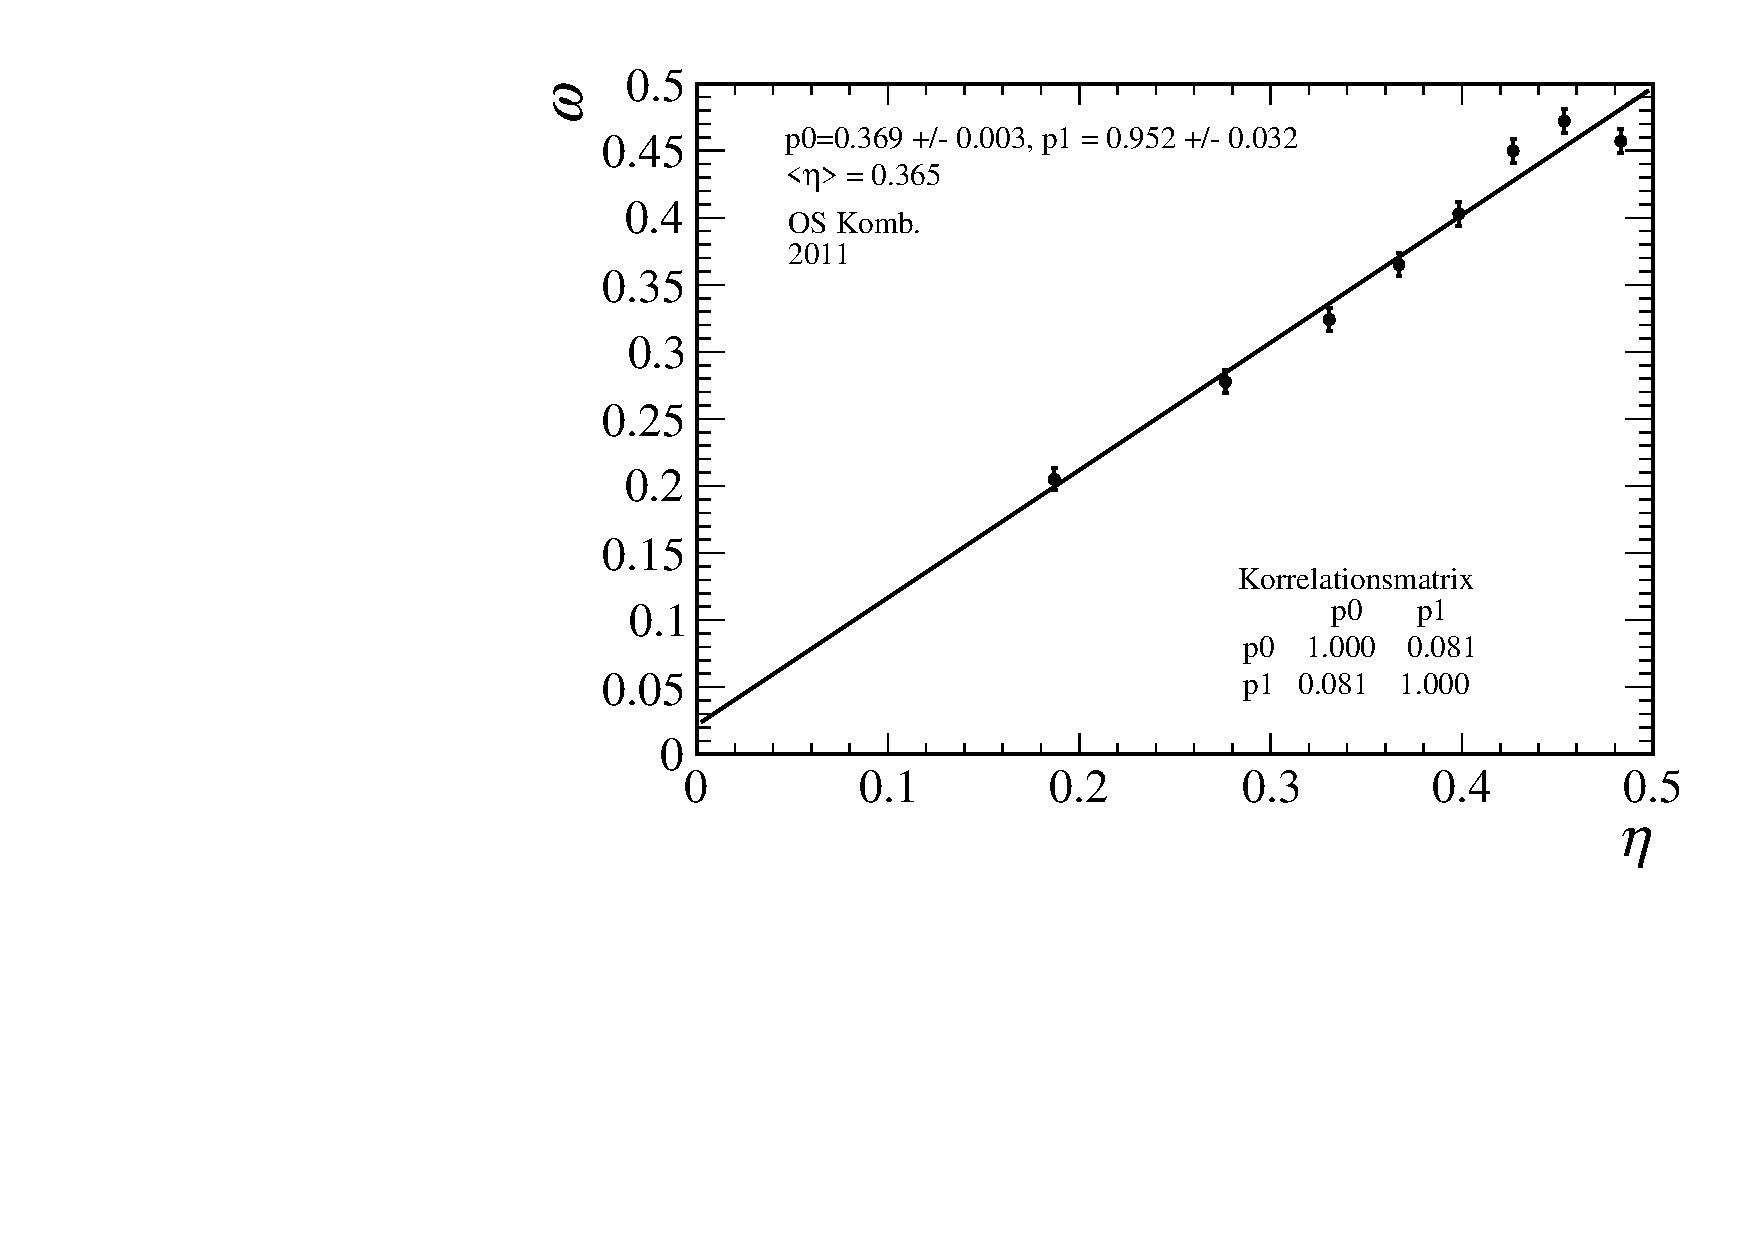
\includegraphics[width=0.75\textwidth]{fig/2011_OScomb.pdf}
	\caption{Fit des linearen Zusammenhangs an die $(\eta,\omega)$-Paare für die Standard OS Kombination auf Daten des Jahres \num{2011} auf dem Kanal \BdToDpi.}
	\label{fig:2011_OScomb} 
\end{figure} 
\begin{table}[htbp]
	\centering
	\caption{Performanz der Standard OS Kombination für das Jahr \num{2011} auf dem Kanal \BdToDpi.}
	\label{tab:2011_OScomb}
	\begin{tabular}{ccccc}
	\toprule
       Kategorie & $\varepsilon(\%)$ & $\omega$ & $D$ & $\varepsilon D^2(\%)$ \\ 
       \midrule 
       1 & $4{,}739\pm0{,}291$ & $0{,}205\pm0{,}008$ & $0{,}590\pm0{,}016$ & $1{,}650\pm0{,}135$\\
       2 & $4{,}723\pm0{,}290$ & $0{,}277\pm0{,}008$ & $0{,}446\pm0{,}016$ & $0{,}939\pm0{,}089$\\ 
       3 & $4{,}652\pm0{,}286$ & $0{,}324\pm0{,}008$ & $0{,}352\pm0{,}016$ & $0{,}576\pm0{,}063$\\ 
       4 & $4{,}664\pm0{,}287$ & $0{,}365\pm0{,}008$ & $0{,}270\pm0{,}016$ & $0{,}340\pm0{,}045$\\ 
       5 & $4{,}650\pm0{,}286$ & $0{,}403\pm0{,}008$ & $0{,}194\pm0{,}016$ & $0{,}175\pm0{,}031$\\ 
       6 & $4{,}673\pm0{,}287$ & $0{,}450\pm0{,}008$ & $0{,}100\pm0{,}016$ & $0{,}047\pm0{,}015$\\ 
       7 & $4{,}673\pm0{,}287$ & $0{,}472\pm0{,}008$ & $0{,}056\pm0{,}016$ & $0{,}015\pm0{,}008$\\ 
       8 & $4{,}675\pm0{,}288$ & $0{,}457\pm0{,}008$ & $0{,}086\pm0{,}016$ & $0{,}035\pm0{,}013$\\ 
       \midrule
   Total & $37{,}449\pm0{,}814$& $0{,}369\pm0{,}003$ & $0{,}262\pm0{,}006$ & $3{,}777\pm0{,}183$\\ 
   \bottomrule
	\end{tabular}
\end{table}
Die Ergebnisse des Jahres \num{2011} sind in der Abbildung \ref{fig:2011_OScomb}  und in der Tabelle \ref{tab:result_OScomb} zu sehen. Hier stimmen beide Parameter im Fit zufriedenstellend mit ihren Erwartungen überein. Ebenso ist der lineare Zusammenhang in den Datenpunkten gut erkennbar.\\
Die Ergebnisse für die Taggingeffizienzen $\varepsilon$ und effektiven Taggingeffizienzen $\varepsilon D^2$ für beide Jahre sind in den Tabellen \ref{tab:2012_OScomb} und \ref{tab:2011_OScomb} zu sehen. Dabei sieht man hier jeweils die Einzelergebnisse für die verschiedenen Kategorien der mistag-Wahrscheinlichkeit $\eta$. Man beobachtet, dass, obwohl alle Kategorien eine nahezu identische Statistik beitragen, die ersten Kategorien, aufgrund ihrer kleinen Werte für $\omega$ am stärksten zu effektiven Taggingeffizienz $\epsilon D^2$ beitragen. Die höheren Kategorien tragen mit größer werdenden true-mistag-Wahrscheinlichkeiten dann immer weniger zur gesamten effektiven Taggingeffizienz $\varepsilon D^2$ bei. Insgesamt sind die Ergebnisse der Taggingeffizienzen für beide Jahre vergleichbar und die Tagger können als kalibriert angesehen werden. Die Abweichung für das Jahr \num{2012} resultiert dabei aus der Tatsache, dass die Kalibrierung an dieser Stelle aus dem Zerfallskanal \BuToJPsiKp stammt und daher experimentell durchaus Unterschiede in den Kalibrierungsparametern $p_0$ und $p_1$ zu erwarten sind. Weiter sind an dieser Stelle noch keine systematischen Unsicherheiten berücksichtigt. 

\subsection{Der OS Charm Tagger}

Für den OS Charm Tagger erhält man im Jahr \num{2011} eine Taggingeffizienz von $\varepsilon=\SI{3{,}264}{\%}$ und für das Jahr \num{2012} von $\varepsilon=\SI{3{,}304}{\%}$ . Aufgrund der in beiden Jahren relativ geringen Statistik wurde eine minimale Anzahl von fünf Kategorien gewählt, um eine ausreichende Anzahl Datenpunkte für den linearen Fit zu behalten. Die Ergebnisse der linearen Fits sind in Abbildung \ref{fig:fit_OSCharm} und in Tabelle \ref{tab:result_OSCharm} zu sehen.
\begin{figure}[htbp]
	\centering
		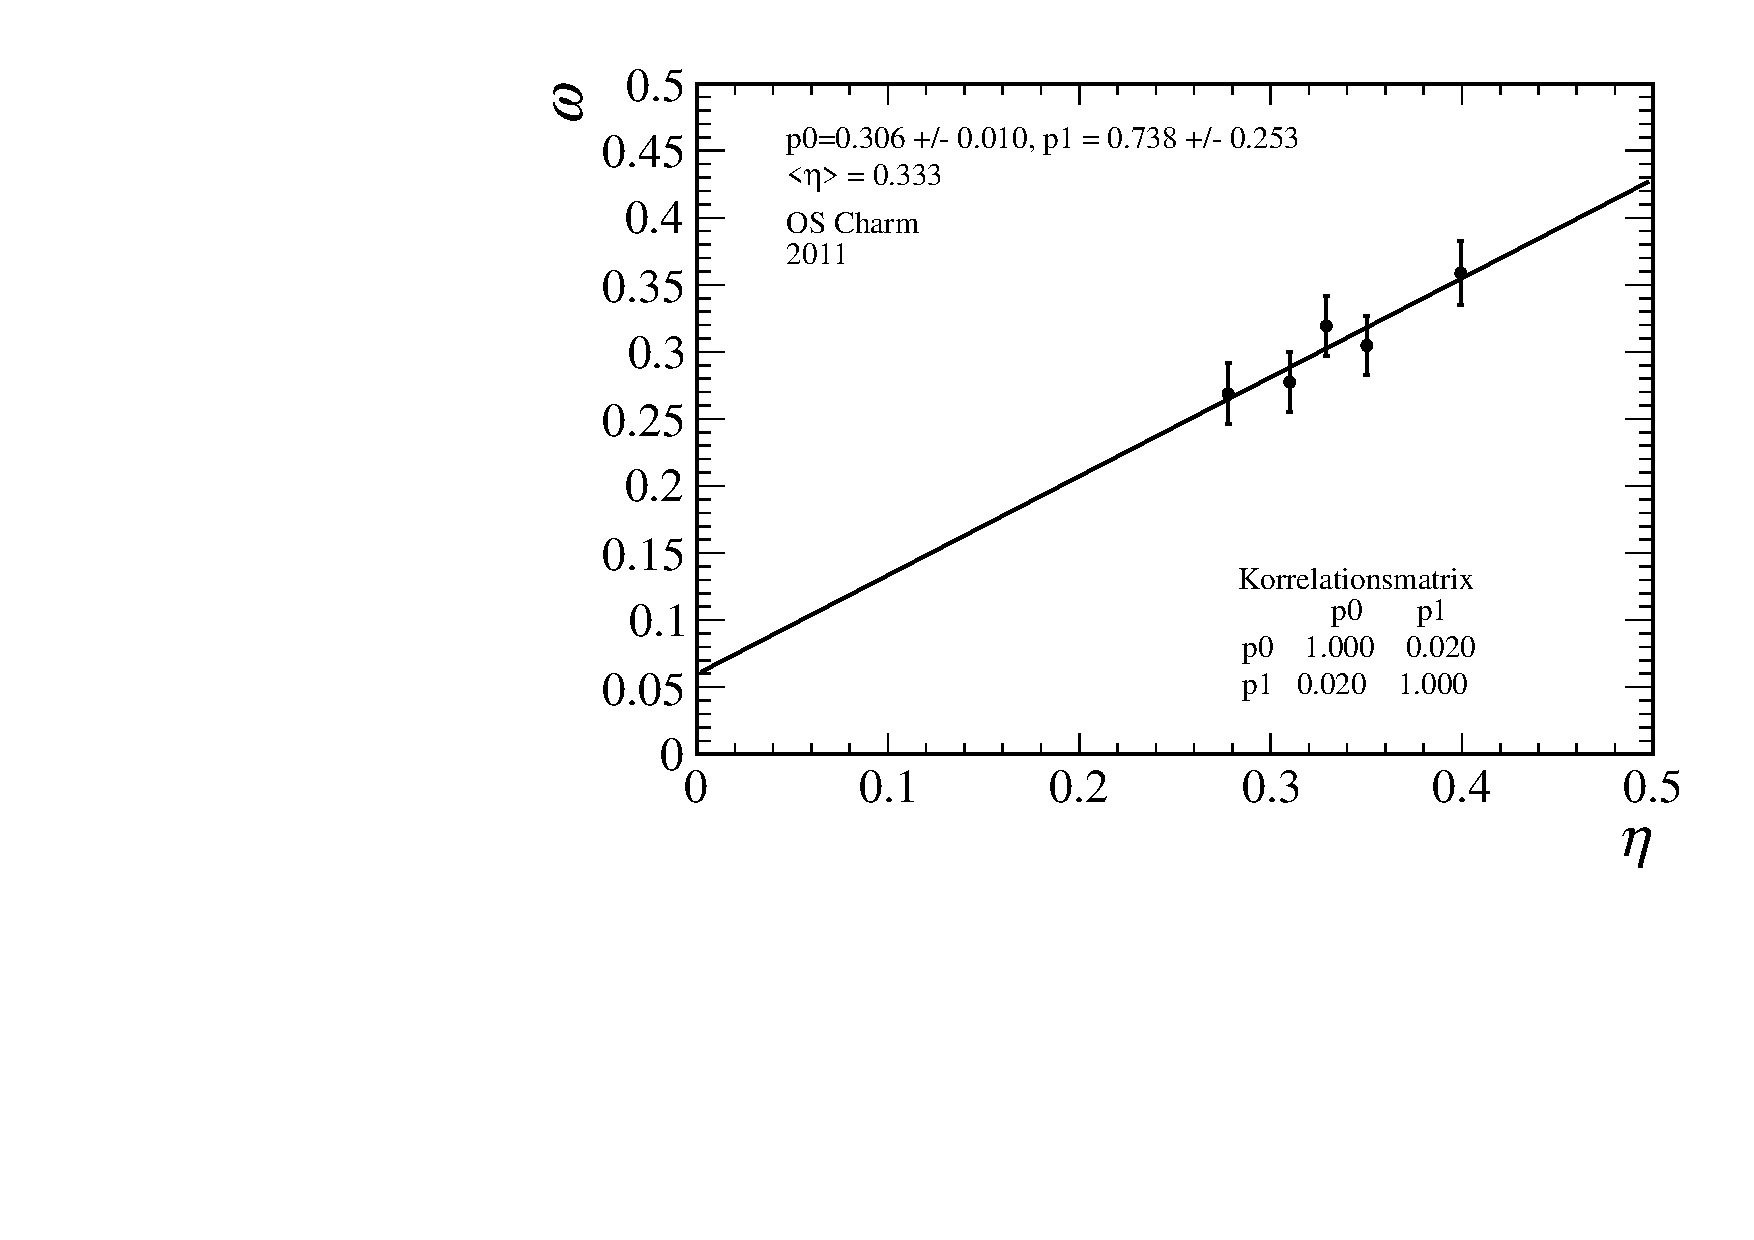
\includegraphics[width=0.49\textwidth]{fig/2011_OSCharm.pdf}
		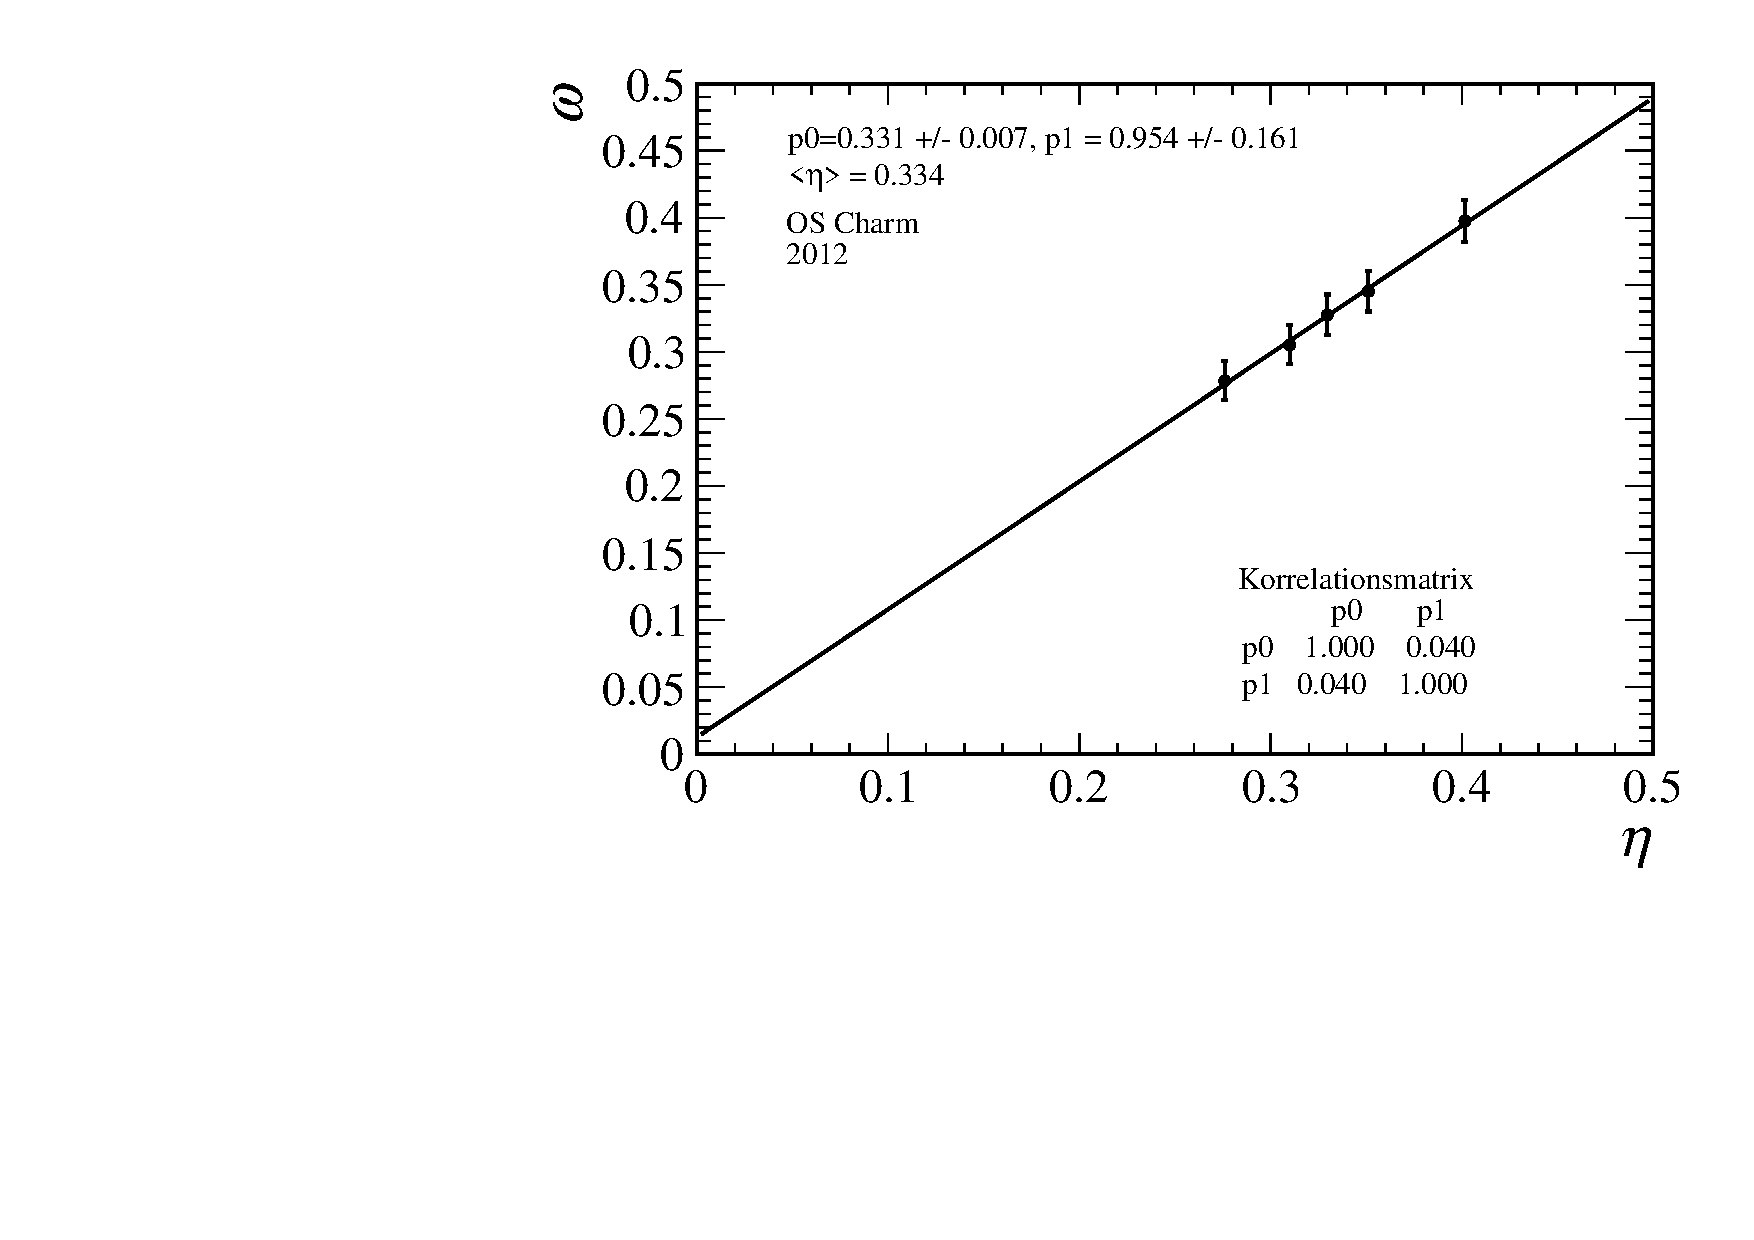
\includegraphics[width=0.49\textwidth]{fig/2012_OSCharm.pdf}
	\caption{Fit des linearen Zusammenhangs an die $(\eta,\omega)$-Paare für den OS Charm Tagger auf Daten des Jahres \num{2011} (links) und \num{2012} (rechts) auf dem Kanal \BdToDpi.}
	\label{fig:fit_OSCharm} 
\end{figure} 
Für das Jahr \num{2012} liegen beide Parameter des linearen Fits innerhalb einer Standardabweichung in der Erwartungen an eine ideale Kalibration und die Datenpunkte passen zur Hypothese eines linearen Zusammenhangs, sodass der Tagger hier als kalibiert angesehen werden kann. 
\begin{table}[htbp]
	\centering
	\caption{Ergebnisse der Kalibrierung des OS Charm Taggers für die Jahre \num{2011} und \num{2012} auf dem Kanal \BdToDpi.}
	\label{tab:result_OSCharm}
	\begin{tabular}{ccccc}
	\toprule
       Jahr & $\langle\eta\rangle$ & $p_0$ & $\left|p_0-\langle\eta\rangle\right|$ & $p_1$ \\ 
       \midrule
       2011 & $0{.}333$ & $0{.}306\pm0{.}010$ & $0{.}027$ & $0{.}738\pm0{.}253$ \\
      2012 & $0{.}334$ & $0{.}331\pm0{.}007$ & $0{.}003$ & $0{.}954\pm0{.}161$ \\ 
      \bottomrule
	\end{tabular}
\end{table}
\begin{table}[htbp]
	\centering
	\caption{Performanz des OS Charm Taggers für die Jahre \num{2011} und \num{2012} auf dem Kanal \BdToDpi.}
	\label{tab:performance_OSCharm}
	\begin{tabular}{ccccc}
	\toprule
       Jahr & $\varepsilon(\%)$ & $\omega$ & $D$ & $\varepsilon D^2(\%)$ \\ 
       \midrule
      2011 & $3{,}304\pm0{,}102$ & $0{,}306\pm0{,}010$ & $0{,}388\pm0{,}020$ & $0{,}512\pm0{,}049$\\ 
   2012 & $3{,}264\pm0{,}032$ & $0{,}331\pm0{,}007$ & $0{,}338\pm0{,}014$ & $0{,}395\pm0{,}041$\\ 
   \bottomrule
  \end{tabular}
\end{table}
Die Ergebnisse für das Jahr \num{2011} zeigen eine etwas schlechtere Linearität der $(\eta,\omega)$-Paare, außerdem weicht der Parameter $p_0$ um \num{2{,}7} Standardabweichungen von dem erwarteten $\langle\eta\rangle$ ab.\\
Die Taggingeffizienzen $\varepsilon$ und die effektiven Taggingeffizienzen $\varepsilon D^2$  (Tabelle \ref{tab:performance_OSCharm}) sind für das Jahr \num{2011} in beiden Jahren etwas höher. Insgesamt kann auch hier der Tagger für beide Jahre als kalibriert angesehen werden, die Abweichung für den Parameter $p_0$ für das Jahr \num{2011} resultieren dabei wieder aus einer Kalibrierung in einem anderen Zerfallskanal.\\
Weiterhin wird hier bestätigt, dass der OS Charm Tagger eine geringe Anzahl an getaggten Ereignisse aufweist, jedoch ebenso kleine mistag-Vorhersagen $\omega$ ausgibt. Somit ergibt sich, vor allem wegen der sehr kleinen Taggingeffizienzen $\varepsilon$, eine kleine effektive Taggingeffizienz $\varepsilon D^2$. 

\subsection{Der OS Kaon nnet Tagger}

Ebenso wie bei dem OS Charm Tagger handelt es sich bei dem OS Kaon nnet Tagger um eine Neuentwicklung. Allerdings liefert der OS Kaon nnet Tagger vergleichsweise große Anzahlen an getaggten Ereignissen mit großen mistag-Vorhersagen $\eta$. Für das Jahr \num{2011} erhält man in $\Bz\rightarrow\Dp\pim$ Taggingeffizienzen von $\varepsilon=\SI{45{,}044}{\%}$ und für das Jahr \num{2012} vom $\varepsilon=\SI{46{,}459}{\%}$. Da die mistag-Wahrscheinlichkeiten jedoch bei Werten $>\num{0{,}4}$ liegen (Abbildung \ref{fig:eta_oskaon}), werden trotz der hohen Ereigniszahlen weniger Kategorien als beispielsweise für die OS Standard Kombination gewählt. 
\begin{figure}[htbp]
	\centering
		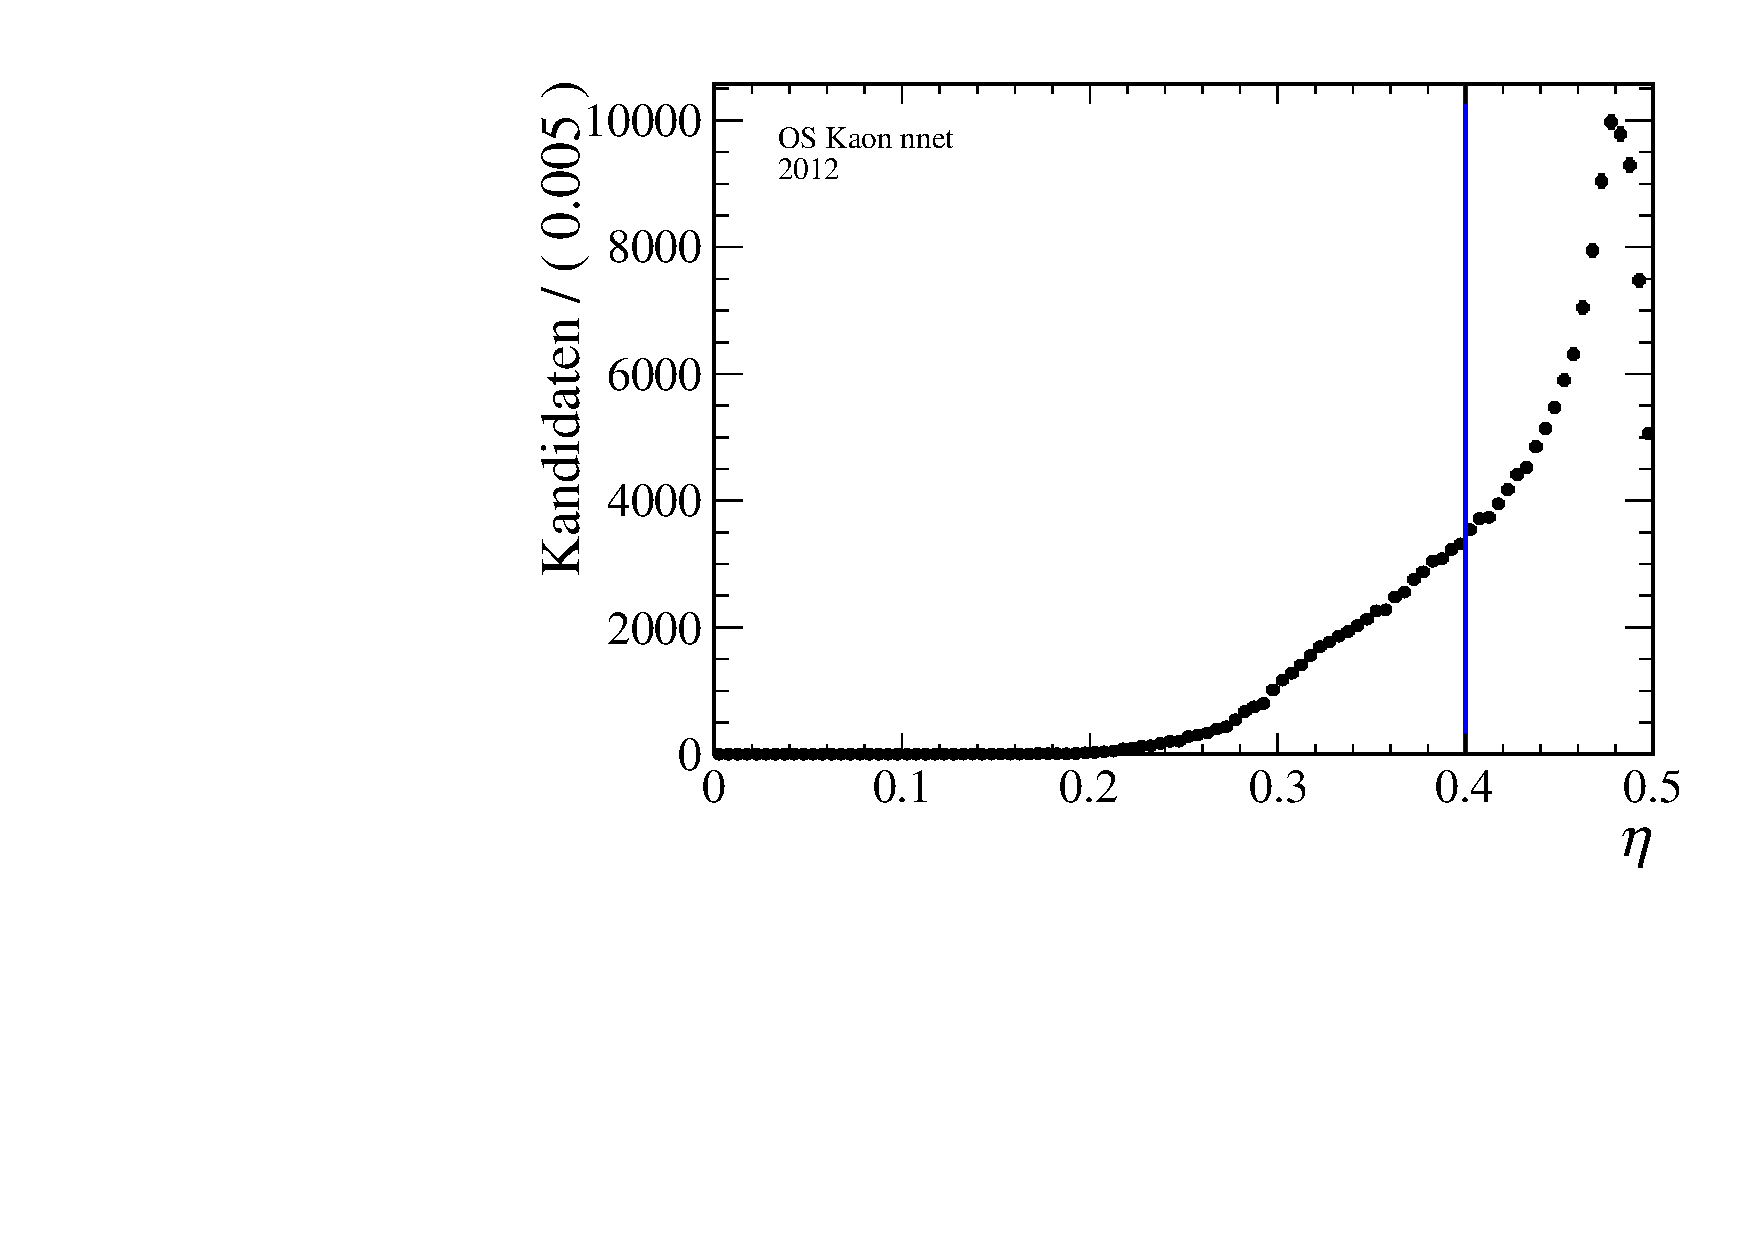
\includegraphics[width=0.75\textwidth]{fig/Eta_OSKaon.pdf}
	\caption{Verteilung der mistag-Wahrscheinlichkeit $\eta$ für den OS Kaon nnet Tagger für das Jahr \num{2012}. Man sieht, dass die meisten Kandidaten $\eta$-Werte über \num{0{,}4} (blaue senkrechte Linie) haben.}
	\label{fig:eta_oskaon} 
\end{figure} 
Die Ergebnisse der linearen Fits sind in Abbildung \ref{fig:fit_OSKaonNN} und Tabelle \ref{tab:result_OSKaonNN} zu sehen.
\begin{figure}[htbp]
	\centering
		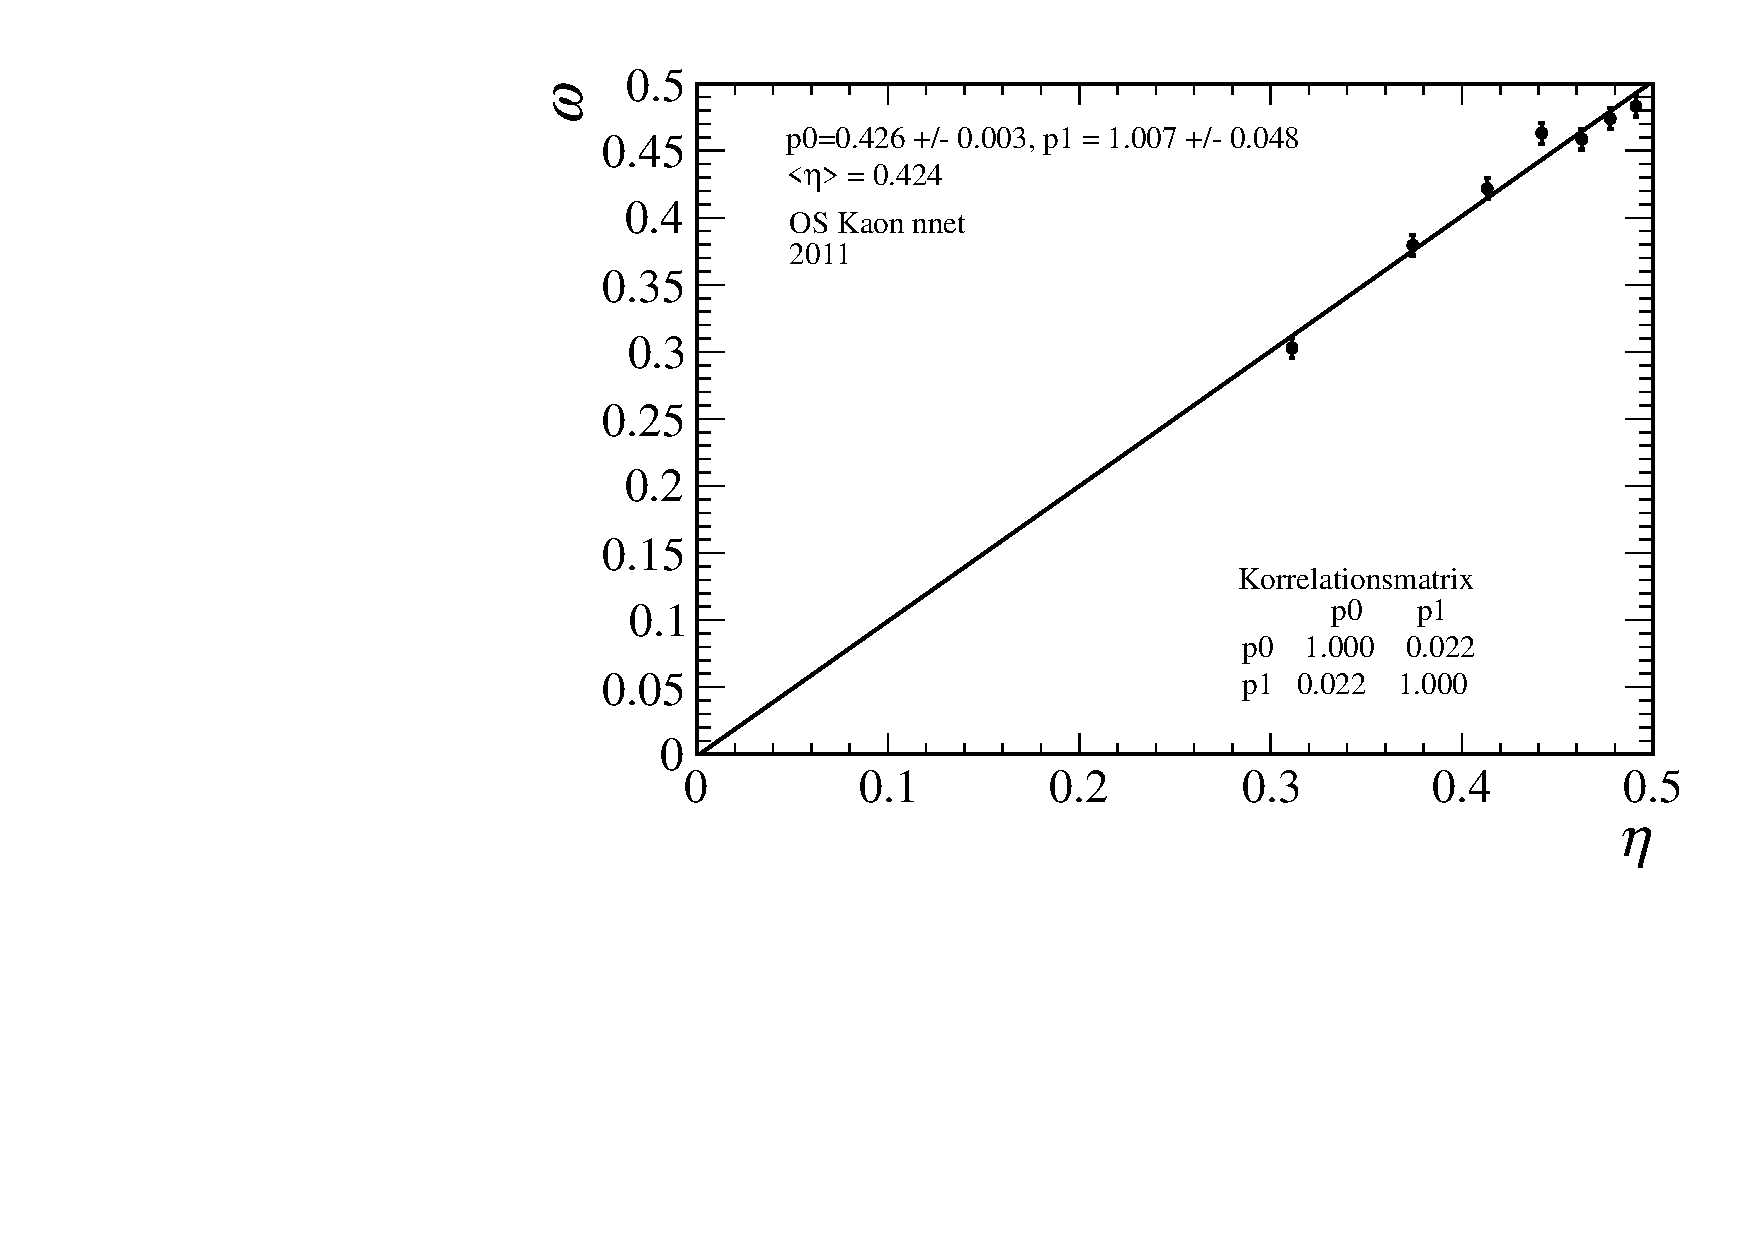
\includegraphics[width=0.49\textwidth]{fig/2011_OSKaonNN.pdf}
		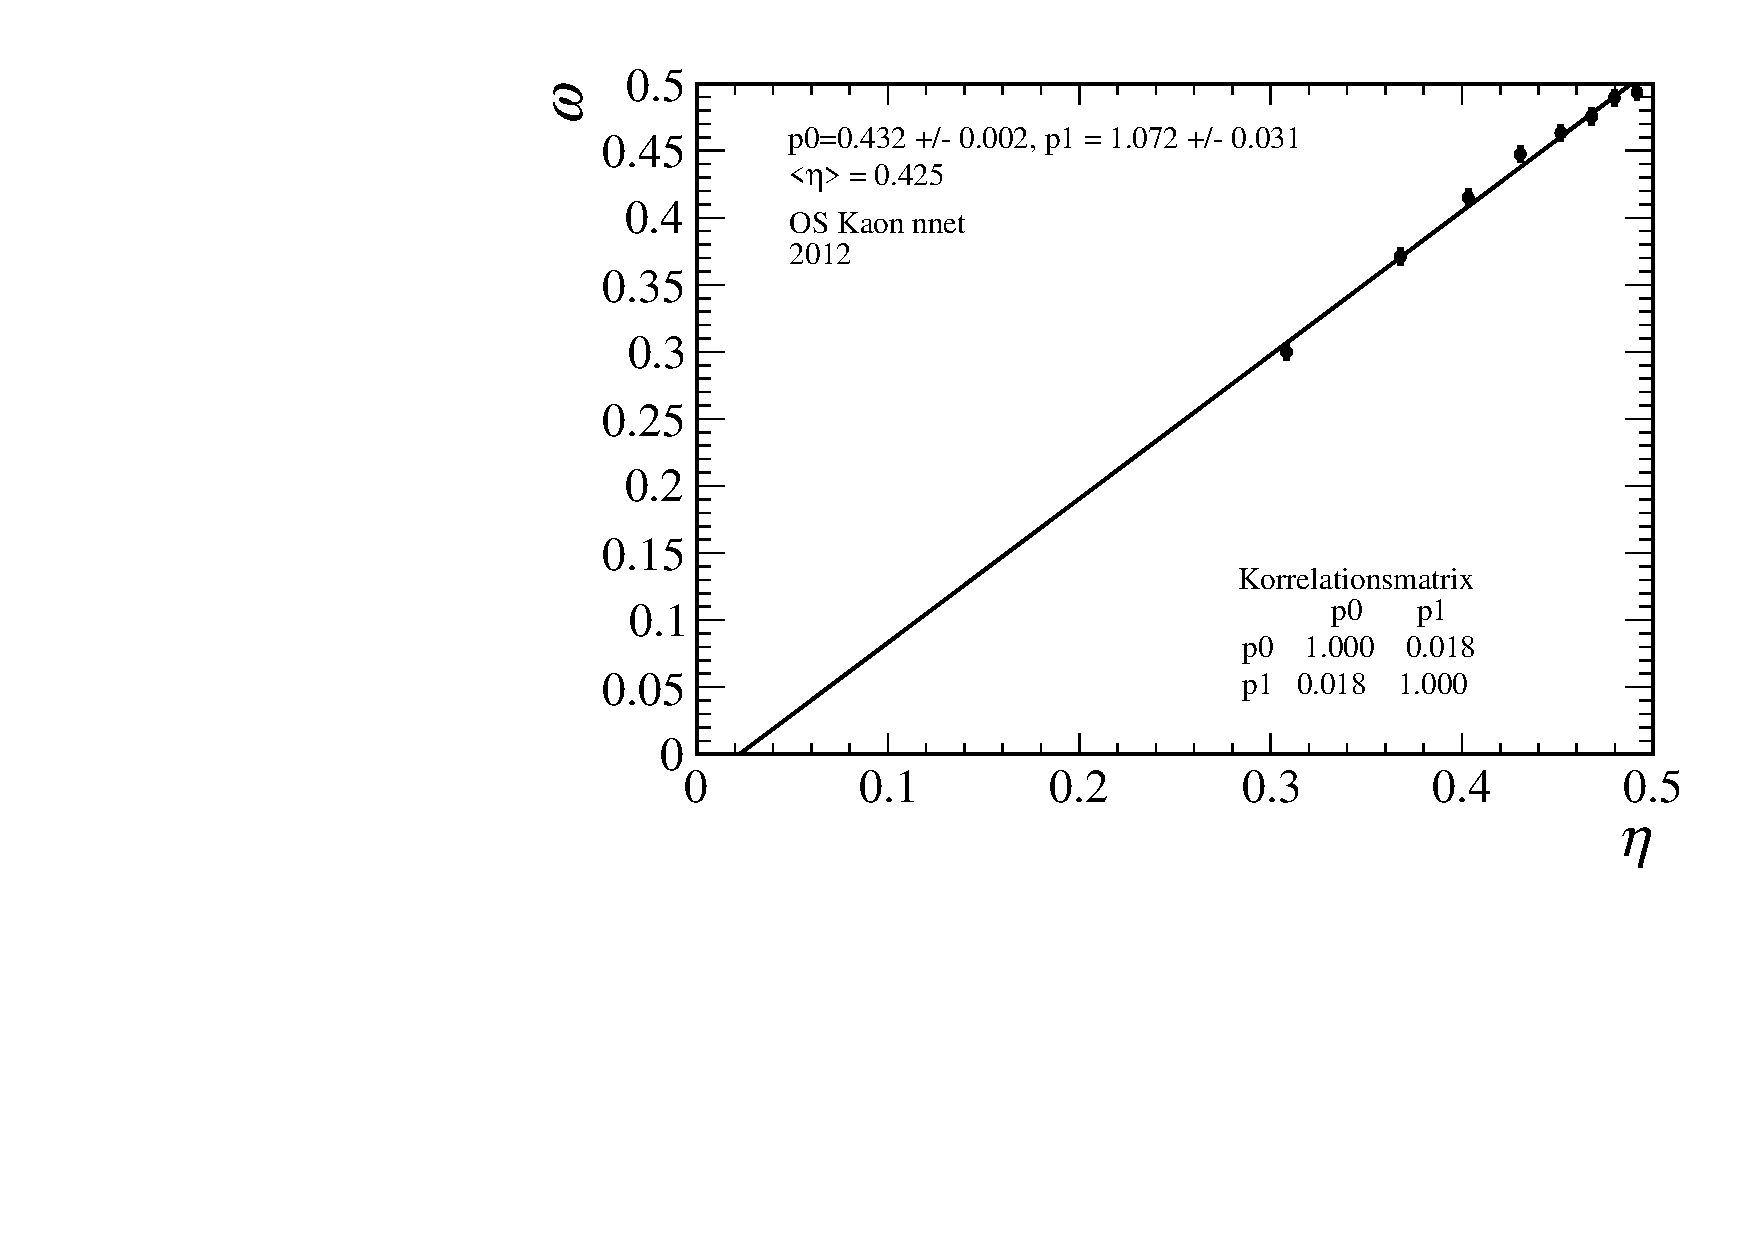
\includegraphics[width=0.49\textwidth]{fig/2012_OSKaonNN.pdf}
	\caption{Fit des linearen Zusammenhangs an die $(\eta,\omega)$-Paare für den OS Kaon nnet Tagger auf Daten des Jahres \num{2011} (links) und \num{2012} (rechts) auf dem Kanal \mbox{\BdToDpi}.}
	\label{fig:fit_OSKaonNN} 
\end{figure} 
Wie bei der Standard OS Kombination, ist auch hier zu sehen, dass die Kalibrierung für das Jahr \num{2012} nicht optimal ist. Beide Parameter $p_0$ und $p_1$ weichen um mehr als \num{2} Standardabweichungen von ihren Erwartungen ab. Auch hier wird der lineare Zusammenhang zwischen der vorhergesagten mistag-Wahrscheinlichkeit $\eta$ und dem true-mistag $\omega$ bestätigt. Für das Jahr \num{2011} stimmen beide Parameter gut mit ihren Erwartungen überein.  
\begin{table}[htbp]
	\centering
	\caption{Ergebnisse der Kalibrierung des OS Kaon nnet Taggers für die Jahre \num{2011} und \num{2012} auf dem Kanal \BdToDpi.}
	\label{tab:result_OSKaonNN}
	\begin{tabular}{ccccc}
	\toprule
       Jahr & $\langle\eta\rangle$ & $p_0$ & $\left|p_0-\langle\eta\rangle\right|$ & $p_1$ \\ 
       \midrule 
	2011 & $0{.}425$ & $0{.}426\pm0{.}003$ & $0{.}001$ & $1{.}007\pm0{.}048$ \\
   2012 & $0{.}425$ & $0{.}432\pm0{.}002$ & $0{.}007$ & $1{.}073\pm0{.}031$ \\ 
   \bottomrule
	\end{tabular}
\end{table}
\begin{table}[htbp]
	\centering
	\caption{Performanz des OS Kaon nnet für die Jahre \num{2011} und \num{2012} auf dem Kanal \mbox{\BdToDpi}.}
	\label{tab:performance_OSKaonNN}
	\begin{tabular}{ccccc}
	\toprule
       Jahr & $\varepsilon(\%)$ & $\omega$ & $D$ & $\varepsilon D^2(\%)$ \\ 
       \midrule
       2011 & $45{,}044\pm1{,}041$& $0{,}426\pm0{,}003$ & $0{,}147\pm0{,}006$ & $1{,}621\pm0{,}122$\\
     2012 & $46{,}459\pm0{,}125$& $0{,}432\pm0{,}002$ & $0{,}136\pm0{,}004$ & $1{,}588\pm0{,}061$\\ 
     \bottomrule
  \end{tabular}
\end{table}
Die in Tabelle \ref{tab:performance_OSKaonNN} dargestellten Taggingeffizienzen $\varepsilon$ sind für beide Jahre ähnlich, ebenso die effektiven Taggingeffizienz $\varepsilon D^2$. Zusammenfassend lässt sich der Tagger für das Jahr \num{2011} als gut kalibriert bezeichnen, für das Jahr \num{2012} ist diese Aussage schwieriger. Die größeren Abweichungen für das Jahr \num{2012} haben die gleiche Ursache wie bei der Standard OS Kombination. Aus diesem Grund lässt sich für das Jahr \num{2012} sagen, dass der OS Kaon nnet Tagger kalibriert ist, diese Kalibration auf \BdToDpi allerdings nicht ideal ist.   

\section{Kalibrierung der SS Tagger}

Im Weiteren wird nun auf die Kalibrierung der SS Tagger eingegangen. Die Parameter der Zerfallszeitakzeptanz werden dabei ebenfalls wieder in allen Kanälen mit dem zuvor beschriebenen \sPlot-Verfahren \cite{splot} bestimmt (Abbildung \ref{fig:fit_sweight}). Bei der Selektion der Taggingteilchen für die Tagger auf der Same Side wird das Signal mit beeinflusst. Dadurch kommt es in den unterschiedlichen Kategorien der mistag-Verteilung $\eta$ zu Unterschieden, die im Fit berücksichtigt werden müssen.

\subsection{Der SS Pion Tagger}

Der schnittbasierte SS Pion Tagger hat für das Jahr \num{2011} eine Taggingeffizienz von $\varepsilon=\SI{14{,}847}{\%}$ und für das Jahr \num{2012} von $\varepsilon=\SI{15{,}146}{\%}$. Für \num{2011} werden sechs und für \num{2012} sieben $\eta$-Kategorien gewählt. In Abbildung \ref{fig:fit_SSPion} und Tabelle \ref{tab:result_SSPion} sind die Ergebnisse der Kalibrierung für die Jahre \num{2011} und \num{2012} dargestellt.
\begin{figure}[htbp]
	\centering
		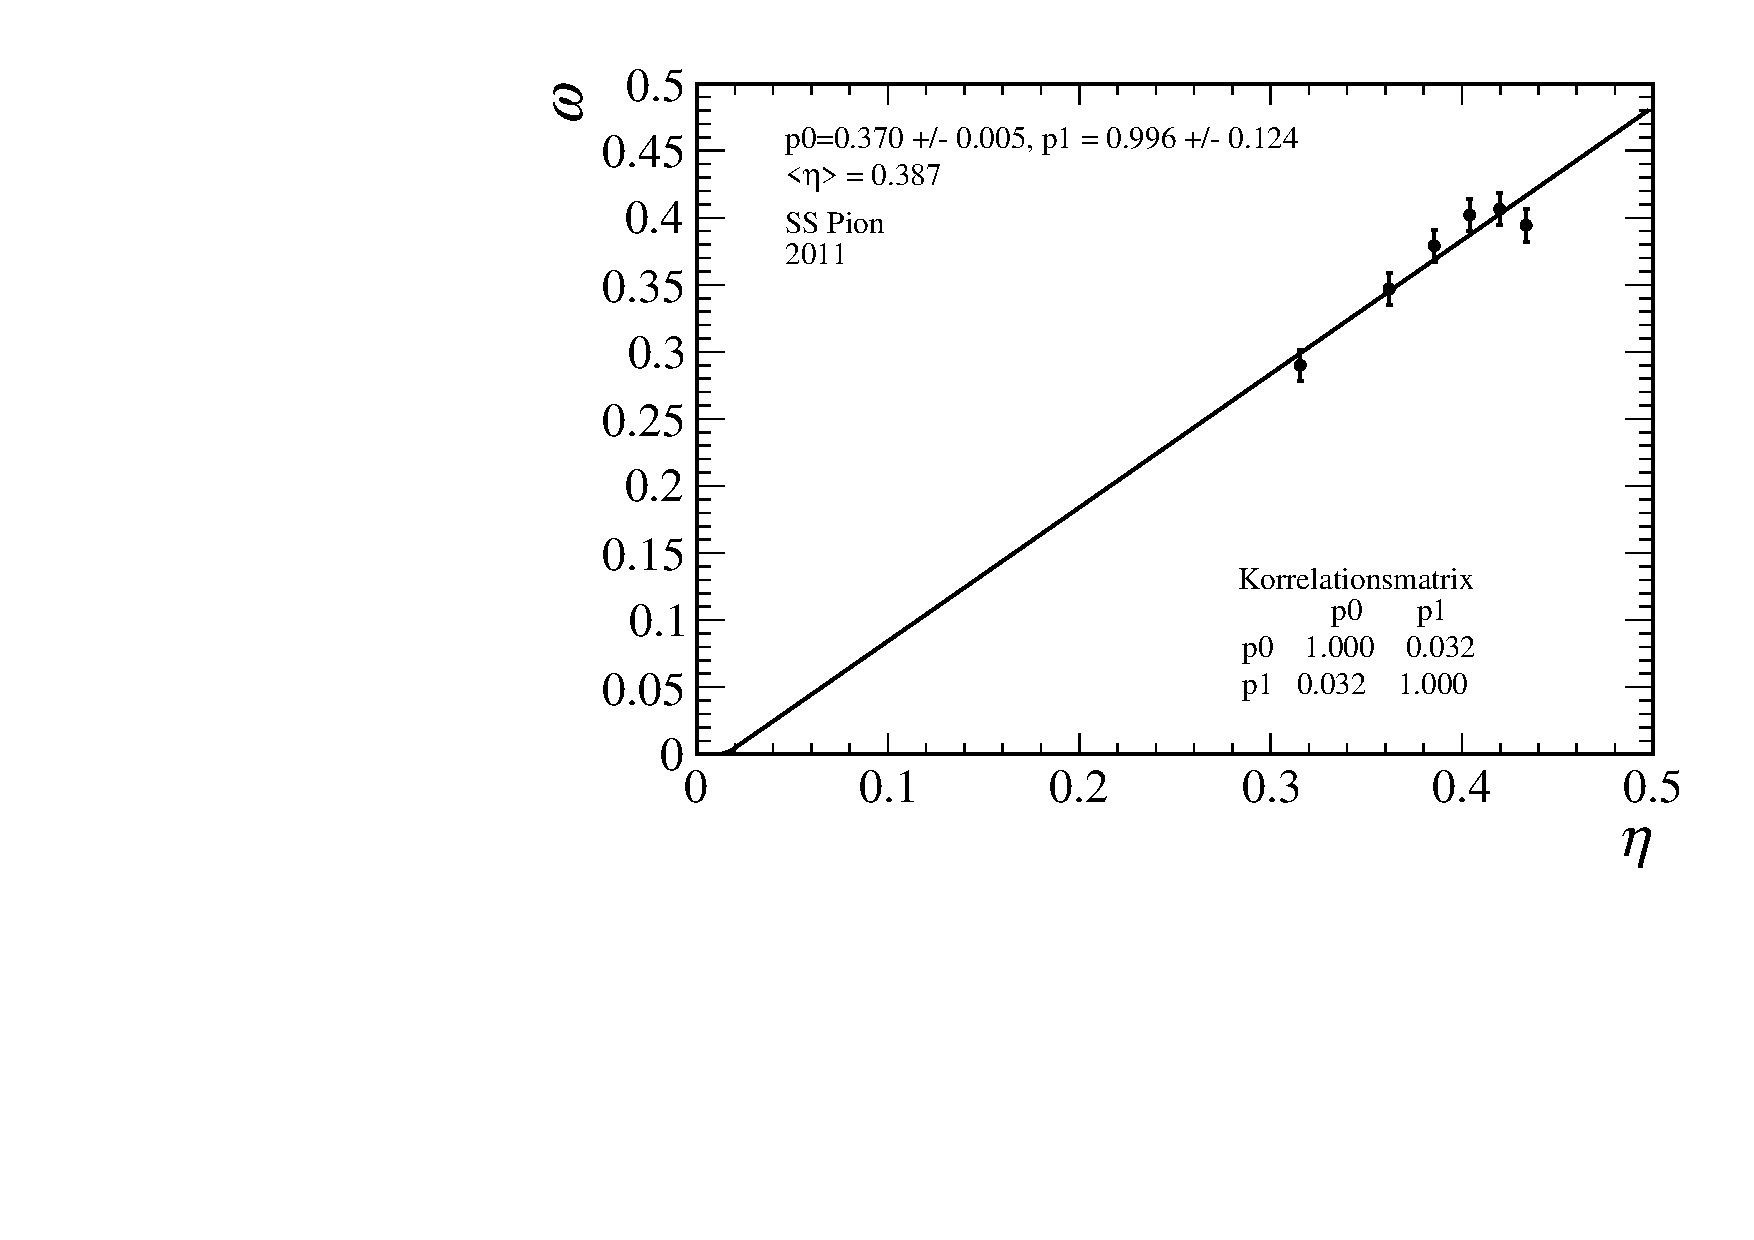
\includegraphics[width=0.49\textwidth]{fig/2011_SSPion.pdf}
		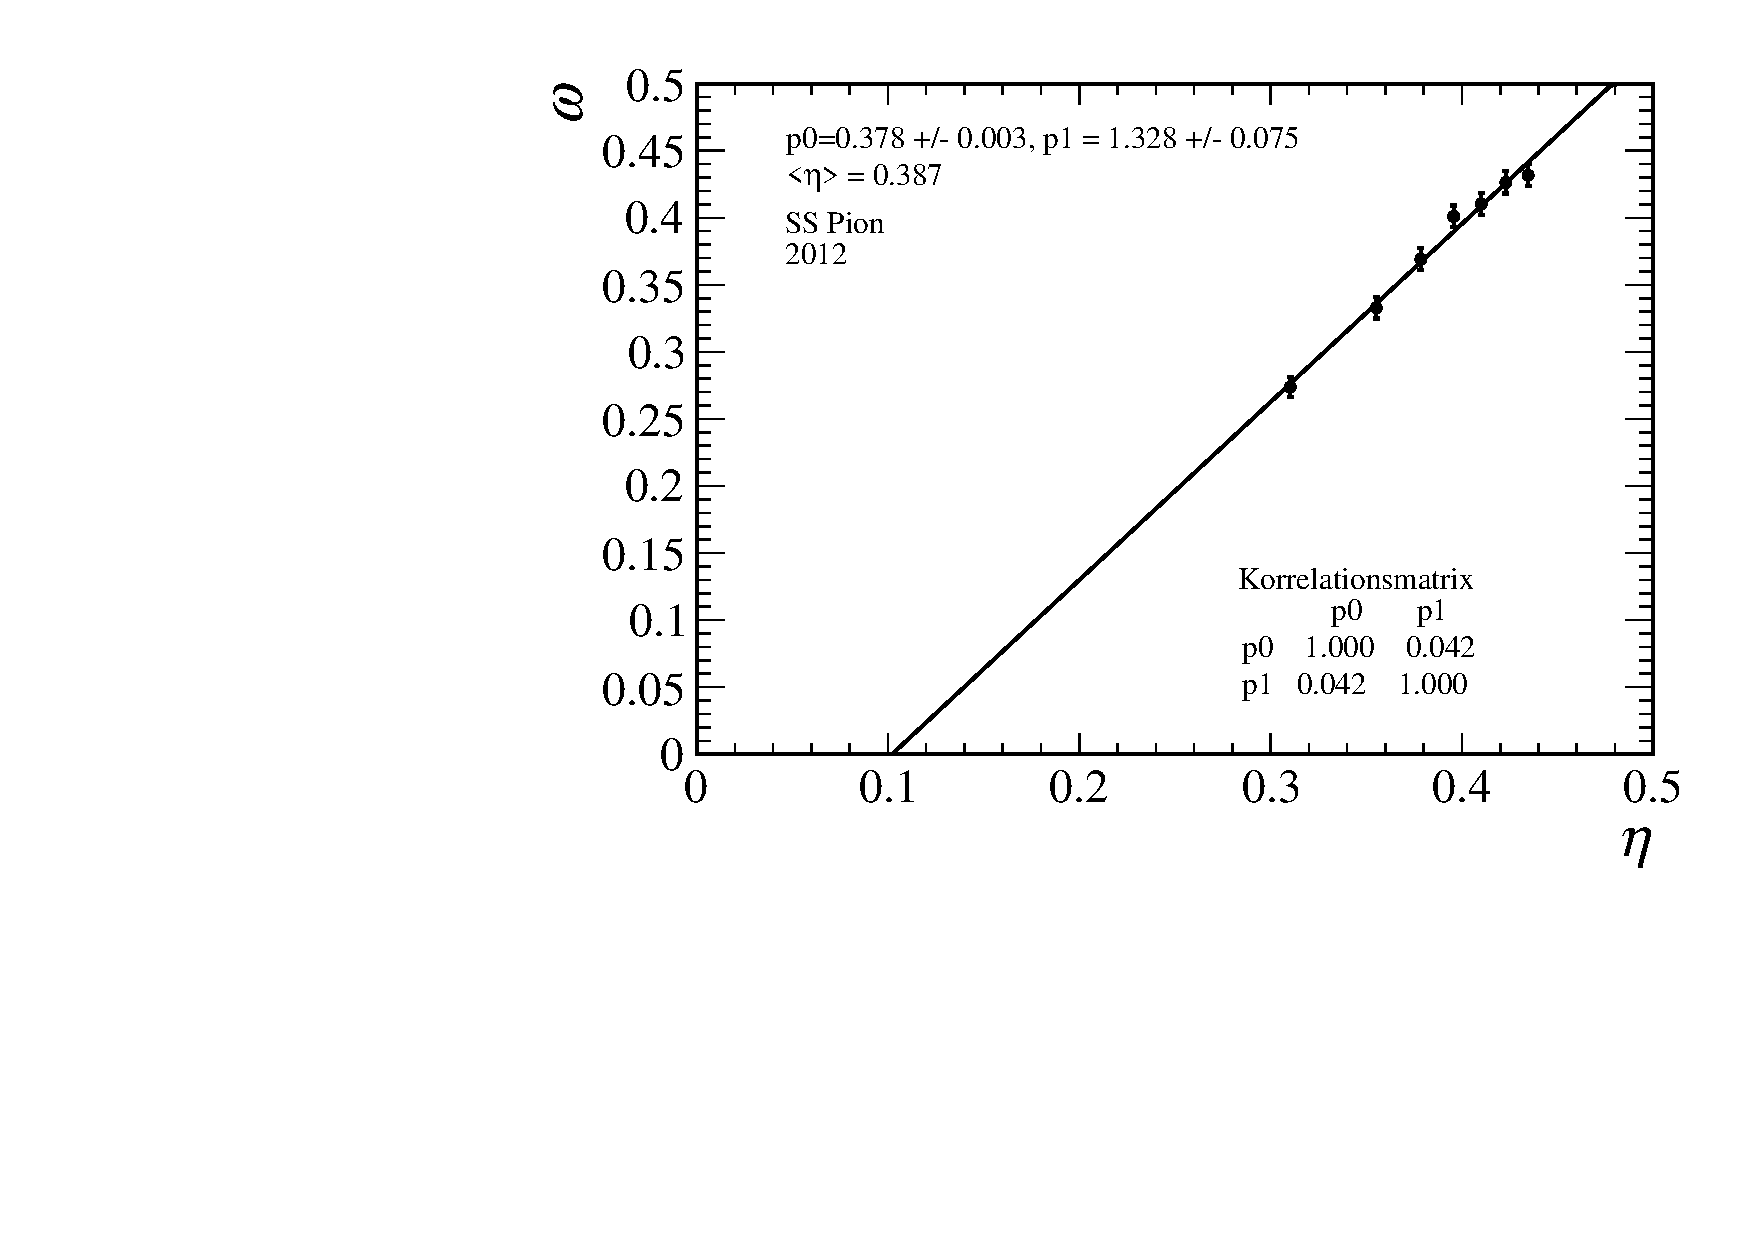
\includegraphics[width=0.49\textwidth]{fig/2012_SSPion.pdf}
	\caption{Fit des linearen Zusammenhangs an die $(\eta,\omega)$-Paare für den SS Pion Tagger auf Daten des Jahres \num{2011} (links) und \num{2012} (rechts) auf dem Kanal \BdToDpi.}
	\label{fig:fit_SSPion} 
\end{figure}
Für das Jahr \num{2012} wird deutlich, dass die Kalibrationsparameter $p_0$ und $p_1$ stark von den Erwartungen einer idealen Kaibrierung abweichen.
\begin{table}[htbp]
	\centering
	\caption{Ergebnisse der Kalibrierung des schnittbasierten SS Pion Taggers für die Jahre \num{2011} und \num{2012} auf dem Kanal \BdToDpi.}
	\label{tab:result_SSPion}
	\begin{tabular}{ccccc}
	\toprule
       Jahr & $\langle\eta\rangle$ & $p_0$ & $\left|p_0-\langle\eta\rangle\right|$ & $p_1$ \\
       \midrule
	2011 & $0{.}387$ & $0{.}370\pm0{.}005$ & $0{.}017$ & $0{.}996\pm0{.}124$ \\
   2012 & $0{.}387$ & $0{.}378\pm0{.}003$ & $0{.}009$ & $1{.}328\pm0{.}075$ \\ 
   \bottomrule
	\end{tabular}
\end{table}
\begin{table}[htbp]
	\centering
	\caption{Performanz des schnittbasierten SS Pion Taggers für die Jahre \num{2011} und \num{2012} auf dem Kanal \BdToDpi.}
	\label{tab:performance_SSPion}
	\begin{tabular}{ccccc}
	\toprule
       Jahr & $\varepsilon(\%)$ & $\omega$ & $D$ & $\varepsilon D^2(\%)$ \\ 
       \midrule
   2011 & $14{,}847\pm1{,}380$& $0{,}370\pm0{,}005$ & $0{,}261\pm0{,}010$ & $1{,}104\pm0{,}074$\\ 
   2012 & $15{.}146\pm0{.}070$ & $0{.}378\pm0{.}003$ & $0{.}244\pm0{.}006$ & $1{.}071\pm0{.}049$\\ 
   \bottomrule
	\end{tabular}
\end{table}
Bei der Kalibrierung für die Daten des Jahres \num{2011} weicht nur der Parameter $p_0$ stark ab, während $p_1$ innerhalb seines Fehlers kompatibel mit der Erwartung ist. \\
Betrachtet man die Taggingeffizienzen $\varepsilon$ und die effektiven Taggingeffizienzen $\varepsilon D^2$ (Tabelle \ref{tab:performance_SSPion}), so erkennt man, dass diese für beide Jahre vergleichbar sind. Für das Jahr \num{2011} lässt sich der Tagger als kalibriert ansehen. Für \num{2012}  zeigen die beobachtbaren Abweichungen beider Kalibrierungsparameter die in der Flavour-Tagging-Software vorgenommen Präkalibrierung jedoch als nicht ideal.  

\subsection{Der SS Pion BDT Tagger}

Der SS Pion BDT Tagger ist ebenfalls eine Neuentwicklung und soll zukünftig den schnittbasierten SS Pion Tagger ablösen. Er hat, wie der OS Kaon nnet Tagger, sehr viele getaggte Ereignisse mit tendenziell großen mistag-Wahrscheinlichkeiten $\eta$. Für das Jahr \num{2011} erhält man eine Taggingeffizienz von $\varepsilon=\SI{56{,}797}{\%}$ und für das Jahr \num{2012} von $\varepsilon=\SI{58{,}147}{\%}$. Die Ergebnisse der Kalibrierung sind in Abbildung \ref{fig:fit_SSPionBDT} und Tabelle \ref{tab:result_SSPionBDT} zu sehen. Da im Jahr \num{2012} die meisten $(\eta,\omega)$-Paare bei hohen mistag-Wahrscheinlichkeiten $\eta$ eng beieinander liegen, wird hier die gleiche Anzahl an Kategorien genutzt wie beim OS Kaon nnet Tagger. Die Kalibrierungsparameter weichen beide um mehr als zwei Standardabweichungen von ihren perfekt kalibrierten Werten ab.
\begin{figure}[htbp]
	\centering
		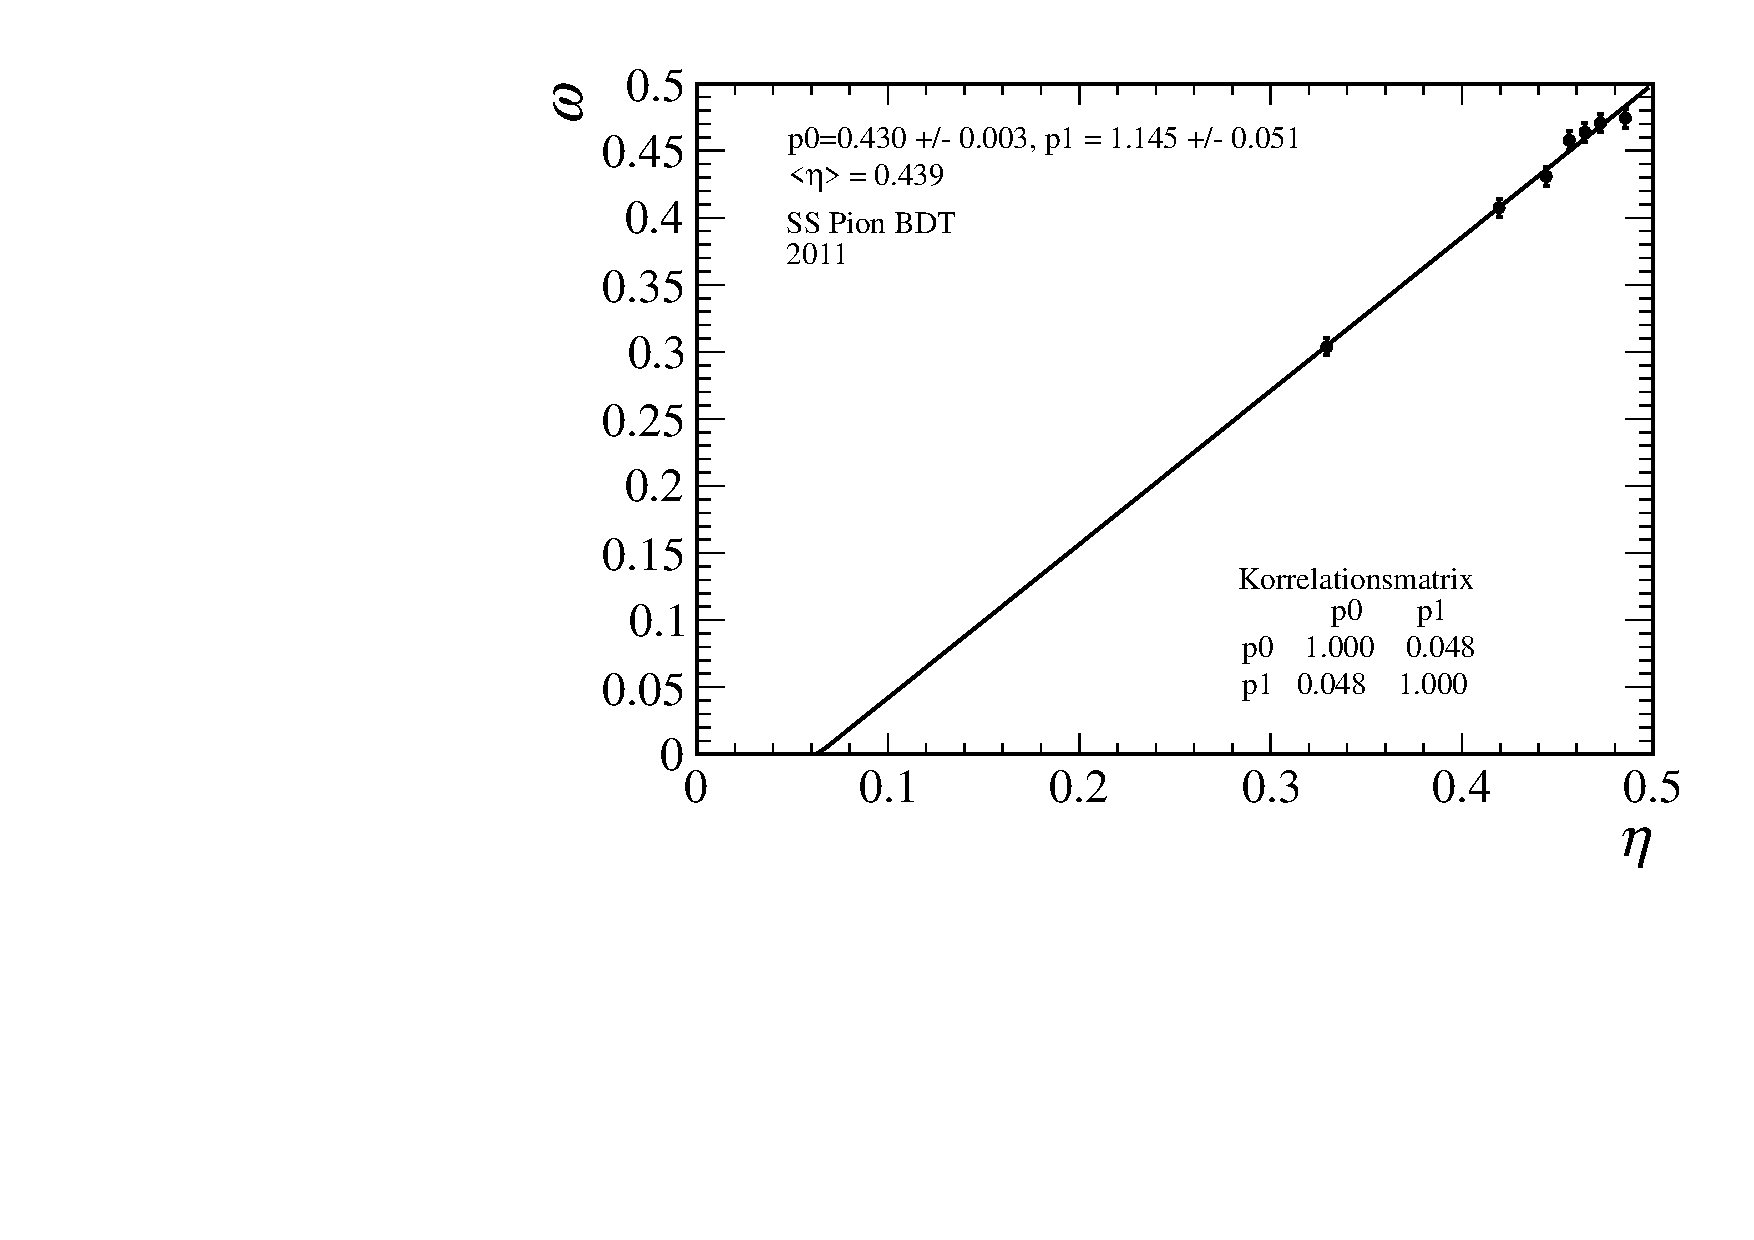
\includegraphics[width=0.49\textwidth]{fig/2011_SSPionBDT.pdf}
		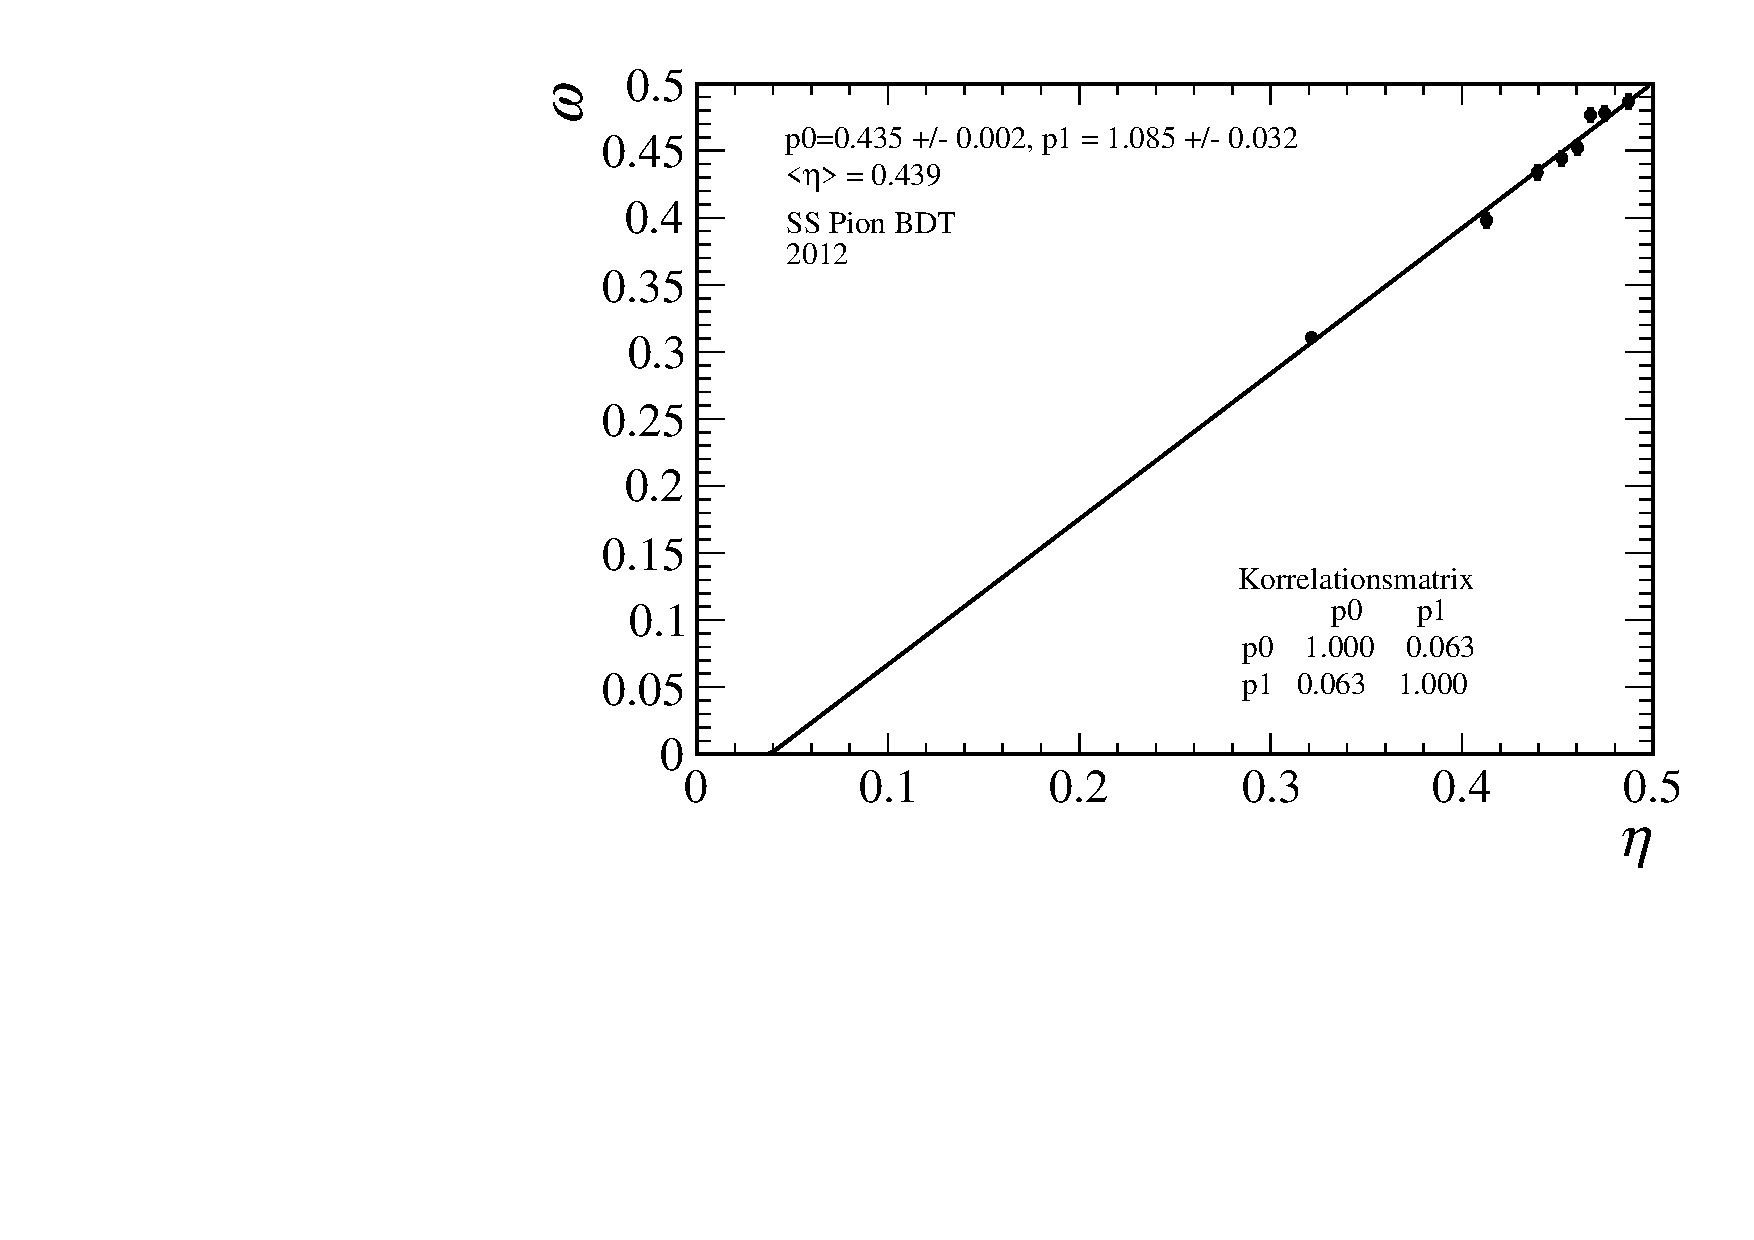
\includegraphics[width=0.49\textwidth]{fig/2012_SSPionBDT.pdf}
	\caption{Fit des linearen Zusammenhangs an die $(\eta,\omega)$-Paare für den SS Pion BDT Tagger auf Daten des Jahres \num{2011} (links) und \num{2012} (rechts) auf dem Kanal \BdToDpi.}
	\label{fig:fit_SSPionBDT} 
\end{figure}
\begin{table}[htbp]
	\centering
	\caption{Ergebnisse der Kalibrierung des SS Pion BDT Taggers für die Jahr \num{2011} und \num{2012} auf dem Kanal \BdToDpi.}
	\label{tab:result_SSPionBDT}
	\begin{tabular}{ccccc}
	\toprule
       Jahr & $\langle\eta\rangle$ & $p_0$ & $\left|p_0-\langle\eta\rangle\right|$ & $p_1$ \\ 
       \midrule 
	2011 & $0{.}439$ & $0{.}430\pm0{.}003$ & $0{.}009$ & $1{.}145\pm0{.}051$ \\
   	2012 & $0{.}439$ & $0{.}435\pm0{.}002$ & $0{.}004$ & $1{.}085\pm0{.}032$ \\ 
	\bottomrule
  \end{tabular}
\end{table}
Ebenso ist für das Jahr \num{2011} erkennbar, dass eine größere Anzahl Kategorien keinen Nutzen hätte. Auch sind die Parameter $p_0$ und $p_1$ beide um mehr als zwei Standardabweichungen von ihrem ideal kalibrierten Wert entfernt.
\begin{table}[htbp]
	\centering
	\caption{Performanz des SS Pion BDT Taggers für die Jahre \num{2011} und \num{2012} auf dem Kanal \BdToDpi.}
	\label{tab:performance_SSPionBDT}
	\begin{tabular}{ccccc}
	\toprule
      Jahr & $\varepsilon(\%)$ & $\omega$ & $D$ & $\varepsilon D^2(\%)$ \\ 
      \midrule
      2011 & $56{,}797\pm1{,}308$& $0{,}430\pm0{,}003$ & $0{,}140\pm0{,}006$ & $1{,}825\pm0{,}133$\\ 
      2012 & $58{,}147\pm0{,}141$& $0{,}435\pm0{,}002$ & $0{,}130\pm0{,}004$ & $1{,}656\pm0{,}070$\\ 
      \bottomrule
	\end{tabular}
\end{table}\\
Insgesamt lässt sich hier zunächst festhalten, dass der Tagger auf beiden Datensätzen sinnvolle Ergebnisse liefert. Dazu kann man hier die Taggingeffizienz $\varepsilon$ und die effektive Taggingeffizienz $\varepsilon D^2$ betrachten (Tabelle \ref{tab:performance_SSPionBDT}), die für beide Jahre ähnlich sind. Außerdem ist wie bei den zuvor untersuchten Taggern die effektive Taggingeffizienz für das Jahr \num{2012} etwas kleiner. Dies resultiert daraus, dass mit der höheren Rate der Datennahme auch die Selektion der Taggingkandidaten schwieriger und fehleranfäliger wird. Das spiegelt sich in höheren true-mistag-Wahrscheinlichkeiten $\omega$ wieder.\\
Im Vergleich zum schnittbasierten SS Pion Tagger stellt man weiterhin fest, dass der SS Pion BDT Tagger trotz seiner relativ schlechten true-mistag-Wahrscheinlichkeiten $\omega$ insgesamt um etwa \num{0{,}6} Prozentpunkte größere effektive Taggingeffizienzen $\epsilon D^2$ liefert. 

\subsection{Der SS Proton Tagger}

Für den SS Proton Tagger erhält man im Jahr \num{2011} eine Taggingeffizienz von $\varepsilon=\SI{33{,}775}{\%}$ und im Jahr \num{2012} von $\varepsilon=\SI{32{,}588}{\%}$. Die Ergebnisse der Kalibrierung sind in der Abbildung \ref{fig:fit_SSProton} und der Tabelle \ref{tab:result_SSProton} zu sehen. Man sieht auch hier wieder, dass trotz der großen Anzahl getaggter Ereignisse eine größere Anzahl an Kategorien nicht sinnvoll ist, da die mistag-Wahrscheinlichkeiten $\eta$ wieder sehr eng bei Werten größer $\num{0{,}4}$ verteilt sind. Für das Jahr \num{2012} weichen beide Parameter $p_0$ und $p_1$, wie beim SS Pion BDT Tagger, um zwei Standardabweichung von der idealen Kalibrierung ab, 
\begin{figure}[htbp]
	\centering
		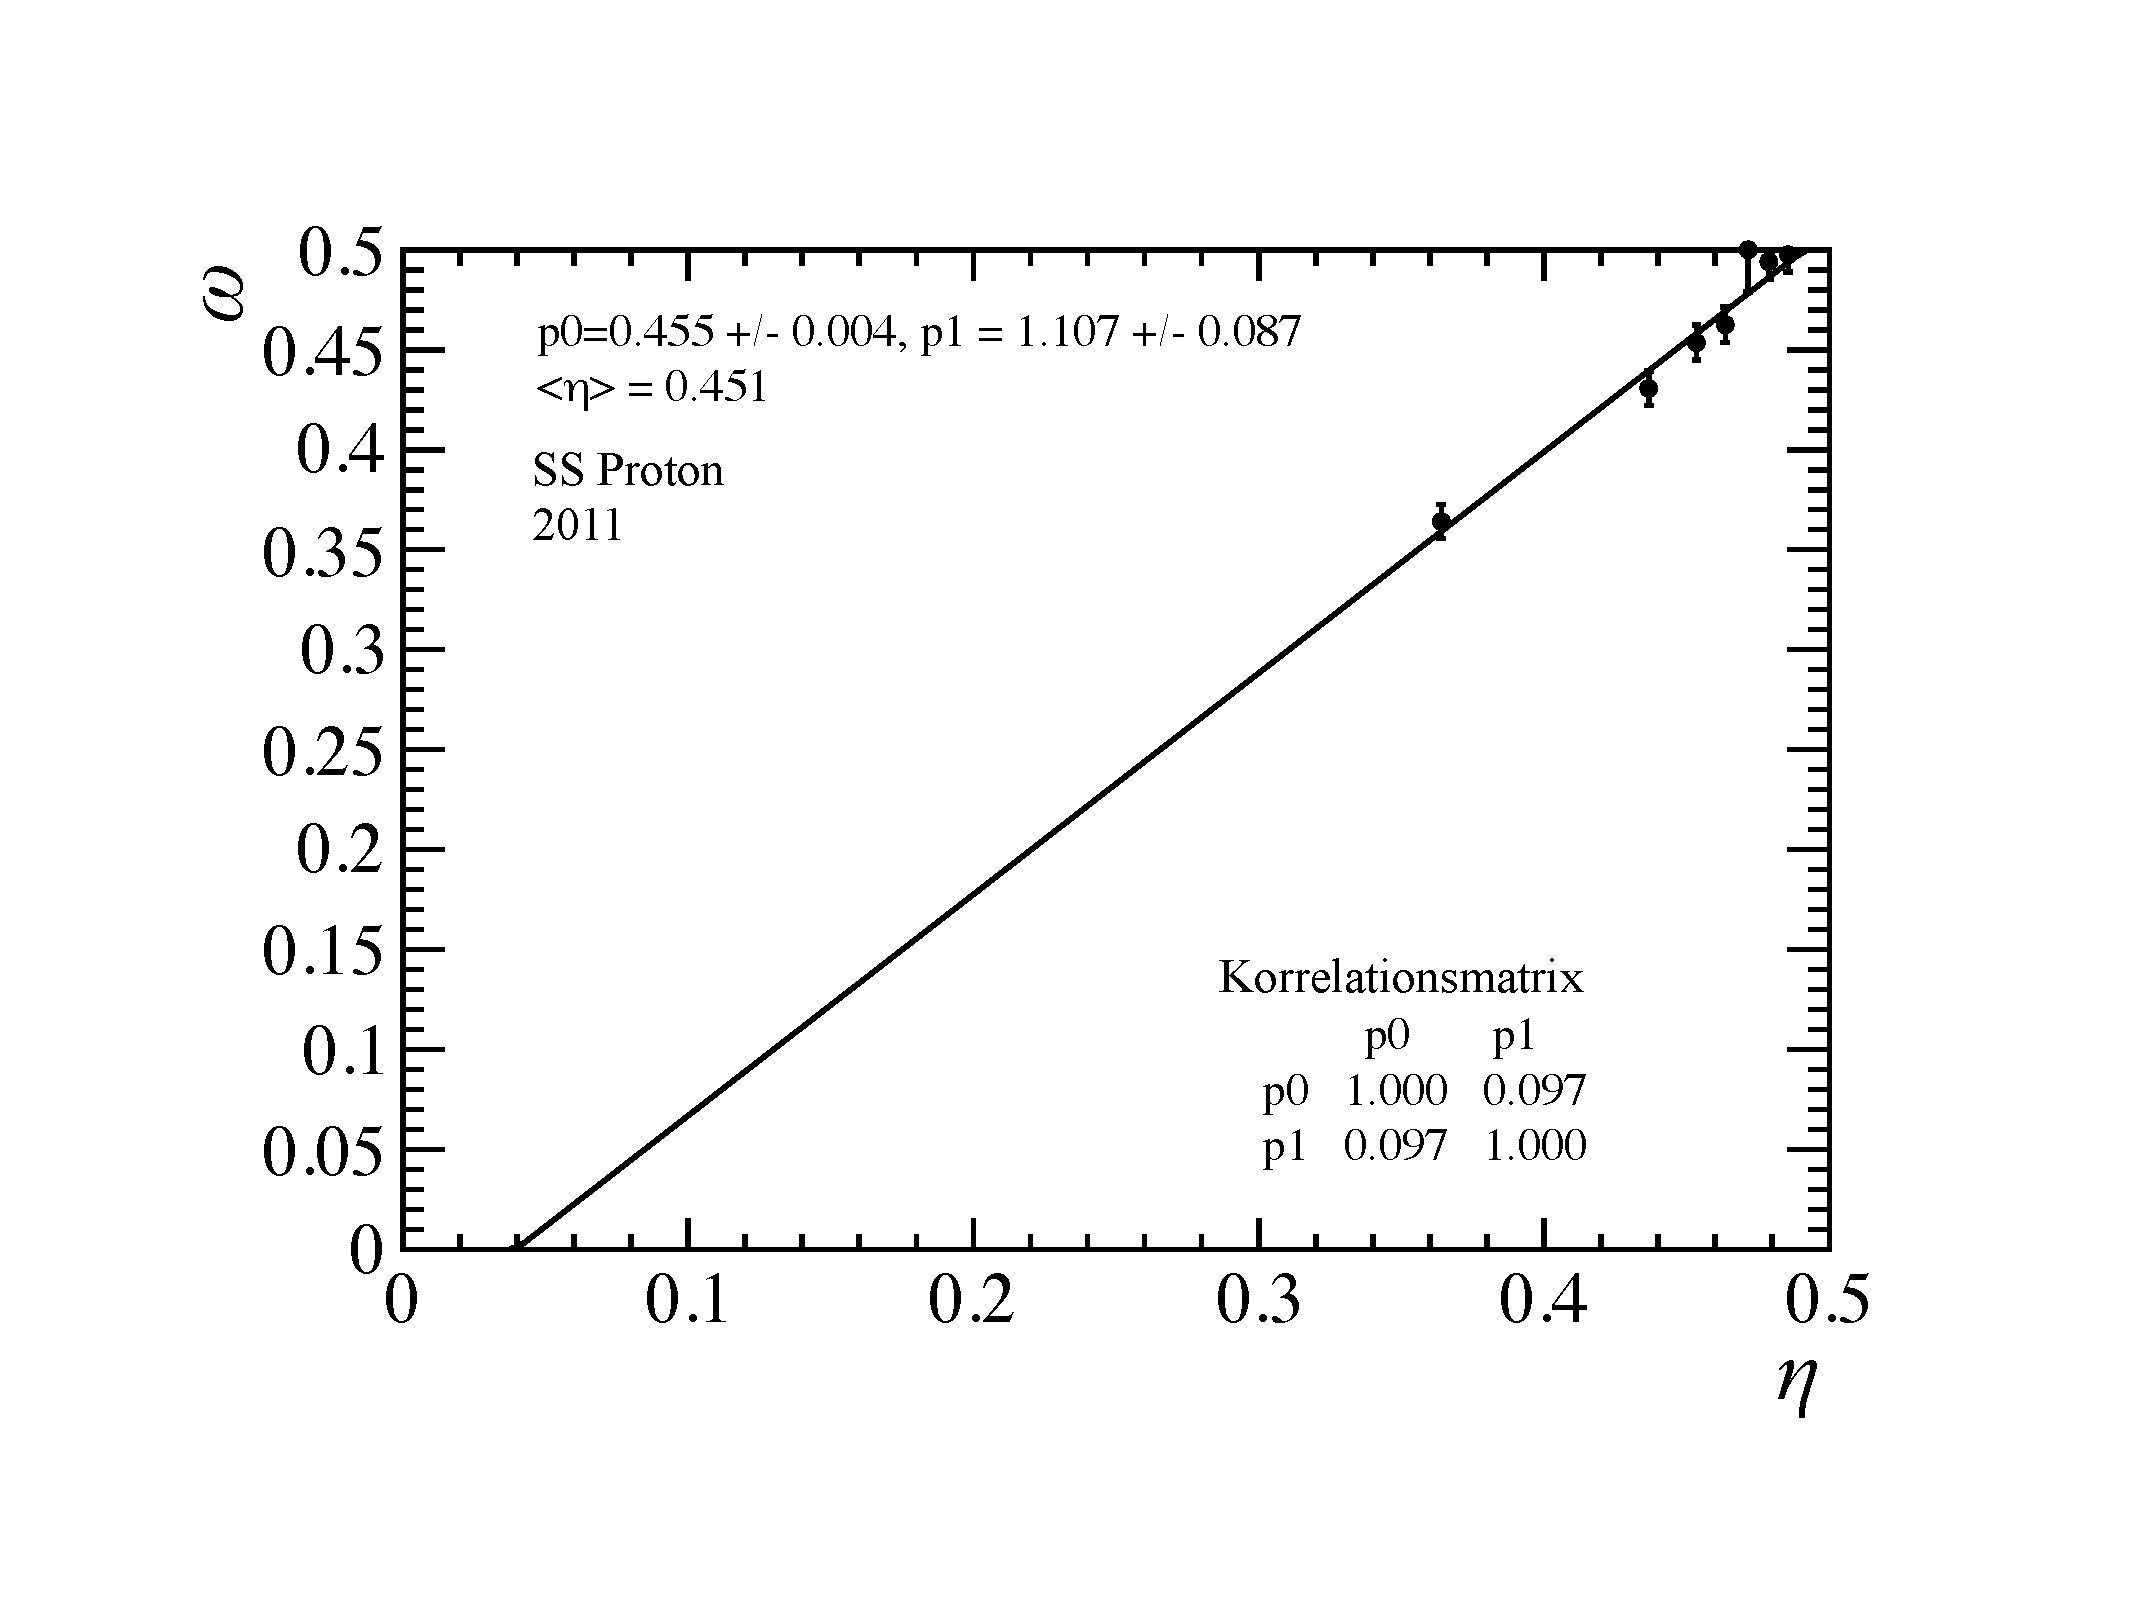
\includegraphics[width=0.49\textwidth]{fig/2011_SSProton.pdf}
		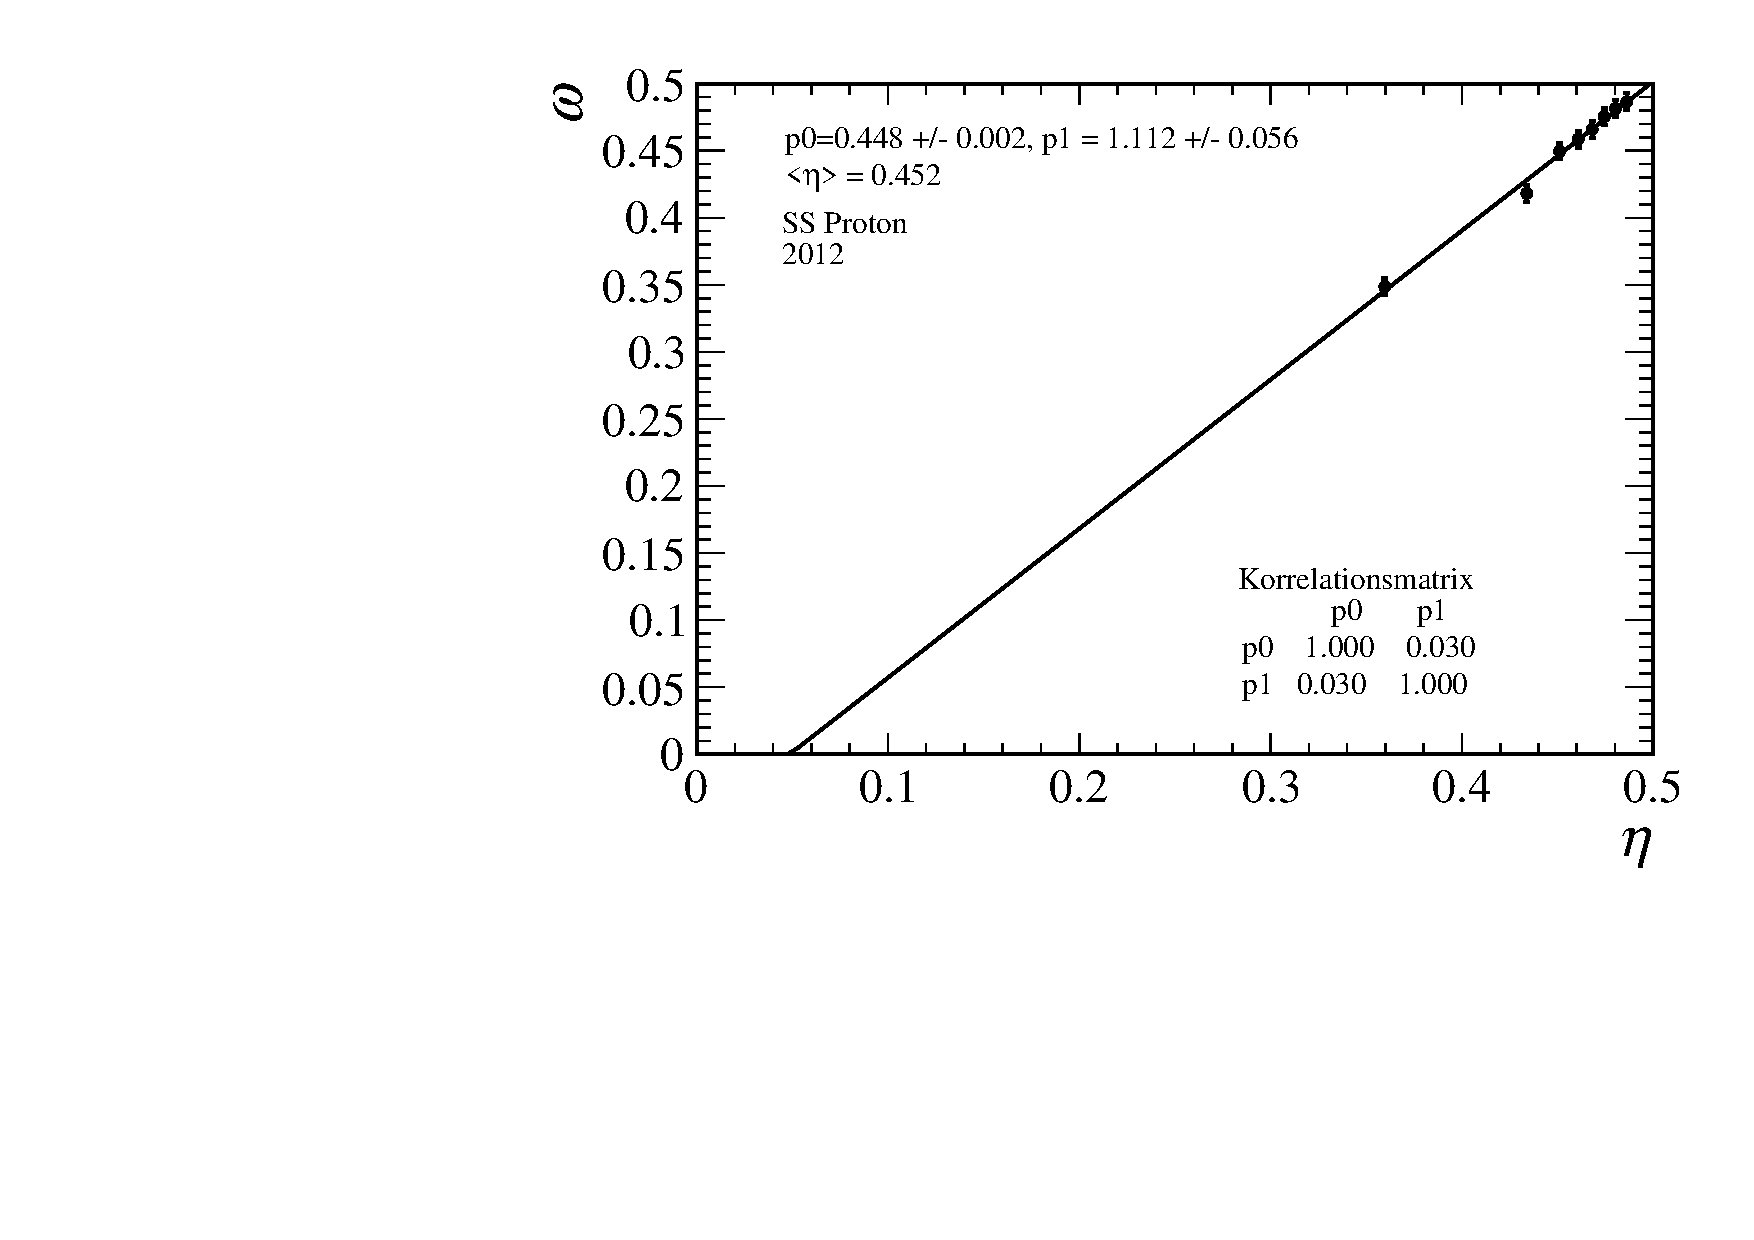
\includegraphics[width=0.49\textwidth]{fig/2012_SSProton.pdf}
	\caption{Fit des linearen Zusammenhangs an die $(\eta,\omega)$-Paare für den SS Proton Tagger auf Daten des Jahres \num{2011} (links) und \num{2012} (rechts) auf dem Kanal \BdToDpi.}
	\label{fig:fit_SSProton} 
\end{figure}
während die Abweichungen von der idealen Kalibrierung für das Jahr \num{2011}, aufgrund der größeren statistischen Unsicherheiten auf die Parameter $p_0$ und $p_1$, weniger signifikant sind.
\begin{table}[htbp]
	\centering
	\caption{Ergebnisse der Kalibrierung des SS Proton Taggers für die Jahre \num{2011} und \num{2012} auf dem Kanal \BdToDpi.}
	\label{tab:result_SSProton}
	\begin{tabular}{ccccc}
	\toprule
       Jahr & $\langle\eta\rangle$ & $p_0$ & $\left|p_0-\langle\eta\rangle\right|$ & $p_1$ \\ 
       \midrule
	2011 & $0{.}451$ & $0{.}455\pm0{.}004$ & $0{.}004$ & $1{.}107\pm0{.}087$ \\
   2012 & $0{.}452$ & $0{.}448\pm0{.}002$ & $0{.}004$ & $1{.}111\pm0{.}056$ \\ 
   \bottomrule
	\end{tabular}
\end{table}
\begin{table}[htbp]
	\centering
	\caption{Performanz des SS Proton Taggers für die Jahr \num{2011} und \num{2012} auf dem Kanal \BdToDpi.}
	\label{tab:performance_SSProton}
	\begin{tabular}{ccccc}
	\toprule
       Jahr & $\varepsilon(\%)$ & $\omega$ & $D$ & $\varepsilon D^2(\%)$ \\ 
       \midrule
   2011 & $33{,}775\pm0{,}785$& $0{,}455\pm0{,}003$ & $0{,}090\pm0{,}006$ & $0{,}528\pm0{,}062$\\ 
   2012 & $32{,}588\pm0{,}104$& $0{,}448\pm0{,}002$ & $0{,}104\pm0{,}004$ & $0{,}585\pm0{,}037$\\ 
   \bottomrule
	\end{tabular}
\end{table}
Gleich dem SS Pion BDT Tagger liefert der SS Proton Tagger auf beiden Datensätzen sinnvolle Ergebnisse. Die Taggingeffizienzen $\varepsilon$ und effektiven Taggingeffizienzen $\varepsilon D^2$ (Tabelle \ref{tab:performance_SSProton}) sind in der erwarteten Größenordnung, der mittlere true-mistag $\omega$ ist allerdings für das Jahr \num{2012} bei dem SS Proton Tagger etwas kleiner.

\section{Diskussion der Ergebnisse der Kalibrierung}

Bei der Betrachtung der Ergebnisse lässt sich zunächst die Kalibrierung selbst überprüfen. Um diese in Relation zu den Erwartungen zu setzen ist zu beachten, dass bei der verwendeten Version der Flavour-Tagging-Software alle etablierten Tagger bereits kalibriert sein sollten. Die Kalibrierungen wurden dabei jedoch auf neutralen Kanälen wie \BdToJPsiKst oder geladenen Kanälen wie \BuToJPsiKp vorgenommen.\\
Für die Tagger der Opposite Side ist die Kalibrierung unter diesen Bedingungen dabei in fast allen Fällen bestätigt; die Tagger können also in der aktuellen Version der Flavour-Tagging-Software als kalibriert angesehen werden. Einzig die Parameter des OS Kaon nnet weichen auf dem Datensatz aus dem Jahr \num{2012} beide so stark von den Erwartungen eines ideal kalibrierten Taggers ab, dass sich hier bei Analysen die diesen Tagger verwenden Probleme ergeben könnten. Bei den Taggern der Same Side ist zunächst etwas überraschend, dass der SS Pion Tagger auf dem hier untersuchten Kanal in beiden Jahren nicht kalibriert ist, da auch für diesen eine Präkalibration durchgeführt wurde. Allerdings sind bei den Taggern der Same Side auch durchaus größere Unterschiede zu erwarten, weil die Tagger stärker vom Signalzerfall und seiner Selektion beeinflusst sind. Da es sich bei den beiden auf \BdToDpi entwickelten Taggern, dem SS Pion BDT und dem SS Proton Tagger an dieser Stelle um die ersten unabhängigen Gegenproben handelt, liegt der Fokus hier weniger auf einer idealen Kalibration. Bei beiden Taggern liefert die Kalibrierung sinnvolle Ergebnisse für die Taggingeffizienz $\varepsilon$ und die effektive Taggingeffizienz $\varepsilon D^2$. Außerdem lässt sich an dieser Stelle ein erster Vergleich zwischen dem SS Pion und dem SS Pion BDT Tagger ziehen. Hier sieht man, dass der SS Pion BDT Tagger in der effektiven Taggingeffizienz $\varepsilon D^2$ einen Zuwachs bringt. Einzig herausfordernd wären hier mögliche größere Korrelationen des SS Pion BDT Taggers gegenüber dem SS Pion Tagger mit anderen Taggern.\\
Weiterhin lassen sich die Tagger bezüglich ihrer effektiven Taggingeffizienzen $\varepsilon D^2$ für die Jahre \num{2011} und \num{2012} vergleichen. Obwohl bei allen Taggern die Taggingeffizienz $\varepsilon$ etwa gleich bleibt, ist hier zu erkennen, dass bis auf den SS Proton hier bei alle Taggern  $\varepsilon D^2$ für die Daten des Jahres \num{2012} im Vergleich zu den Daten des Jahres \num{2011} sinkt (Tabelle \ref{tab:diskussion}). Eine mögliche Ursache ist die höhere instantane Luminosität im Jahr \num{2012}. Durch die größere Anzahl an Protonenkollisionen bei einer einzelnen Strahlkollision ist es für die Taggingalgorithmen schwieriger die Taggingteilchen zu finden. Somit verschlechtern sich die Einschätzungen der Tagger, was sich direkt im true-mistag $\omega$ niederschlägt. Auch dieser Effekt, der schlechter werdenden true-mistag-Wahrscheinlichkeiten ist in den Ergebnissen zu erkennen. Einzig die Abweichung im Verhalten des SS Proton Taggers muss noch weiter untersucht werden.
\begin{table}[htbp]
	\centering
	\caption{Zusammenfassung der Ergebnisse der Taggingeffizienzen $\varepsilon$ und der effektiven Taggingeffizienzen $\varepsilon D^2$ der Kalibrierungen.}
	\label{tab:diskussion}
	\begin{tabular}{ccccc}
	\toprule
       		& \multicolumn{2}{c}{$\varepsilon(\%)$} & \multicolumn{2}{c}{$\varepsilon D^2(\%)$}\\
		& \num{2011} & \num{2012} & \num{2011} & \num{2012} \\ 
		\midrule
   OS Std. Komb. & $37{,}449\pm0{,}814$& $38{,}366\pm0{,}112$ & $3{,}777\pm0{,}183$ & $3{,}597\pm0{,}091$\\ 
   OS Charm & $3{,}304\pm0{,}102$& $3{,}264\pm0{,}032$ & $0{,}512\pm0{,}049$ & $0{,}395\pm0{,}041$\\ 
   OS Kaon nnet & $45{,}044\pm1{,}041$& $46{,}459\pm0{,}125$ & $1{,}621\pm0{,}122$ & $1{,}588\pm0{,}061$\\ 
   SS Pion & $14{,}847\pm0{,}380$& $15{,}146\pm0{,}070$ & $1{,}104\pm0{,}074$ & $1{,}071\pm0{,}049$\\ 
   SS Pion BDT & $56{,}797\pm1{,}308$& $58{,}147\pm0{,}141$ & $1{,}825\pm0{,}133$ & $1{,}656\pm0{,}070$\\ 
   SS Proton & $33{,}775\pm0{,}785$& $32{,}588\pm0{,}104$ & $0{,}528\pm0{,}062$ & $0{,}585\pm0{,}037$\\ 
   \bottomrule
   \end{tabular}
\end{table}

\section{Korrelation zwischen Taggern der Same Side}

Der neue SS Proton Tagger untersucht, wie der etablierte SS Pion oder auch auch der neue SS Pion BDT Tagger, den Hadronisierungsprozess eines \dquark-Quarks auf der Same Side. Aufgrund dieser Ähnlichkeit soll zwischen diesen Taggern, vor allem zwischen dem SS Proton Tagger und den beiden Pionen Taggern die Möglichkeit einer bestehenden Korrelation untersucht werden. Eine mögliche Korrelation bestünde, wenn im Hadronisierungsprozess des Pions auf der Same Side direkt ein Proton entsteht. Dieses würde für den SS Proton Tagger zur gleichen Entscheidung führen wie das Pion für den SS Pion Tagger. Um dabei zunächst einen Einblick zu erhalten, wie stark diese Korrelation sein kann, wird das Verhältnis an Ereignissen $R_\text{Überlapp}$ berechnet, bei der beide Tagger für dieselben Ereignisse eine Entscheidung treffen, relativ zur Gesamtzahl der von beiden Taggern getroffenen Entscheidungen:
\begin{equation}
R_\text{Überlapp}=\frac{N_{\pi+\proton}}{N_{\pi,exkl}+N_{\proton,exkl}+N_{\pi+\proton}}.
\end{equation}
Dabei bezeichnet $N_{\pi+\proton}$ die Anzahl Ereignisse, in der sowohl der entsprechende Pion Tagger eine Entscheidung getroffen hat, als auch der SS Proton Tagger und $N_{\pi,exkl}$ und $N_{\proton,exkl}$ sind die Anzahl Ereignisse, in denen der entsprechende Pionen Tagger beziehungsweise der SS Proton Tagger jeweils exklusiv eine Entscheidung getroffen haben. Für den Vergleich zwischen dem SS Pion Tagger und dem SS Proton Tagger erhält man so $R_\text{Überlapp}=\SI{11{,}89}{\%}$ und für den Vergleich zwischen SS Pion BDT Tagger und SS Proton Tagger ein Verhältnis von $R_\text{Überlapp}=\SI{31{,}18}{\%}$. Eine mögliche Korrelation wäre also zwischen dem SS Pion BDT Tagger und dem SS Proton Tagger schwerwiegender als zwischen dem SS Proton Tagger und dem SS Pion Tagger.\\
Im nächsten Schritt wird betrachtet, wie oft beide Tagger jeweils gleiche  oder unterschiedliche Entscheidungen treffen. Die Ergebnisse dazu sind in Tabelle \ref{tab:overlap} dargestellt. Man erkennt, dass auch hier die Anzeichen aufgrund der etwas größeren Diskrepanz zwischen gleichen und unterschiedlichen Entscheidungen für eine mögliche Korrelation zwischen dem SS Pion BDT und dem SS Proton Tagger stärker sind, als bei dem SS Pion und dem SS Proton Tagger. Zum Vergleich ist weiterhin der Überlapp $R_\text{Überlapp}$ zwischen dem SS Pion und dem SS Pion BDT Tagger gezeigt. Bei diesen beiden Taggern erwartet man eine nahezu vollständige Korrelation, da sie die gleichen Teilchen für ihre Tagentscheidung nutzen.
\begin{table}[htbp]
	\centering
	\small
	\caption{Verhältnis gleicher und unterschiedlicher Entscheidungen zur Einschätzung der Korrelation. Die absoluten Anzahlen werden dabei durch $N$ bezeichnet, die relativen Verhältnisse zum gesamten Überlapp der beiden Tagger jeweils mit $R$. Weiterhin bezeichnet $d_i=d_j$ die Fälle mit gleichen Tags und $d_i\neq d_j$ die Fälle mit ungleichen Tags.}
	\label{tab:overlap}
	\begin{tabular}{ccccccc}
	\toprule
         			& \multicolumn{2}{c}{SS$_\pi$ \& SS$_\proton$} & \multicolumn{2}{c}{SS$_{\pi\text{BDT}}$ \& SS$_\proton$} & \multicolumn{2}{c}{SS$_\pi$ \& SS$_{\pi\text{BDT}}$} \\  
        				& $N$ & $R \si{ [\percent]}$ & $N$ & $R \si{ [\percent]}$ & $N$ & $R \si{ [\percent]}$ \\ 
				\midrule
       $d_i=d_j$	& $9562\pm98$ & $51{,}2\pm0{,}6$ & $42360\pm206$ & $53{,}1\pm0{,}3$ &  $46338\pm215$  & $90{,}6\pm0{,}6$ \\ 
        $d_i\neq d_j$  & $9096\pm95$ & $48{,}8\pm0{,}6$ & $37418\pm193$ & $46{,}9\pm0{,}3$ & $4799\pm69$  & $9{,}4\pm0{,}1$ \\ 
        \bottomrule
	\end{tabular}
\end{table}\\
Man erkennt hier, dass Anzeichen für eine leichte Korrelation vor allem zwischen SS Pion BDT und SS Proton Tagger bestehen, da das Verhältnis $R$ signifikant von \SI{50}{\%} abweicht.\\
Im Folgenden werden nun Korrelationen zwischen den Verteilungen der mistag-Wahrscheinlichkeiten $\eta$ gegeneinander untersucht. Zum Vergleich ist hier  die Kombination aus SS Pion und SS Pion BDT Tagger für zwei stark korrelierte Tagger und die Kombination aus SS Pion Tagger und der OS Kombination für zwei unkorrelierte Tagger gezeigt. In den Abbildungen \ref{fig:SSp_SSpi}, \ref{fig:SSp_SSpiBDT}, \ref{fig:SSpi_SSpiBDT} und \ref{fig:SSpi_OS} sind die Vergleiche der 2D-mistag-Verteilungen dargestellt. Bei einer starken Korrelation erwartet man, wie für den Vergleich des SS Pion und des SS Pion BDT Taggers zu sehen, diagonale Strukturen. Für die Kombinationen des SS Proton Taggers mit den beiden Pionen Taggern ist aber vor allem eine gleichmäßige Verteilung der mistag-Wahrscheinlichkeiten um eine Häufung in der oberen rechten Eckte der Plots zu erkennen. Die waagerechten und senkrechten Strukturen, die teilweise zu sehen sind, deuten nicht auf eine Korrelation, sondern auf spezielle Ausprägungen der einfachen mistag-Verteilungen hin.
\begin{figure}[htbp]
	\centering
		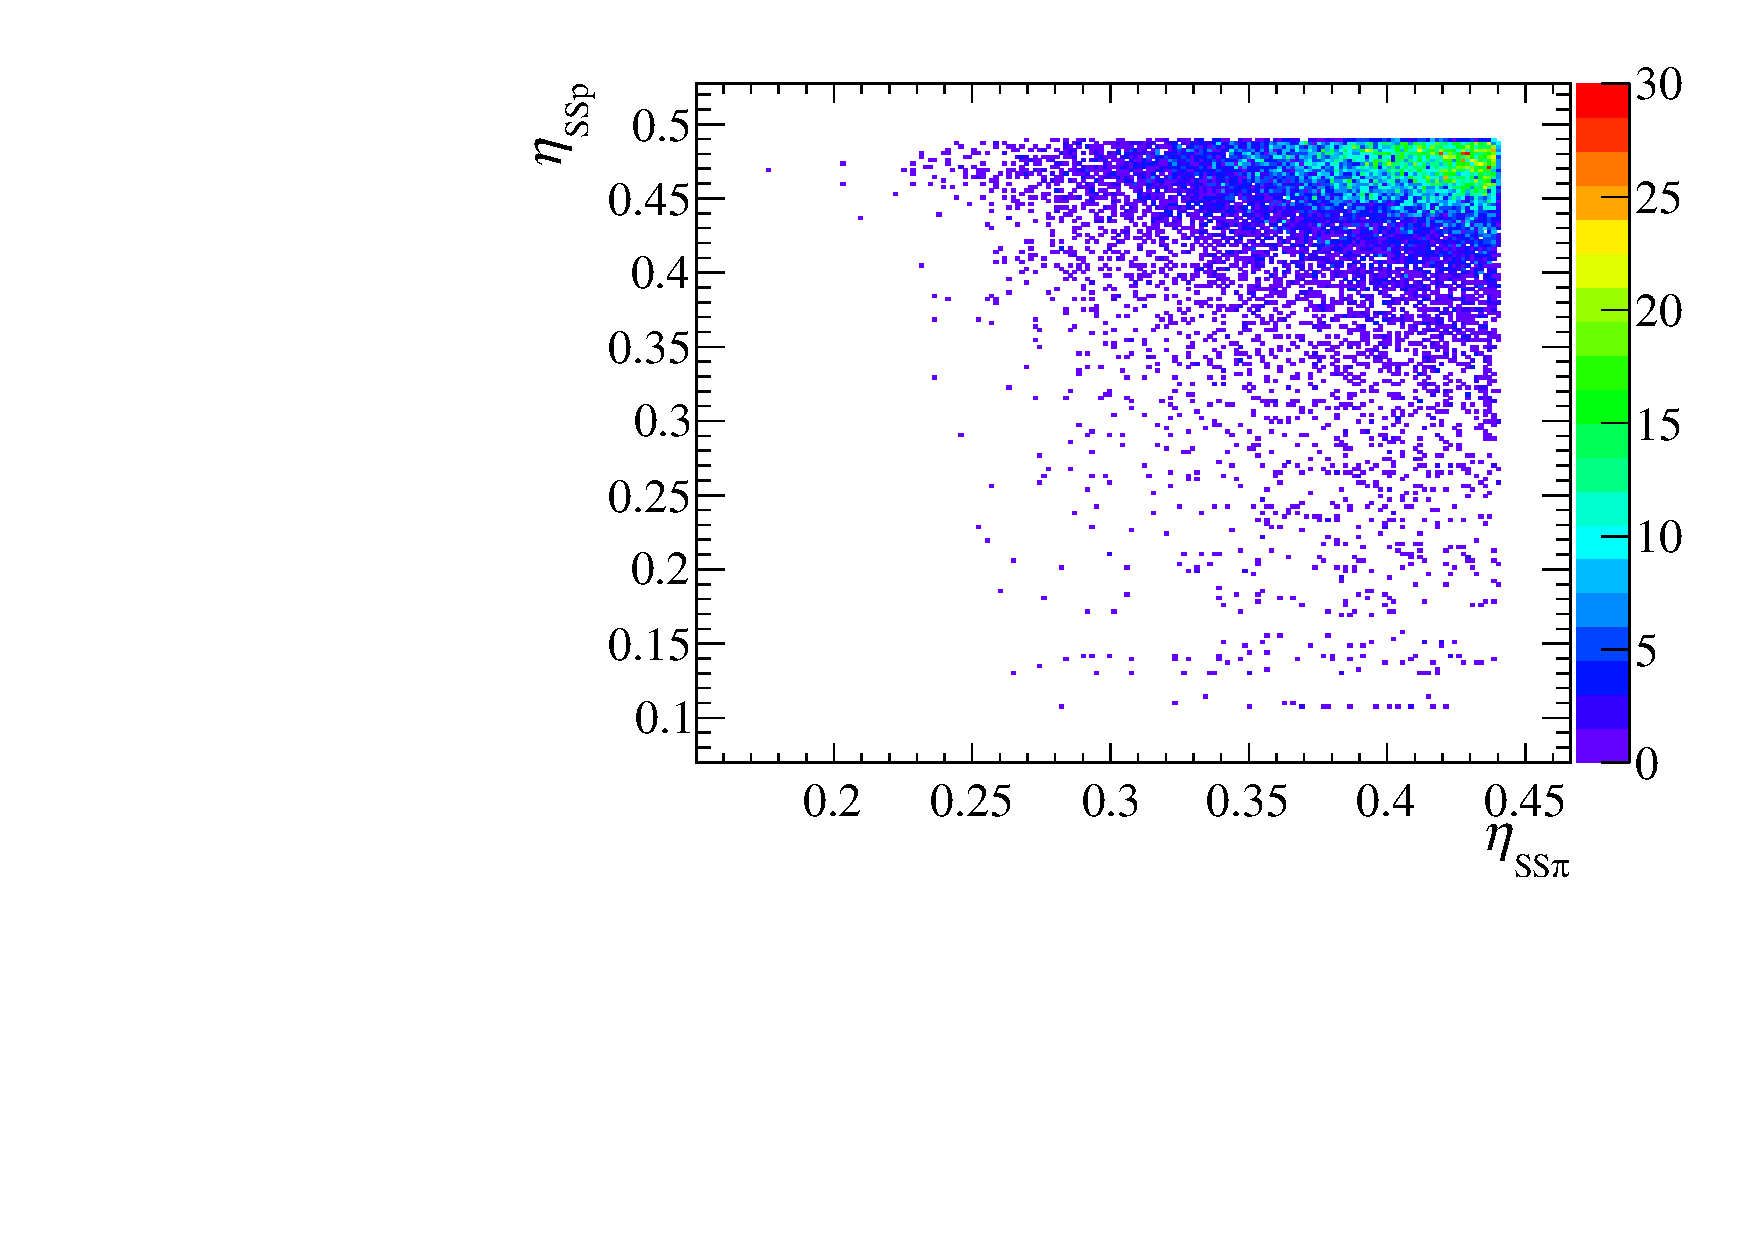
\includegraphics[width=0.75\textwidth]{fig/SSp_SSpi.pdf}
	\caption{Zweidimensionale Darstellung der $\eta$-Verteilungen des SS Proton und des SS Pion Taggers. Es sind keine diagonalen Strukturen, die auf eine Korrelation schließen ließen, erkennbar.}
	\label{fig:SSp_SSpi} 
\end{figure}
\begin{figure}[htbp]
	\centering
		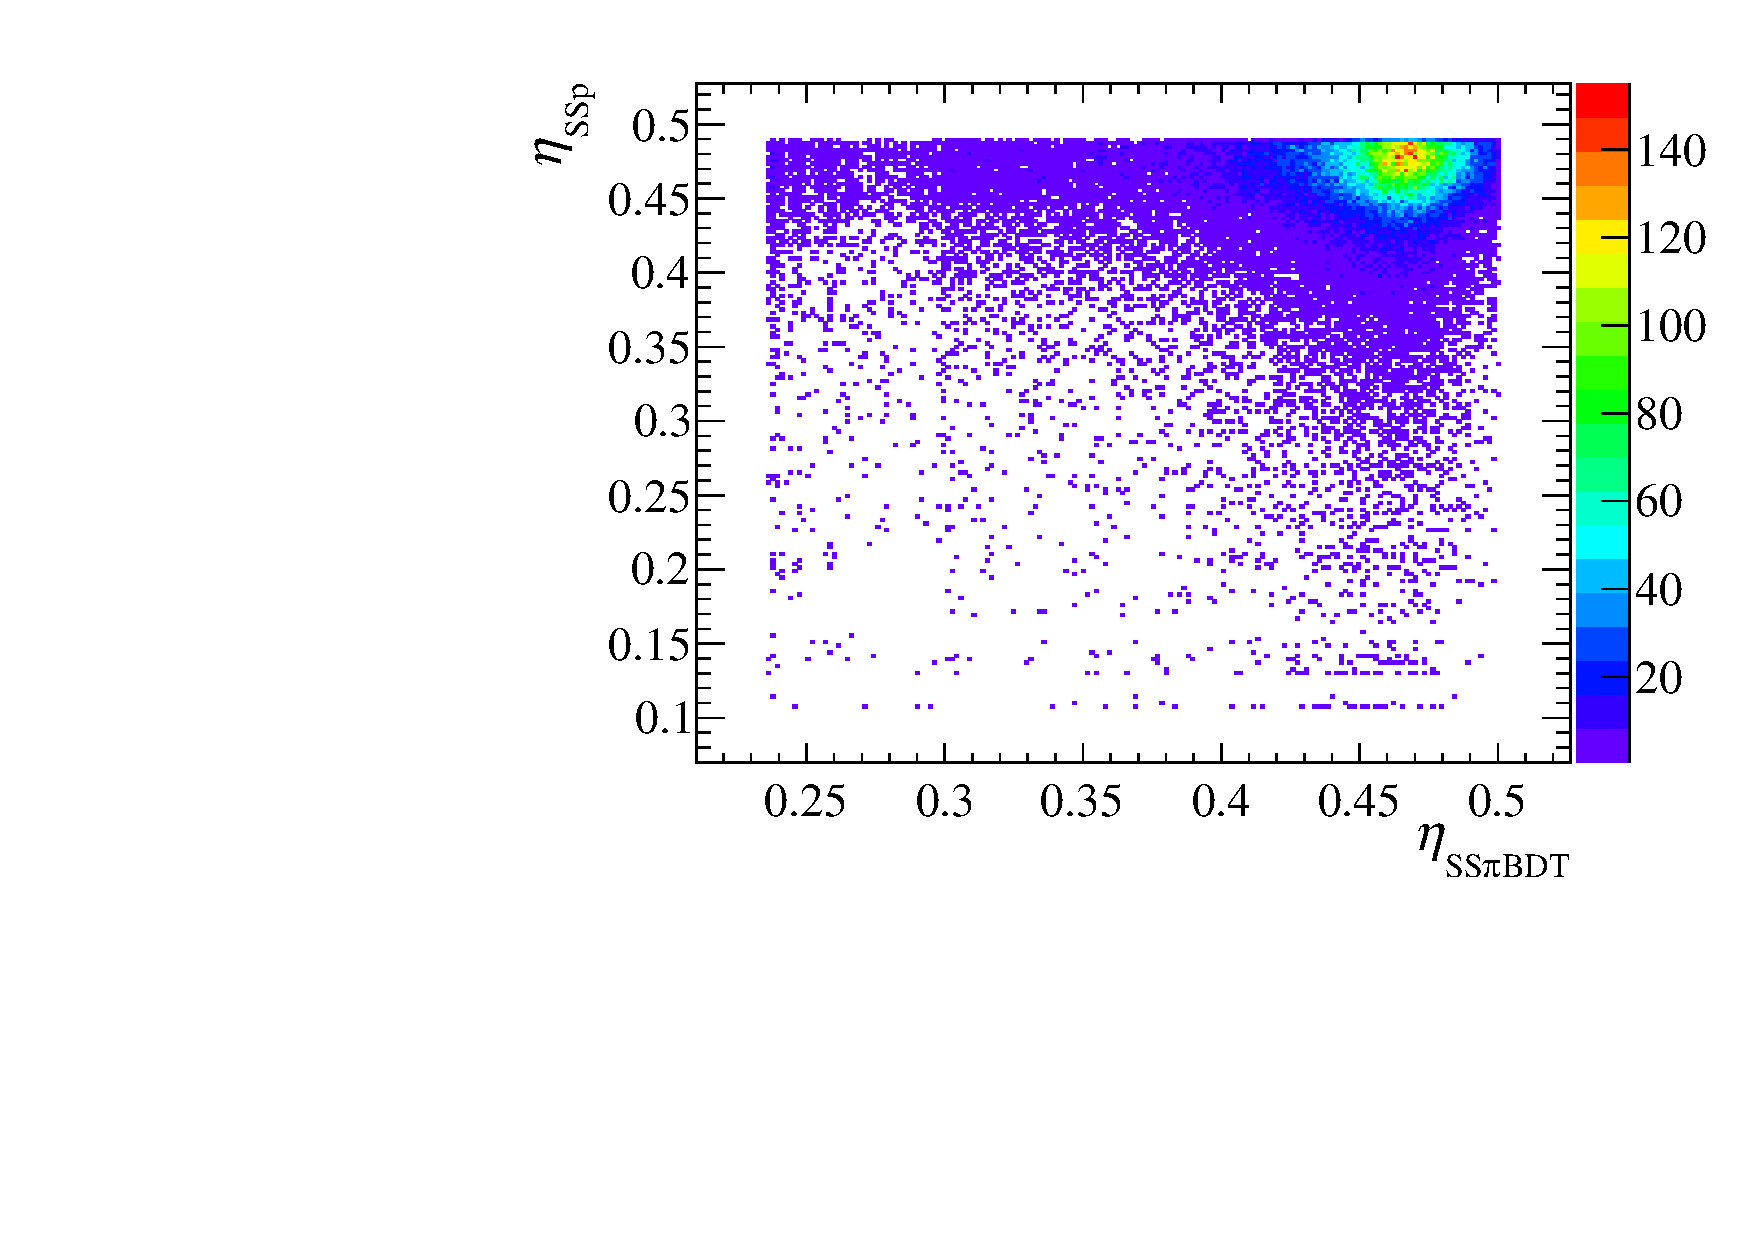
\includegraphics[width=0.75\textwidth]{fig/SSp_SSpiBDT.pdf}
	\caption{Zweidimensionale Darstellung der $\eta$-Verteilungen des SS Proton und des SS Pion BDT Taggers. Es sind keine diagonalen Strukturen, die auf eine Korrelation schließen ließen, erkennbar.}
	\label{fig:SSp_SSpiBDT} 
\end{figure}
\begin{figure}[htbp]
	\centering
		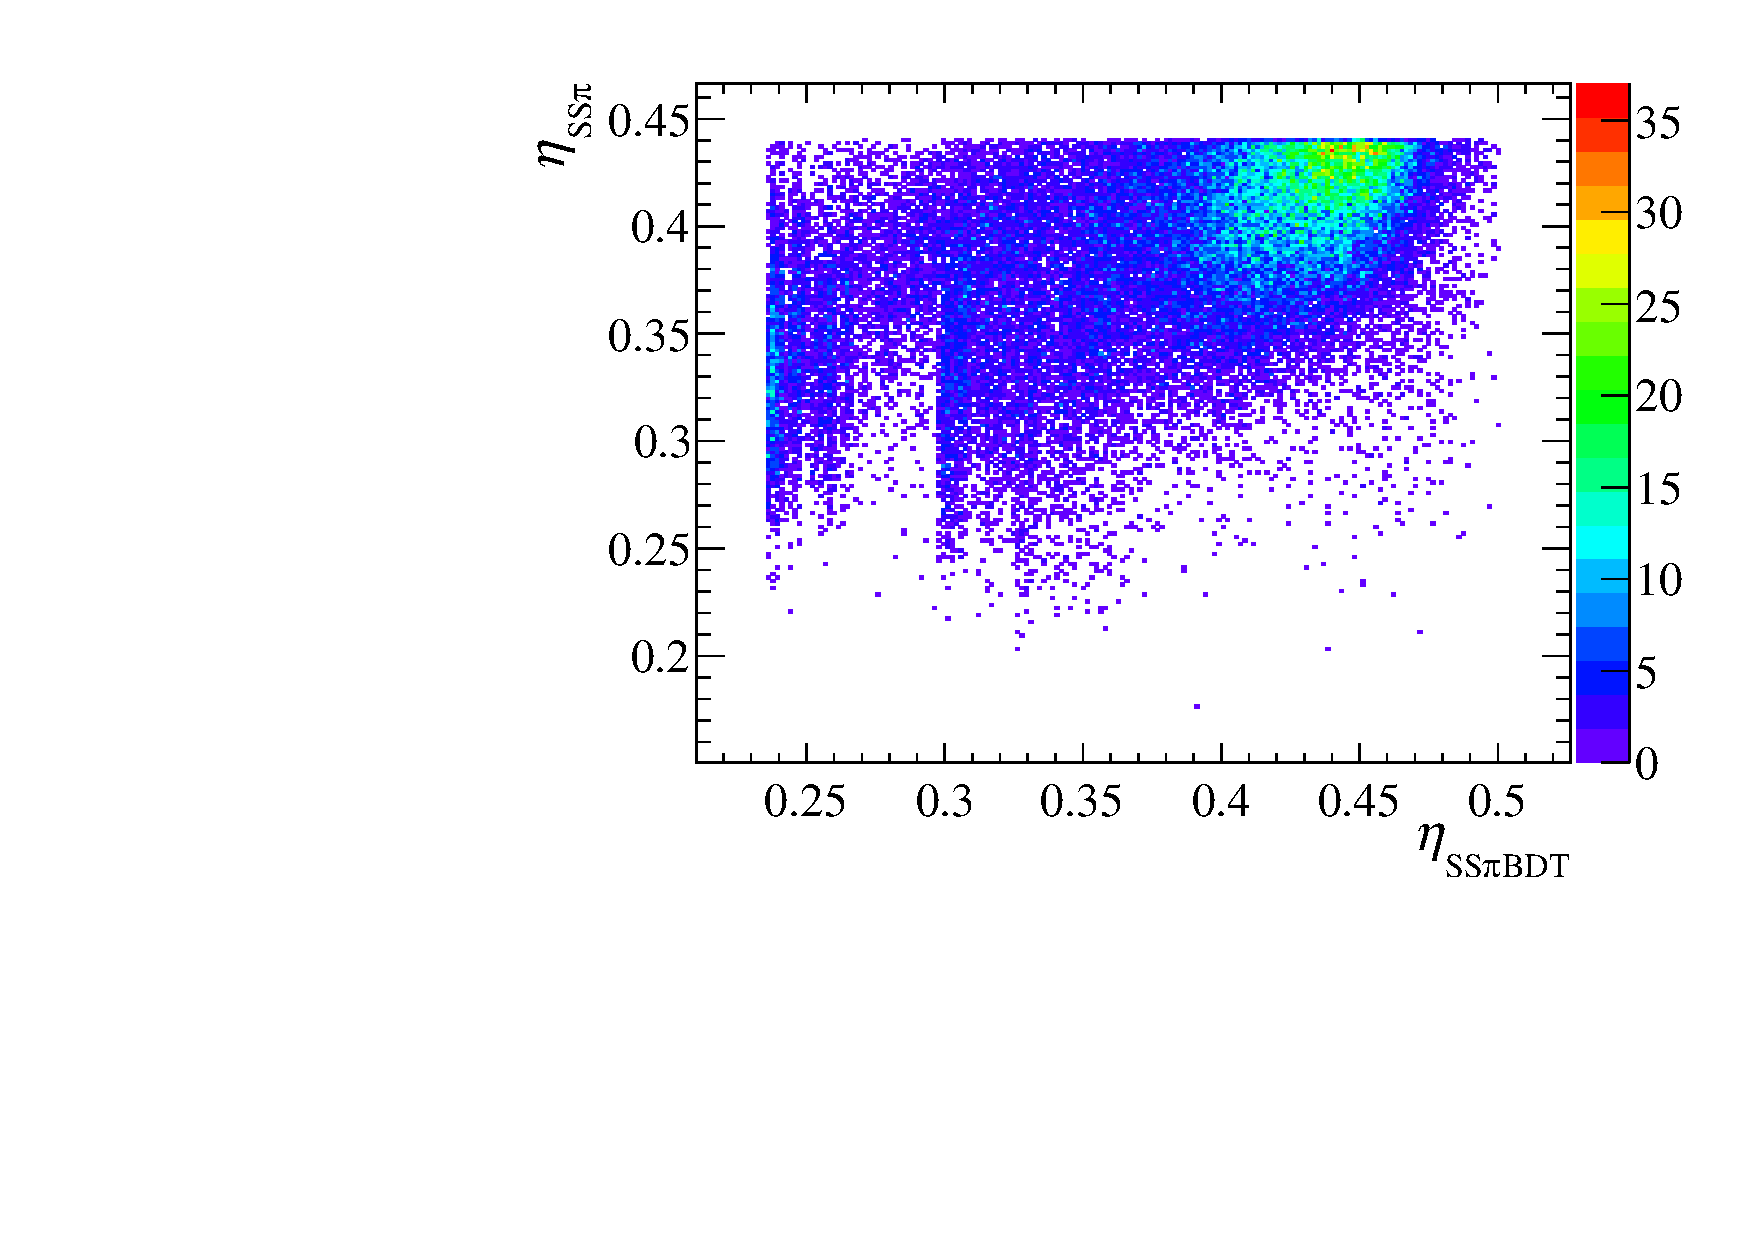
\includegraphics[width=0.75\textwidth]{fig/SSpi_SSpiBDT.pdf}
	\caption{Zweidimensionale Darstellung der $\eta$-Verteilungen des SS Pion BDT und des SS Pion Taggers. Es sind diagonalen Strukturen, die auf eine Korrelation schließen lassen, erkennbar.}
	\label{fig:SSpi_SSpiBDT} 
\end{figure}
\begin{figure}[htbp]
	\centering
		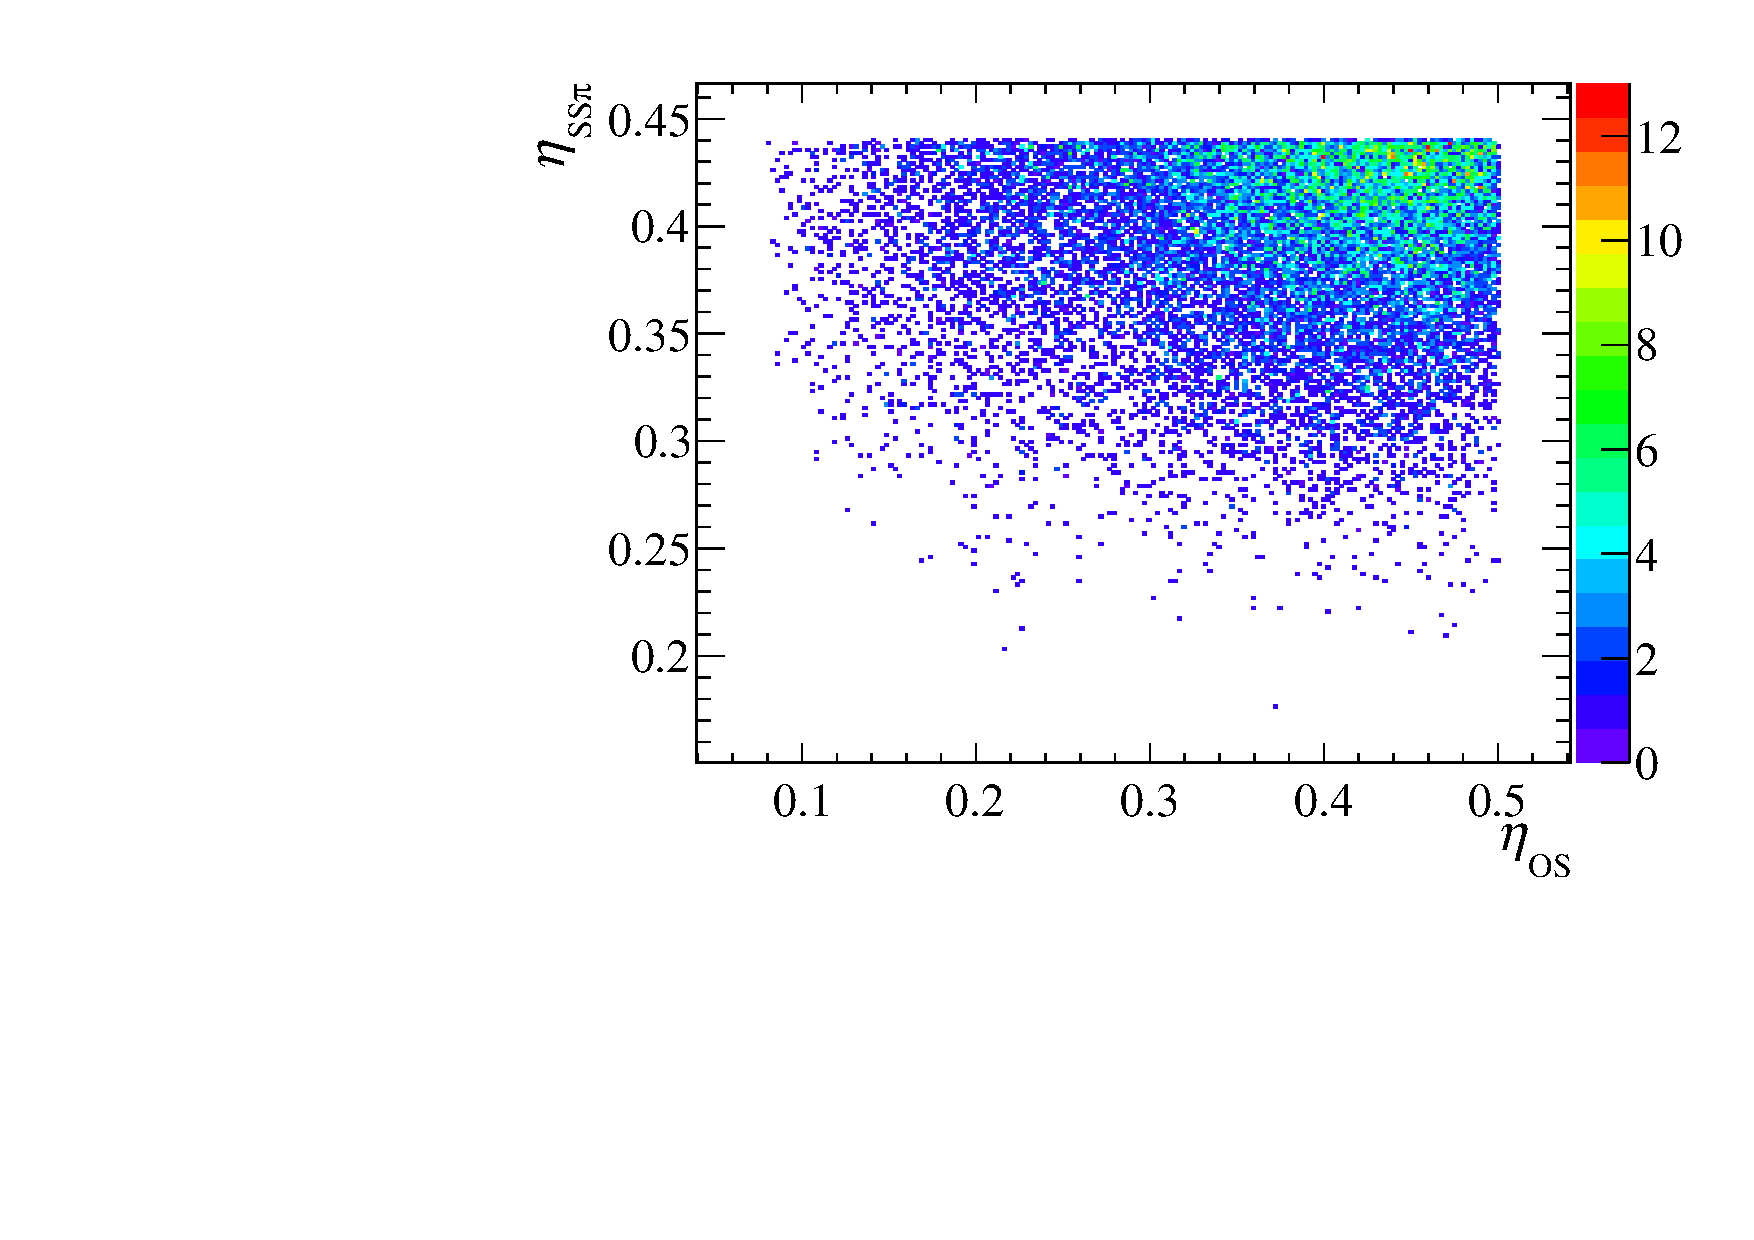
\includegraphics[width=0.75\textwidth]{fig/SSpi_OS.pdf}
	\caption{Zweidimensionale Darstellung der $\eta$-Verteilungen der OS Kombination und des SS Pion Taggers. Es sind keine diagonalen Strukturen, die auf eine Korrelation schließen ließen, erkennbar.}
	\label{fig:SSpi_OS} 
\end{figure}
Weiter lässt sich für die Verteilungen der Korrelationskoeffizient nach Pearson \cite{Blobel}
\begin{equation}
\rho(\eta_i,\eta_j)=\frac{\text{Cov}(\eta_i,\eta_j)}{\sigma(\eta_i)\sigma(\eta_j)}\label{eq:rho_koeff}
\end{equation}
berechnen. Die Ergebnisse mit einem \SI{95}{\%} Konfidenzintervall $P_{\SI{95}{\%}}$ sind in Tabelle \ref{tab:pearson_coeff} dargestellt.
\begin{table}[htbp]
	\centering
	\caption{Korrelationskoeffizienten nach Gleichung \eqref{eq:rho_koeff} für die drei untersuchten Tagger Kombinationen. Außerdem ist für jeden Wert das \SI{95}{\%} Konfidenzintervall $P_{\SI{95}{\%}}$ angegeben.}
	\label{tab:pearson_coeff}
	\begin{tabular}{ccccc}
	\toprule
         			& SS$_\pi$ \& SS$_\proton$ & SS$_{\pi\text{BDT}}$ \& SS$_\proton$ & SS$_\pi$ \& SS$_{\pi\text{BDT}}$ & OS \& SS$_\pi$ \\ 
			\midrule
       $\rho$		& \num{0{,}057} & \num{0{,}122} & \num{0{,}522} & \num{0{,}042} \\ 
       $P_{\SI{95}{\%}}$  & $[0{,}042;0{,}074]$ & $[0{,}113;0{,}132]$ & $[0{,}515;0{,}529]$ & $[0{,}027;0{,}058]$  \\ 
       \bottomrule
	\end{tabular}
\end{table}
Man erkennt hier die deutliche Korrelation zwischen den mistag-Verteilungen der beiden Pionen Tagger. Außerdem ist auch hier die mistag-Verteilung des SS Proton stärker mit der des SS Pion BDT korreliert, als mit der mistag-Verteilung des SS Pion Taggers. Vergleicht man die Korrelation des SS Proton Taggers mit dem SS Pion Tagger mit der Korrelation zwischen der OS Kombination und dem SS Pion Tagger, so können diese in den Grenzen des Konfidenzintervalls, als nahezu unkorreliert angenommen werden.

\section[head={Messung von $\dmd$},tocentry={Messung von $\dmd$}]{Messung von $\mathbf{\dmd}$}

Bei der Kalibrierung der verschiedenen Tagger wird bei der Messung der Mischungsasymmetrie auch immer die Frequenz \dmd der Oszillation der neutralen \Bz-Mesonen gemessen. Da die Frequenz und die Amplitude dieser Asymmetrie nicht miteinander korreliert sind, hat der Parameter \dmd keinen Einfluss auf die bisherigen Kalibrierung der Tagger und lässt sich als Mischungsfrequenz bestimmen. Da der Parameter \dmd zwischen den einzelnen Kategorien der mistag-Wahrscheinlichkeit geteilt wird, steht in einem einzelnen Fit die gesamte Statistik eines Taggers zur Verfügung.\\
Da es auf dem Kanal \BdToDpi zukünftig noch eine offizielle Messung von \dmd geben kann und diese nicht beeinflusst werden soll, wird die hier durchgeführte Messung durch Addition eines unbekannten Offset \enquote{blind} gemacht. Es ist an dieser Stelle also nicht möglich, einen gemessenen Zentralwert zu präsentieren. Allerdings lässt sich durch Betrachtung der in den Abbildungen \ref{fig:dmd_mass}, \ref{fig:dmd_time} und \ref{fig:dmd_asymmetry} dargestellten Massen- und Zeitfits und Mischungsasymmetrie sehen, dass der durchgeführte Fit funktioniert und die weiteren erhaltenen Parameterwerte sinnvolle Ergebnisse liefern sollten. 
\begin{figure}[htbp]
	\centering
		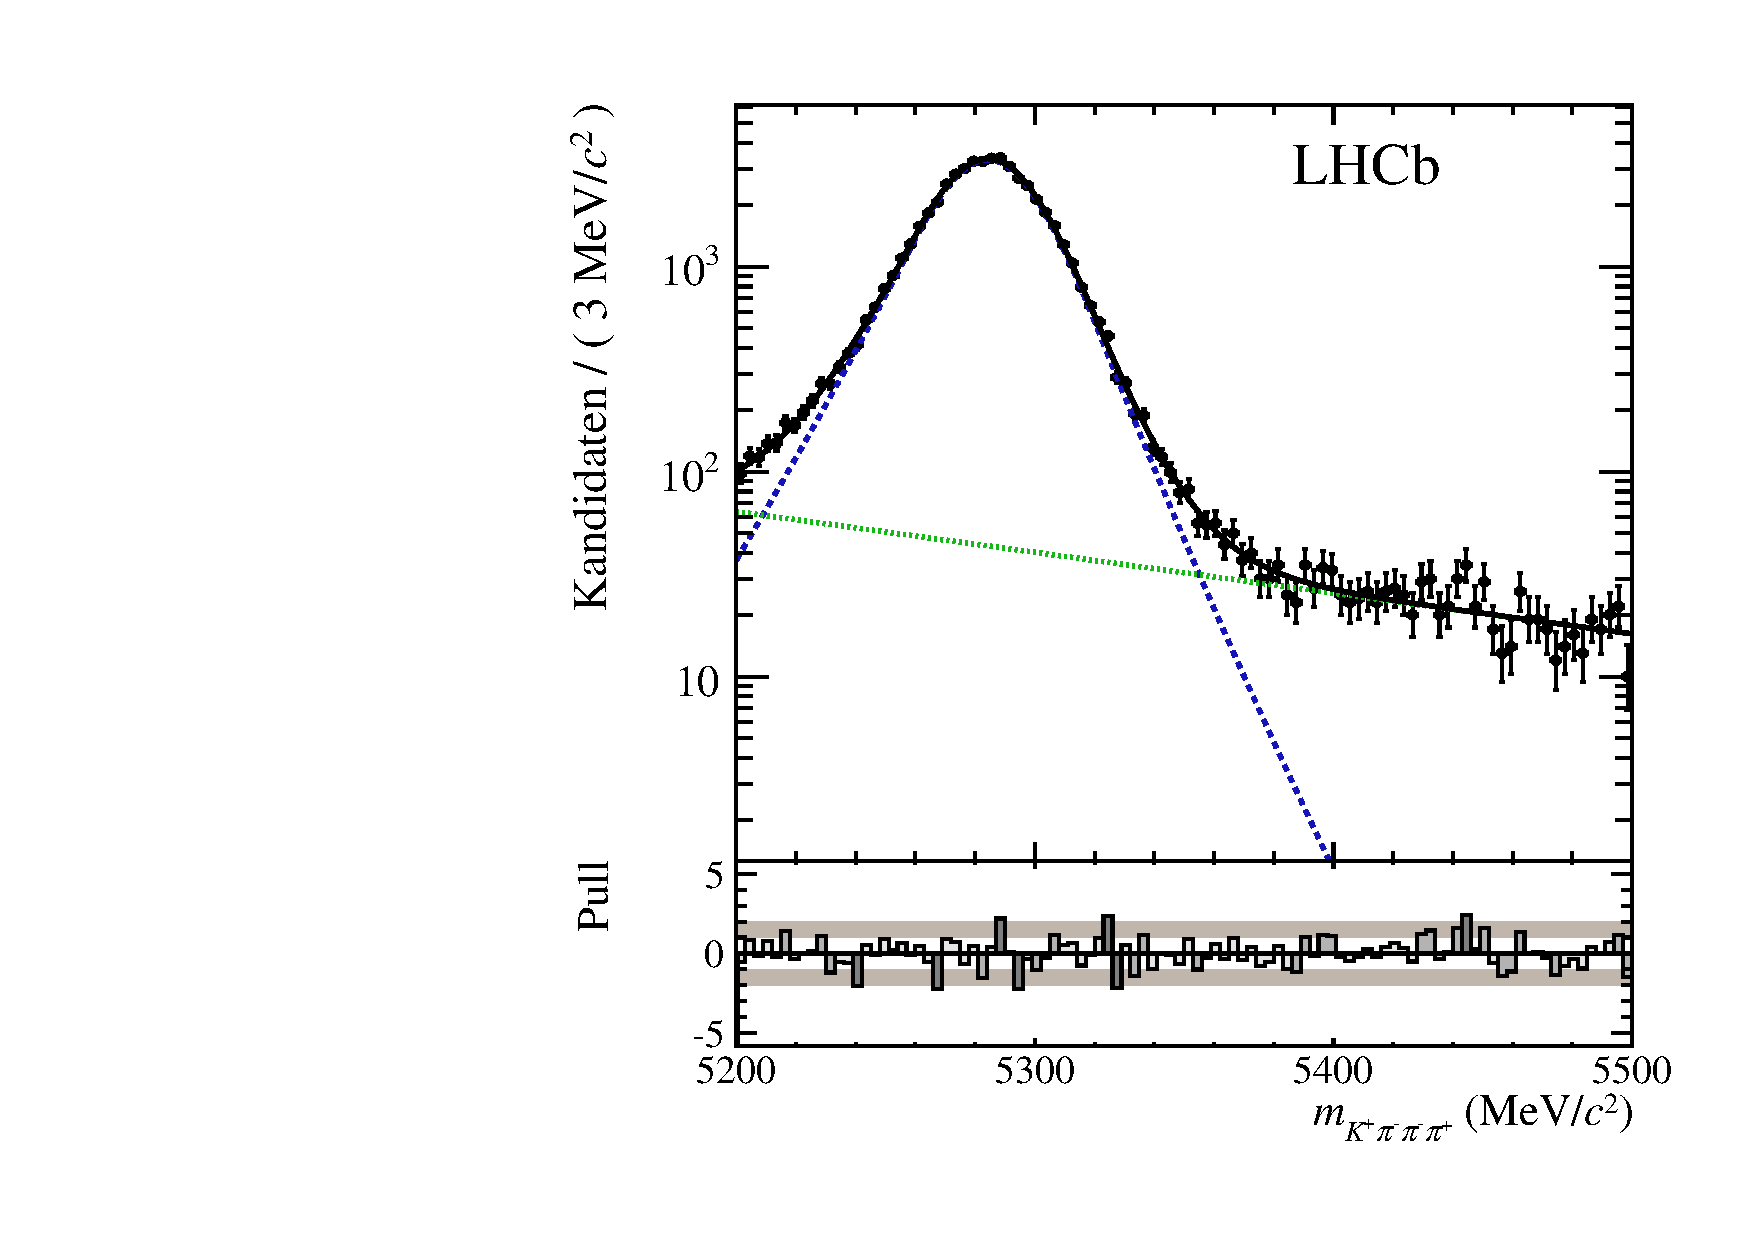
\includegraphics[width=0.45\textwidth]{fig/mass_OS_2011.pdf}
		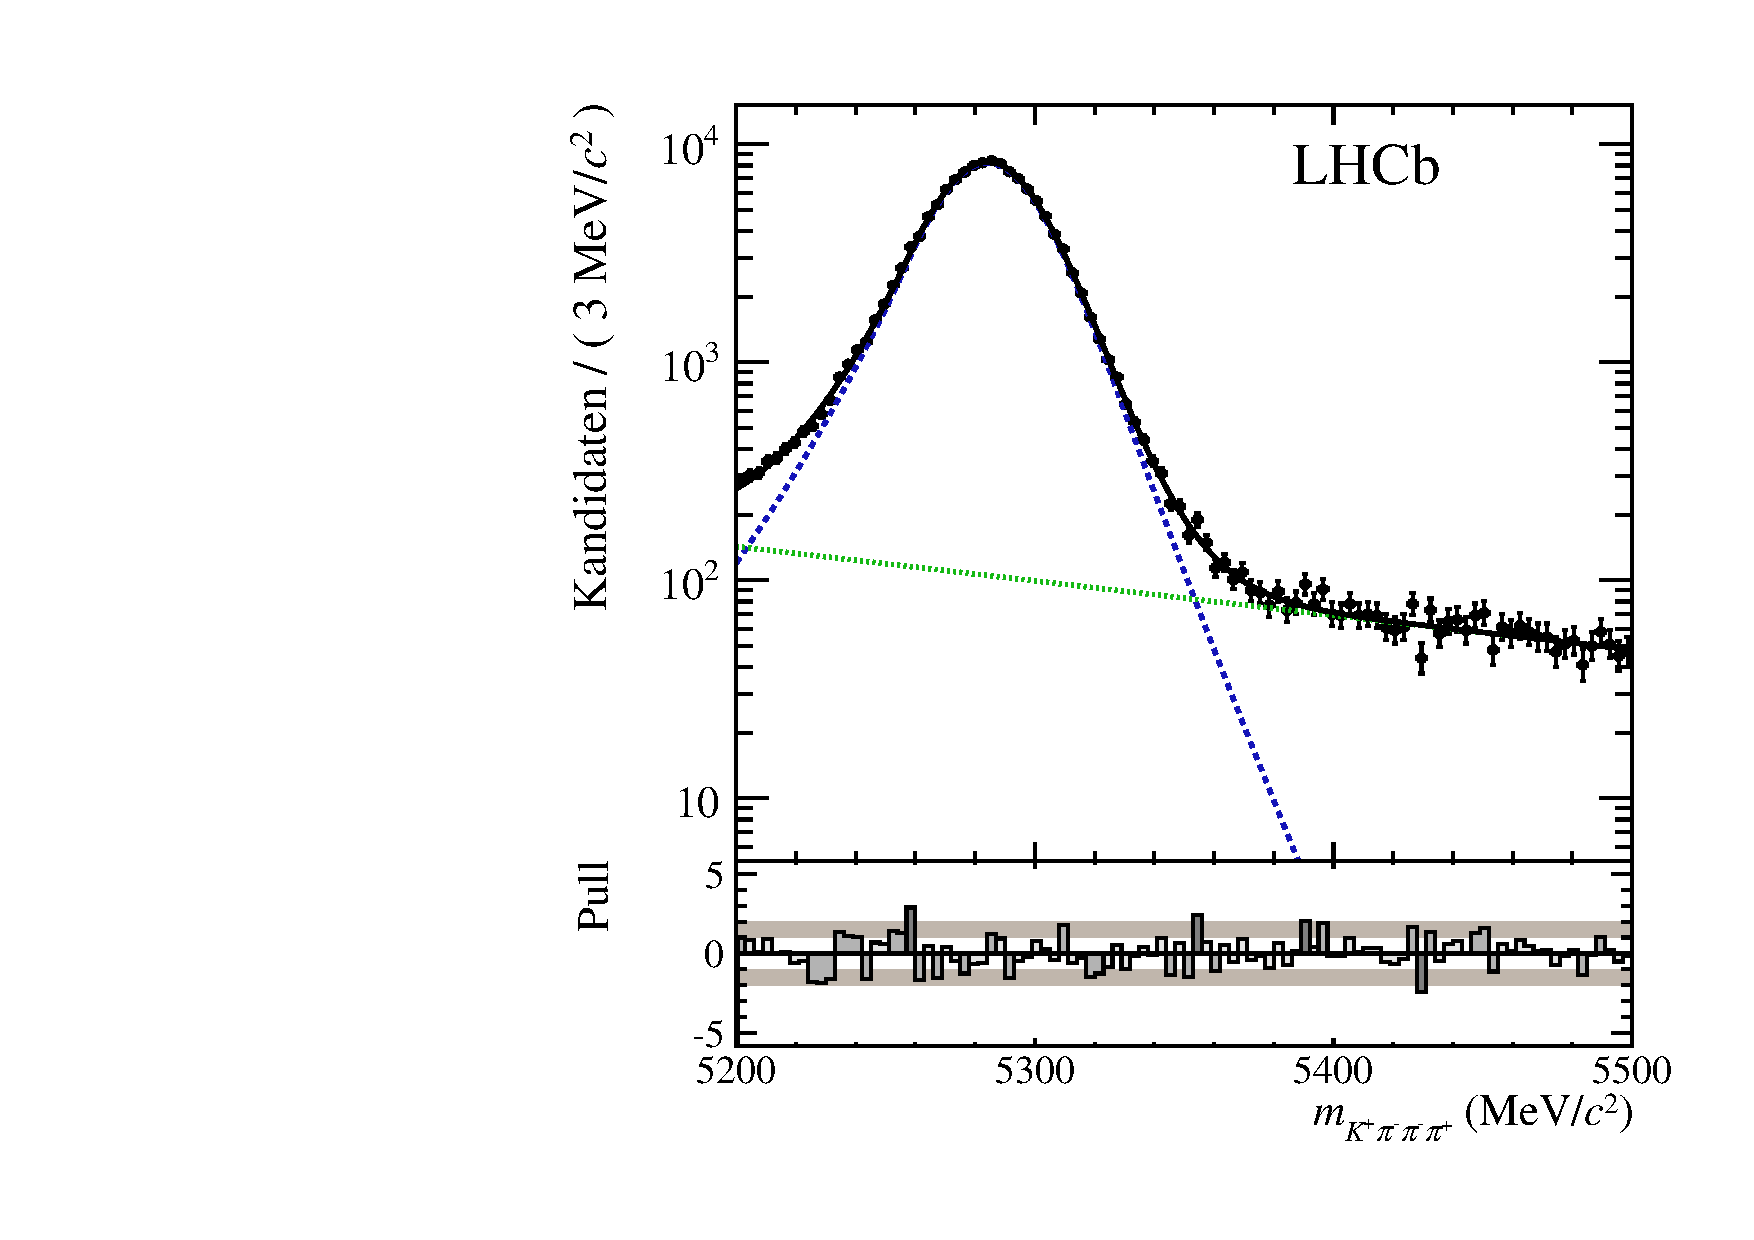
\includegraphics[width=0.45\textwidth]{fig/mass_OS_2012.pdf}
	\caption{Massenfit der \Bz-Mesonen für den \lhcb-Datensatz des Jahres \num{2011} (links) und \num{2012} (rechts) bei Signalkandidaten, die mit der OS Standard Kombination getaggt wurden. Im unteren Bereich der Plots ist die Abweichung der Datenpunkte von der angepassten Funktion in Einheiten der Standardabweichung gezeigt.}
	\label{fig:dmd_mass} 
\end{figure}
\begin{figure}[htbp]
	\centering
		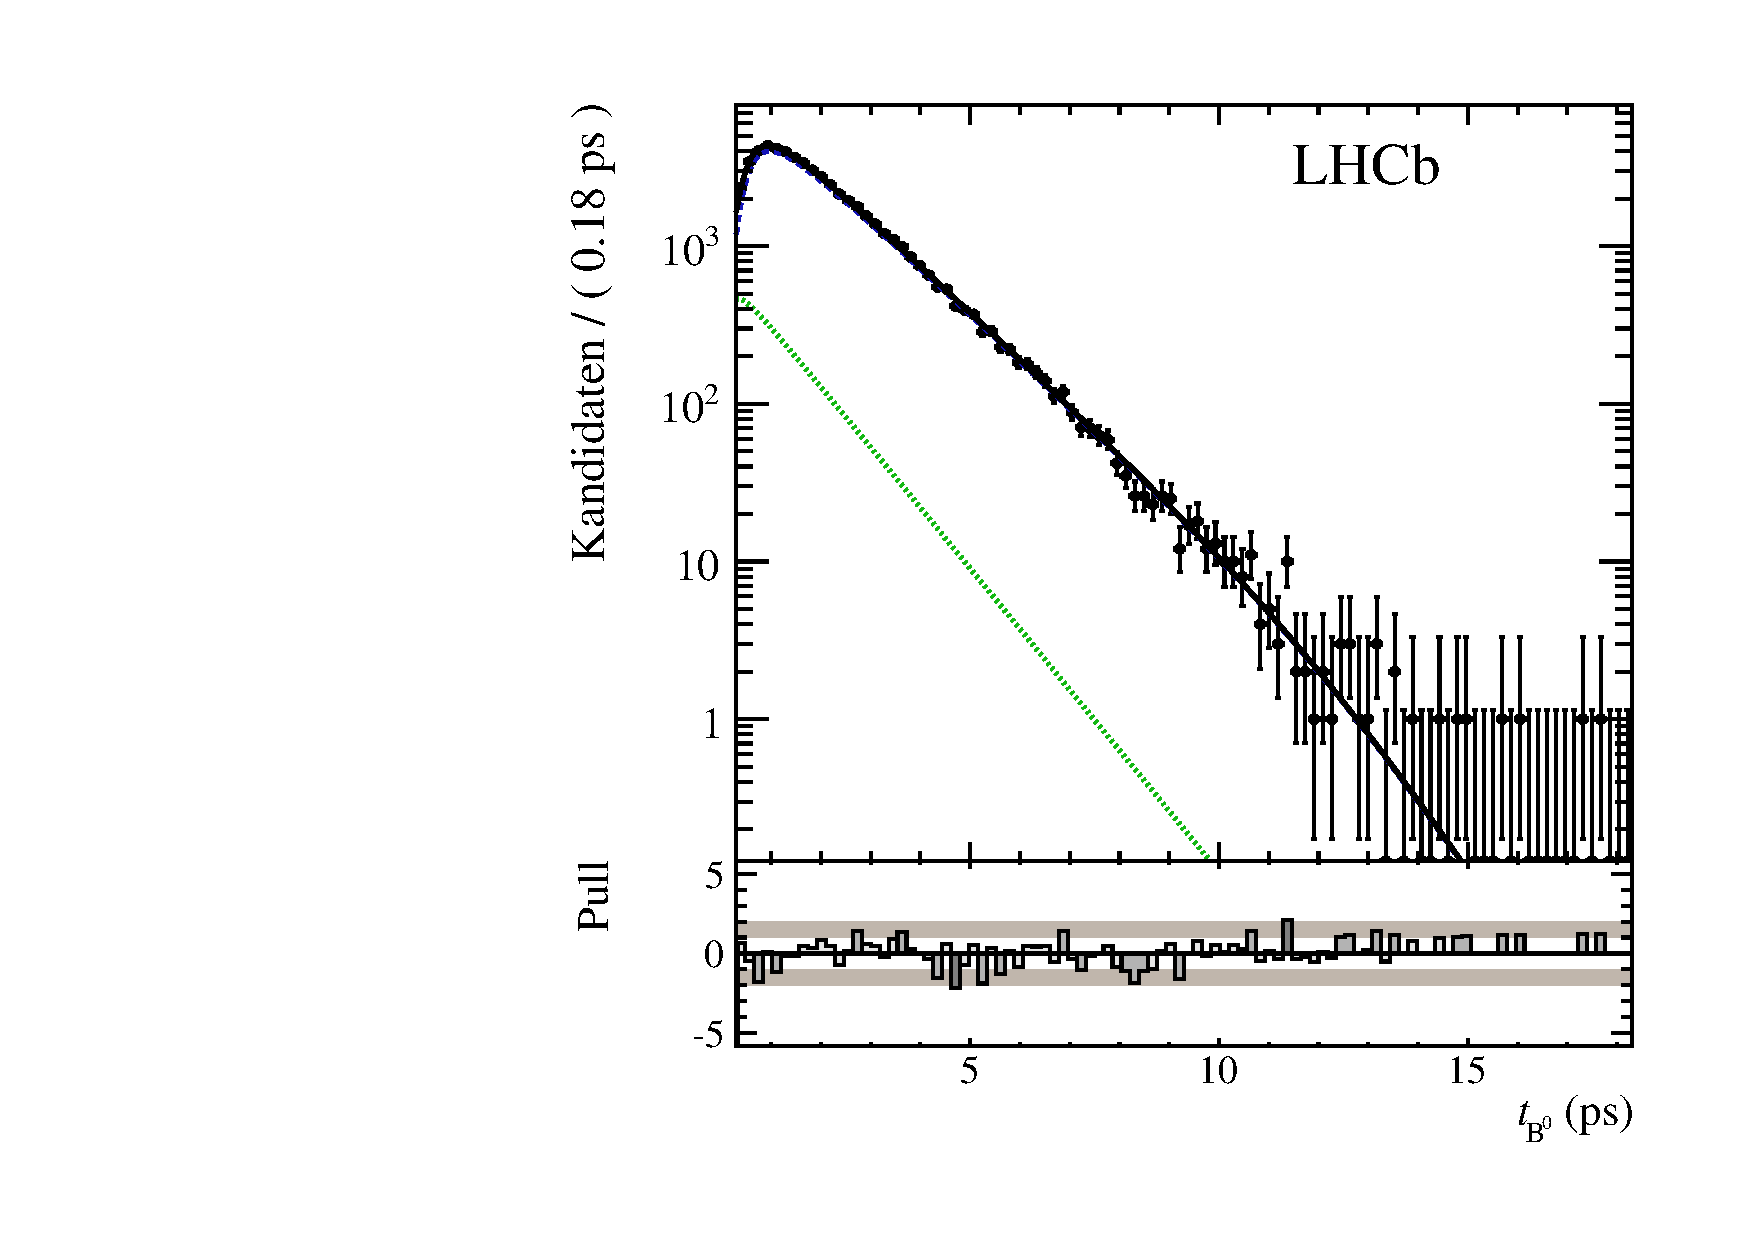
\includegraphics[width=0.45\textwidth]{fig/time_OS_2011.pdf}
		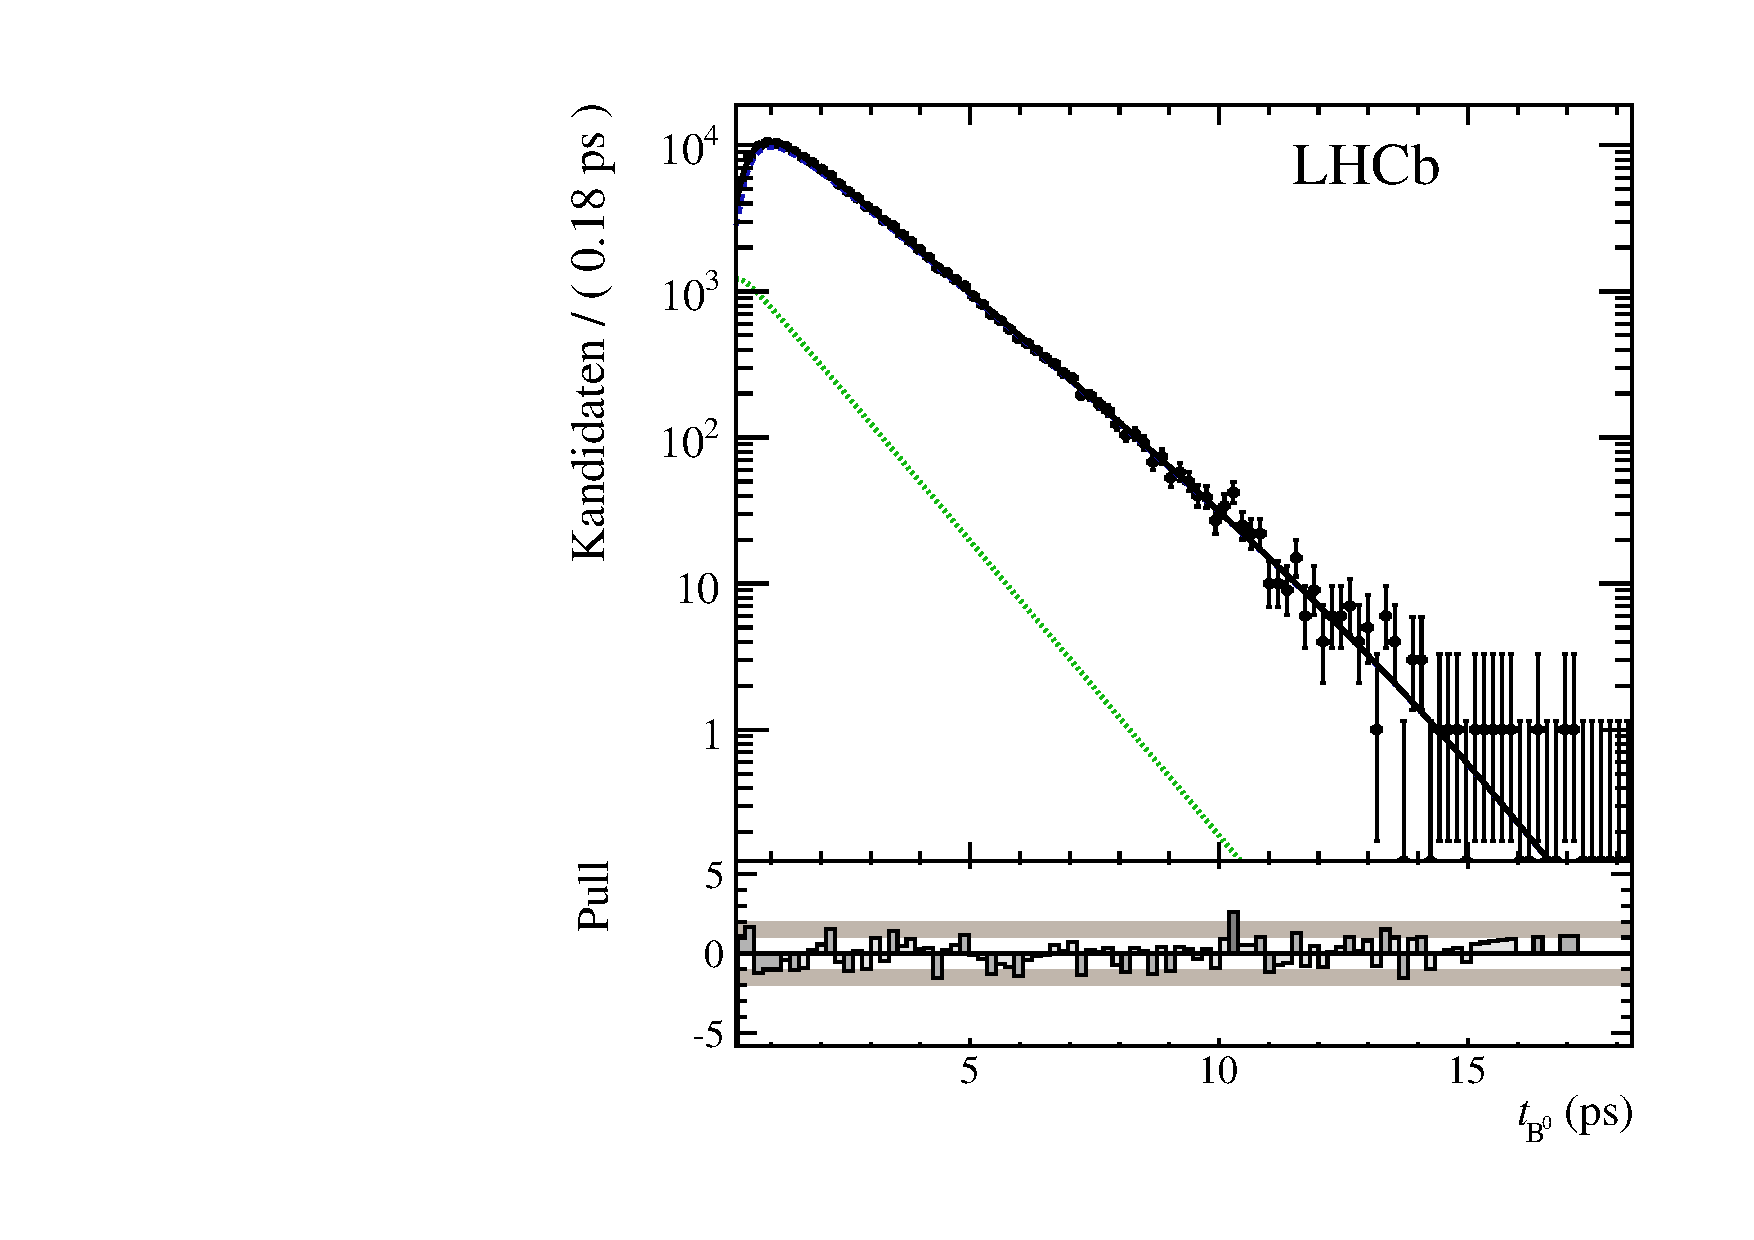
\includegraphics[width=0.45\textwidth]{fig/time_OS_2012.pdf}
	\caption{Lebenszeitfit der \Bz-Mesonen für den \lhcb-Datensatz des Jahres \num{2011} (links) und \num{2012} (rechts) bei Signalkandidaten, die mit der OS Standard Kombination getaggt wurden. Im unteren Bereich der Plots ist die Abweichung der Datenpunkte von der angepassten Funktion in Einheiten der Standardabweichung gezeigt.}
	\label{fig:dmd_time} 
\end{figure} 
\begin{figure}[htbp]
	\centering
		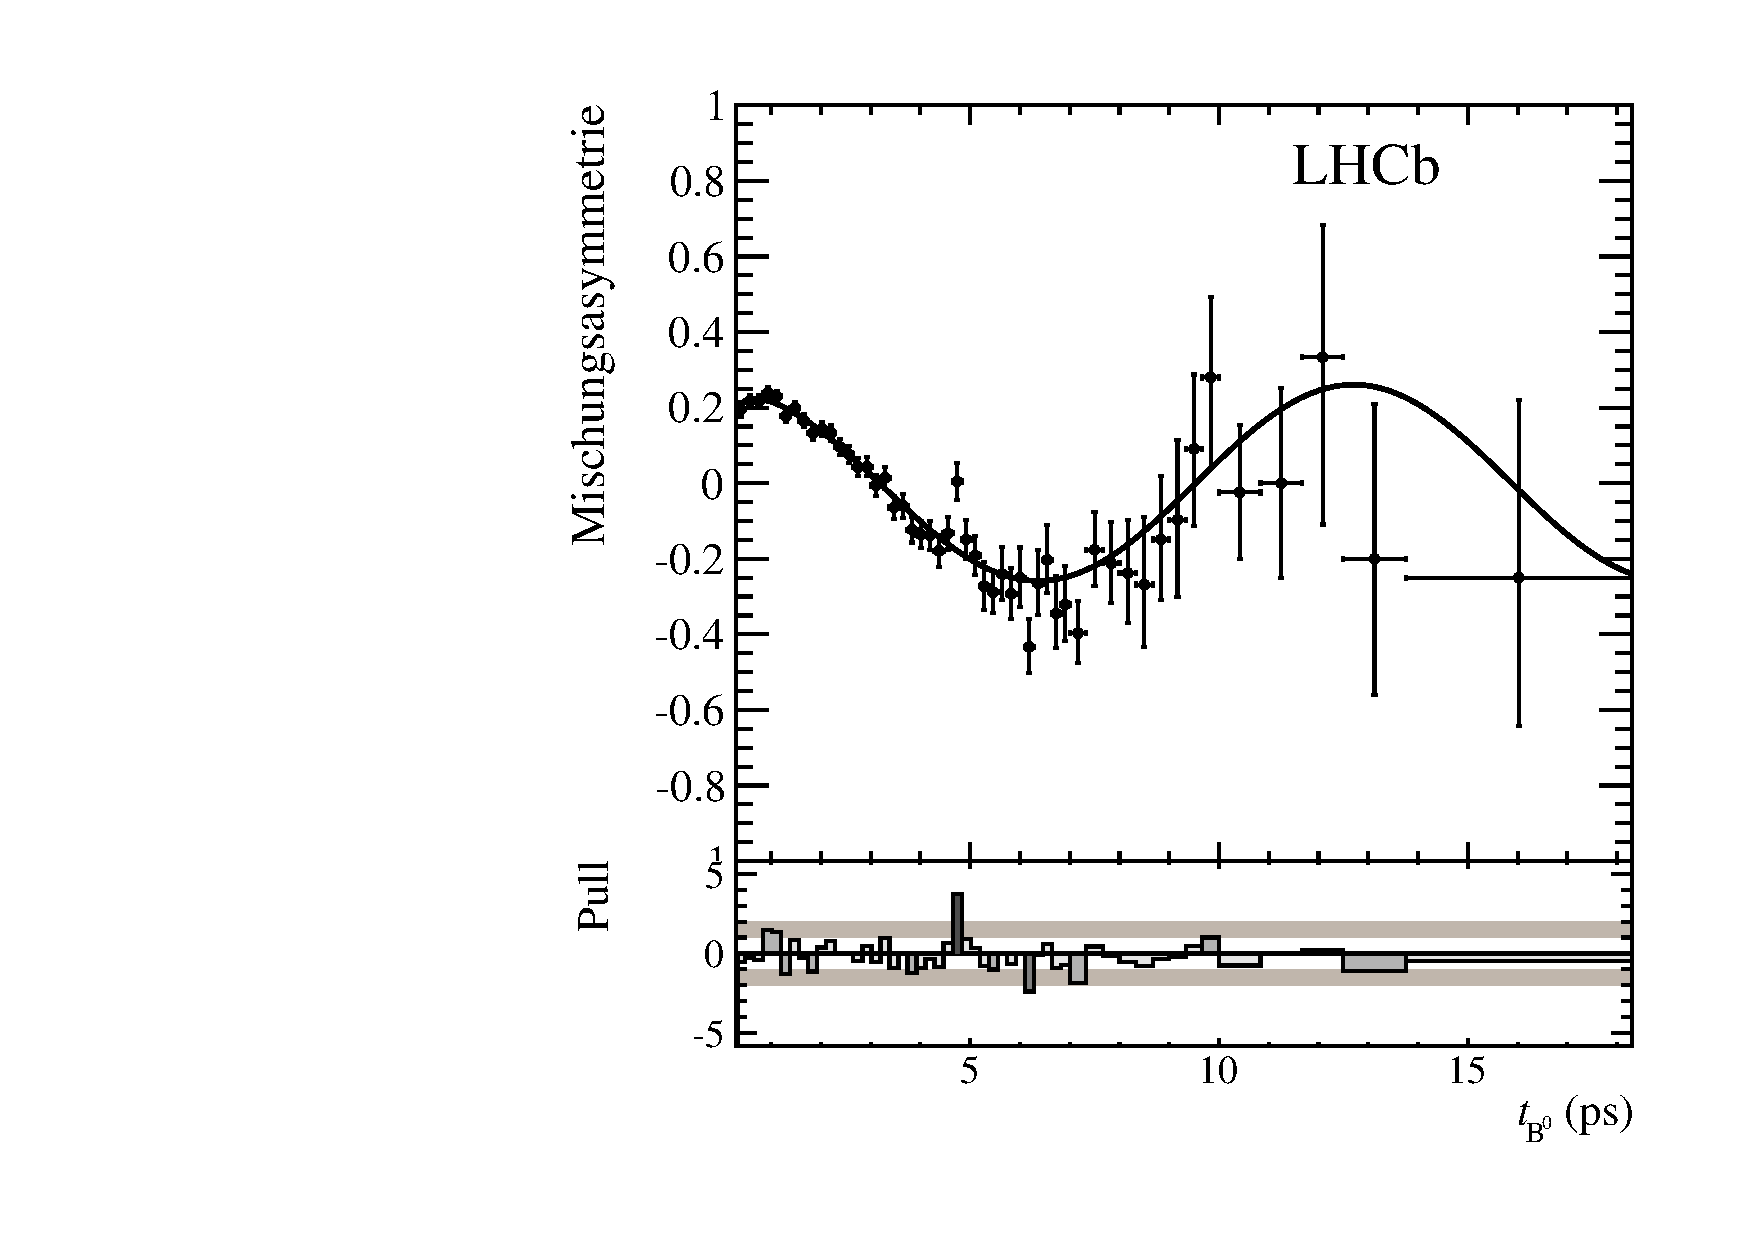
\includegraphics[width=0.45\textwidth]{fig/asymmetry_OS_2011.pdf}
		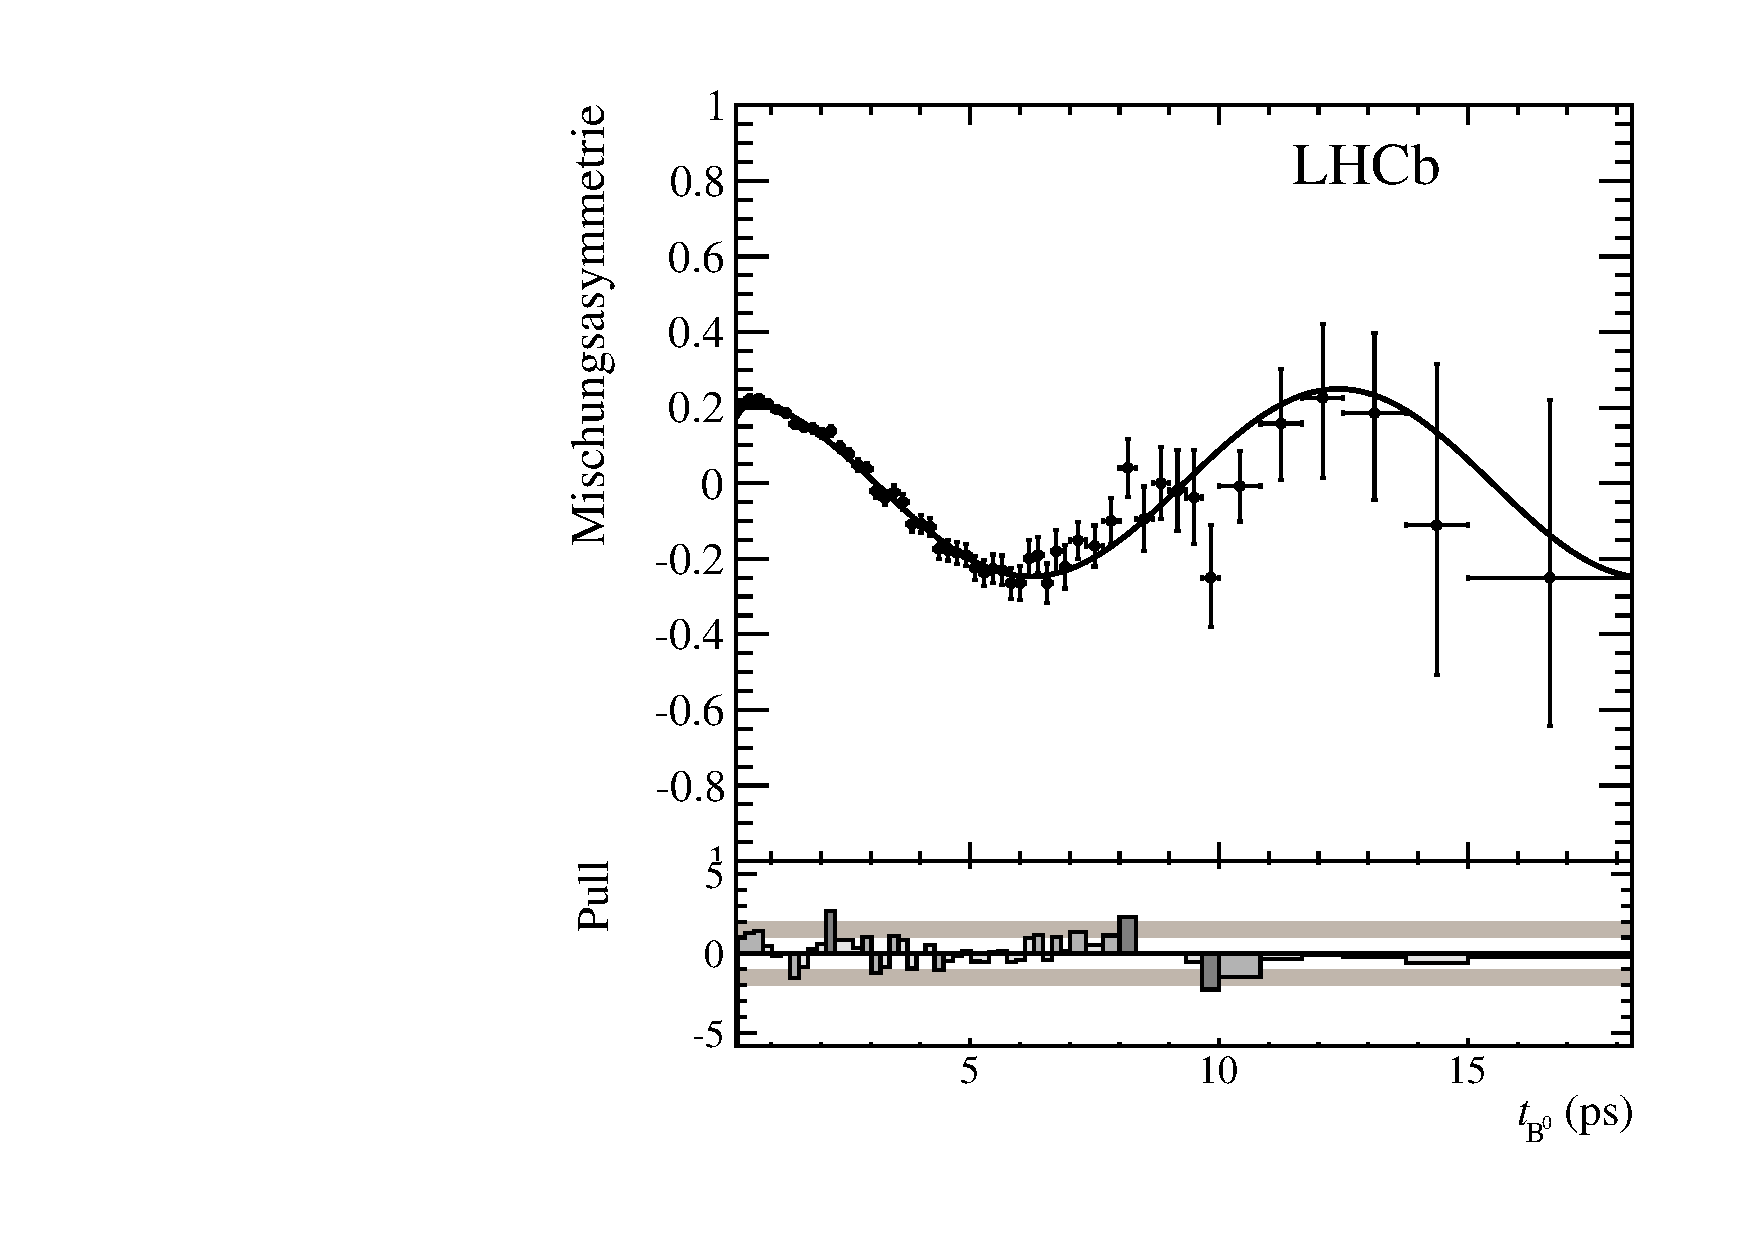
\includegraphics[width=0.45\textwidth]{fig/asymmetry_OS_2012.pdf}
	\caption{Mischungsasymmetrie \eqref{eq:mischung} der \Bz-Mesonen für den \lhcb-Datensatz des Jahres \num{2011} (links) und \num{2012} (rechts) bei Signalkandidaten, die mit der OS Standard Kombination getaggt wurden. Im unteren Bereich der Plots ist die Abweichung der Datenpunkte von der angepassten Funktion in Einheiten der Standardabweichung gezeigt.}
	\label{fig:dmd_asymmetry} 
\end{figure} 
Die statistischen Unsicherheiten auf \dmd sind unbeeinflusst von der Addition des unbekannten Offsets und sollen daher an dieser Stelle mit einer vorherigen Messung  auf dem Datensatz von \num{2011} \cite{dmd_messung} verglichen werden. Bei dieser wurden zur Bestimmung von \dmd die Kombination der Standard OS Kombination mit dem SS Pion Tagger verwendet. Diese sollen an dieser Stelle mit den statistischen Unsicherheiten $\sigma_\text{stat}$ bei einer Messung nur mit der Standard OS Kombination verglichen werden, da bereits hier aufgrund der hohen Statistik für das Jahr \num{2012} zu erwarten ist, dass die statistische Unsicherheit kleiner ist. Für diesen Vergleich sind in Tabelle \ref{tab:Reinheit} zunächst die getaggten Signal und Untergrundkandidaten zu sehen, sowie die sich daraus ergebende Reinheit $\frac{N_\text{Sig}}{N_\text{Bkg}}$.
\begin{table}[htbp]
	\centering
	\caption{Anzahl an Signal- und Untergrundkandidaten aus der \dmd-Messung aus \cite{dmd_messung} und der hier vorgestellten Analyse. Dabei ist zu beachten, dass in der hier vorgestellten Analyse nur die Standard OS Kombination verwendet wurde, während diese zuvor zusätzlich mit dem SS Pion Tagger kombiniert wurde.}
	\label{tab:Reinheit}
	\begin{tabular}{ccccc}
	\toprule
         			&\lhcb Analyse & \multicolumn{2}{c}{aktuelle Analyse} \\  
        Jahr der Datennahme & \num{2011}	 & \num{2011} & \num{2012} \\ 
        \midrule
       $N_\text{Sig}$	& $88200\pm500$ & $53305\pm242$ & $133075\pm^{381}_{380}$ \\ 
       $N_\text{Bkg}$	& $7170\pm^{350}_{390}$& $3470\pm^{94}_{93}$ & $8712\pm143$ \\ 
       \midrule
       $\frac{N_\text{Sig}}{N_\text{Bkg}}$ & $12{,}3\pm^{0{,}6}_{0{,}7}$ & $15{,}4\pm0{,}4$ & $15{,}3\pm0{,}3$  \\ 
       \bottomrule
	\end{tabular}
\end{table}
Bei dieser erkennt man, dass die aktuelle Selektion für beide Jahre bessere Ergebnisse für die Reinheit liefert. Die statistische Unsicherheit in der aktuellen Analyse ist für die Daten des Jahres \num{2011} größer, weil hier nur die OS Kombination verwendet wurde. Die Analyse der von der OS Kombination getaggten Signalkandidaten in den \num{2012} aufgenommenen Daten sollte allerdings bereits zu einer kleineren statistischen Unsicherheit führen. Der Vergleich der Unsicherheiten ist in Tabelle \ref{tab:statFehler} zu sehen und man erkennt, dass die Erwartungen bezüglich einer statistisch größeren Genauigkeit bestätigt werden.
\begin{table}[htbp]
	\centering
	\caption{Statistische Unsicherheit $\sigma_\text{stat}$ auf die Größe \dmd. In der Analyse aus \num{2012} \cite{dmd_messung} wurde dieser extrahiert aus einer Kombination des SS Pion Taggers mit der OS Kombination. In der aktuellen Analyse wurde nur die OS Kombination verwendet.}
	\label{tab:statFehler} 
	\begin{tabular}{c|c|cccc}
	\toprule
         			&\lhcb Analyse & \multicolumn{3}{c}{aktuelle Analyse} \\  
        Jahr der Datennahme & \num{2011}	 & \num{2011} & \num{2012} & \num{2011}\&\num{2012}\\ 
        \midrule
       $\sigma_\text{stat}$	& \num{0{,}0061} & \num{0{,}0082} & \num{0{,}0055} & \num{0{,}0045} \\ 
       \bottomrule
	\end{tabular}
\end{table}

\section{Alternative Kalibrierung der OS Kombination}

Im Folgenden soll das in Abschnitt \ref{sec:kalibrierungDaten} erläuterte zweite Verfahren zur Kalibrierung des Flavour Taggings auf die OS Kombination angewendet werden. Dabei wird an dieser Stelle wegen der größeren Statistik der Datensatz aus dem Jahr \num{2012} verwendet. Es werden insgesamt \num{32} Kategorien der Wahrscheinlichkeit $P_\text{tag}(\bquarkbar)$ so gewählt, dass alle etwa die gleiche Statistik enthalten. Dabei gibt es kleine Unterschiede für die Kategorien für $P_\text{tag}(\bquarkbar)>0{,}5$ und $P_\text{tag}(\bquarkbar)<0{,}5$, da bei der Kategorisierung bei $P_\text{tag}(\bquarkbar)=0{,}5$ getrennt werden musste, um weiterhin zwischen \Bz- und \Bzb-Mesonen zu unterscheiden. In den Abbildungen \ref{fig:PBgetrennt1} und \ref{fig:PBgetrennt2} sind nun zunächst die Ergebnisse der linearen Kalibrierungen getrennt in den Bereichen $0<P_\text{tag}(\bquarkbar)<0{,}5$ und $0{,}5<P_\text{tag}(\bquarkbar)<1$ zu sehen. In Tabelle \ref{tab:PBgetrennt} sind die zugehörigen Ergebnisse dargestellt. Außerdem sieht man dort die Kalibrationsparameter $\Delta p_0$ und $\Delta p_1$, die die Taggingasymmetrie beschreiben. Diese berechnen sich hier nach
\begin{equation}
\Delta p_0=\left(1-p_0\right)-\overline{p_0}\hspace{1cm}\text{ und }\hspace{1cm}\Delta p_1=p_0-\overline{p_0}.
\end{equation}
Für die Zentralwerte $\widetilde{p_0}$ und $\widetilde{p_1}$ gilt
\begin{equation}
\widetilde{p_0}=\frac{\left(1-p_0\right)+\overline{p_0}}{2}\hspace{1cm}\text{ und }\hspace{1cm}\widetilde{p_1}=\frac{p_0+\overline{p_0}}{2}.
\end{equation}
 \begin{figure}[htbp]
	\centering
		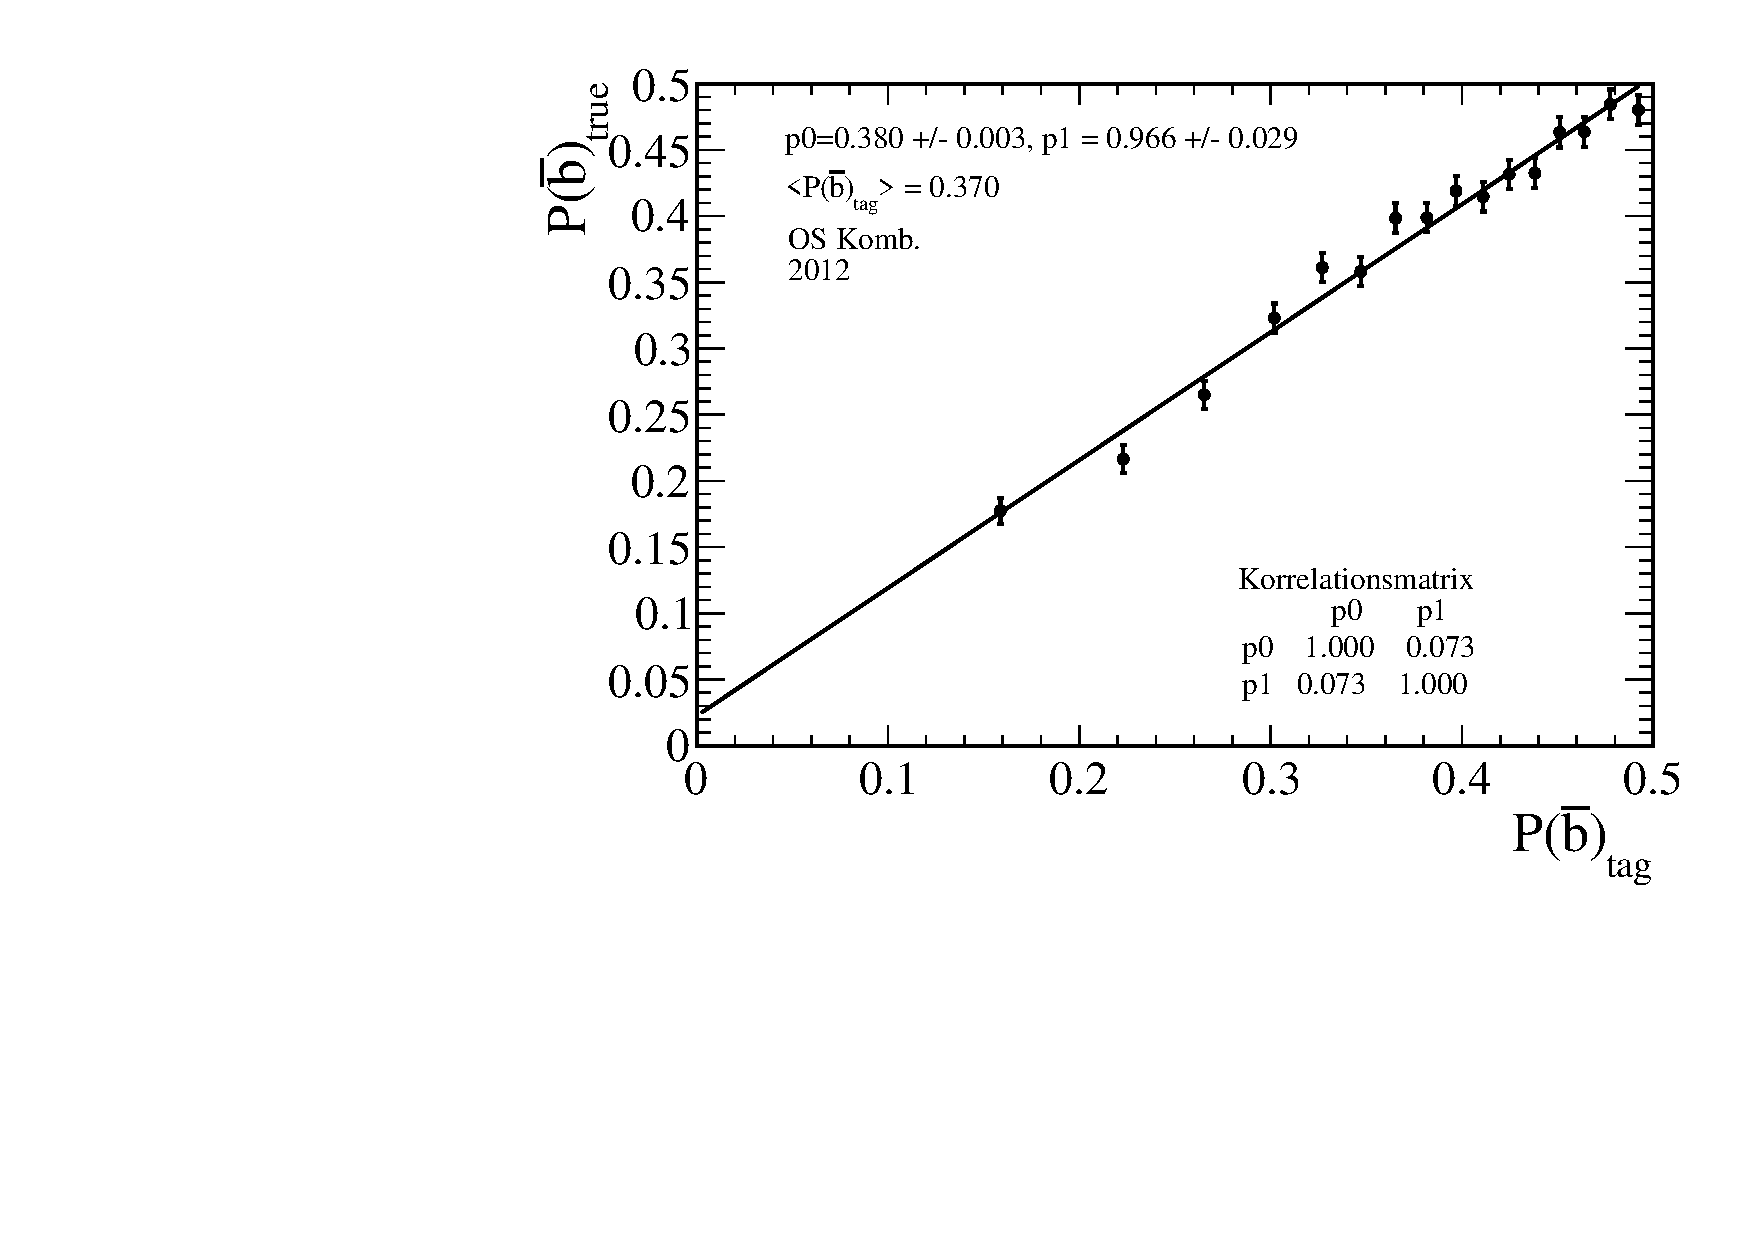
\includegraphics[width=0.75\textwidth]{fig/calibration_Bbar.pdf}
	\caption{Kalibrierung der OS Standard Kombination mit Wahrscheinlichkeiten \mbox{$P(\bquarkbar)<0{,}5$} für \Bzb-Mesonen.}
	\label{fig:PBgetrennt1} 
\end{figure} 
 \begin{figure}[htbp]
	\centering
		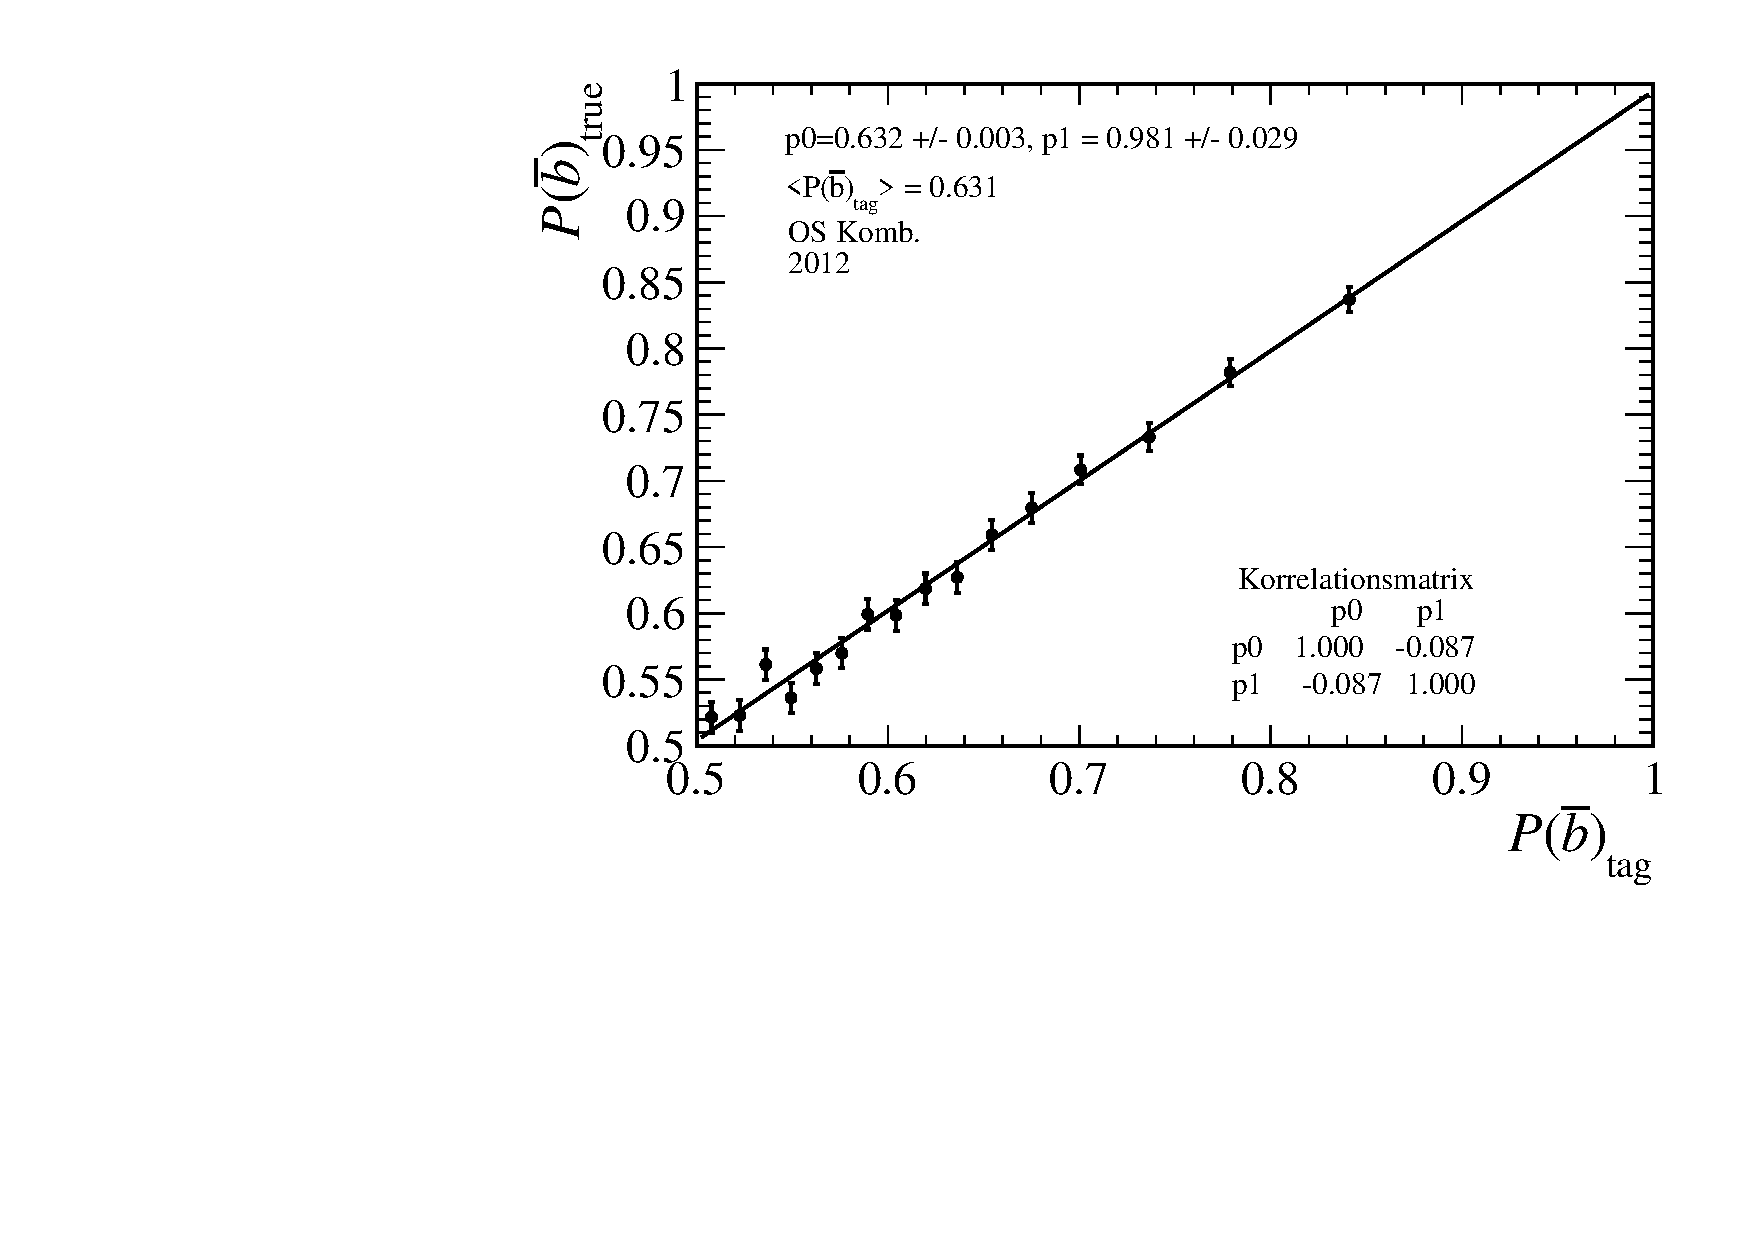
\includegraphics[width=0.75\textwidth]{fig/calibration_B.pdf}
	\caption{Kalibrierung der OS Standard Kombination mit Wahrscheinlichkeiten \mbox{$P(\bquarkbar)>0{,}5$} für \Bz-Mesonen.}
	\label{fig:PBgetrennt2} 
\end{figure} 
\begin{table}[htbp]
	\centering
	\caption{Ergebnisse der linearen Kalibrierung der OS Standard Kombination mit Wahrscheinlichkeiten $P(\bquarkbar)$. Zum Vergleich die Ergebnisse der $(\eta,\omega)$-Kalibrierung.}
	\label{tab:PBgetrennt} 
	\begin{tabular}{c|ccc}
	\toprule
	 & $0<P_\text{tag}(\bquarkbar)<0{,}5$ & $0{,}5<P_\text{tag}(\bquarkbar)<1$ & $(\eta,\omega)$-Kalibrierung \\ 
	 \midrule
      $p_0$/$\overline{p_0}$  & $0{,}380\pm0{,}003$ & $0{,}632\pm0{,}003$ & - \\  
      $p_1$/$\overline{p_1}$ & $0{,}966\pm0{,}029$ & $0{,}981\pm0{,}029$ & - \\
      $\widetilde{p_0}$ & \multicolumn{2}{c}{$0{,}374\pm0{,}002$} &  $0{,}376\pm0{,}002$ \\
      $\widetilde{p_1}$ &  \multicolumn{2}{c}{$0{,}974\pm0{,}021$} &  $0{,}981\pm0{,}020$ \\
      $\Delta p_0$ & \multicolumn{2}{c}{$-0{,}012\pm0{,}004$} &  $0{,}018\pm0{,}003$ \\
      $\Delta p_1$ & \multicolumn{2}{c}{$-0{,}015\pm0{,}041$} &  $0{,}069\pm0{,}029$ \\ 
      \bottomrule
	\end{tabular}
\end{table}
Man sieht, dass die Ergebnisse für die Taggingasymmetrien dabei eindeutig von den Ergebnissen der Gesamtparametrisierung aus der $(\eta,\omega)$-Kalibrierung abweichen. Dies ilässt sich erklären, da die Taggingasymmetrien für die \enquote{echten} initialen \B-Mesonen definiert sind. Bei der Unterscheidung für die hier gezeigte Kalibrierung, steht jedoch nur die fehlerbehaftete Tagentscheidung zur Verfügung.\\ 
Dies lässt sich auf Monte-Carlo Daten bestätigen, wo der anfängliche Flavour der \B-Mesonen bekannt ist. In Tabelle \ref{tab:mcgetrennt} wurde dazu zunächst eine komplette Kalibrierung auf Monte-Carlo mit einem Zeitfit durchgeführt. Aus dieser Kalibrierung erhält man die Parameter $\widetilde{p_0}$, $\widetilde{p_1}$, $\Delta p_0$ und $\Delta p_1$. Außerdem lässt sich, auch auf Monte-Carlo, die Kalibrierung getrennt nach der Tagentscheidung, für getaggte \Bz- und \Bzb-Mesonen durchführen, um so die Parameter $p_0$, $\overline{p_0}$, $p_1$ und $\overline{p_1}$ zu erhalten. Dabei sieht man wiederum die qualitativ gleichen Unterschiede wie in Tabelle \ref{tab:PBgetrennt} auf Daten. Als weitere Möglichkeit lässt sich auf Monte-Carlo nun allerdings auch nach dem in Abschnitt \ref{sec:mckalibrierung} beschriebenen Verfahren für \Bz- und \Bzb-Mesonen getrennt kalibrieren, wobei allerdings nicht nach der Tagentscheidung, sondern dem \enquote{wahren} Anfangszustand unterschieden wird.
\begin{table}[htbp]
	\centering
	\small
	\caption{Vergleich der linearen Kalibrierungsparameter auf Monte-Carlo bei der Beschreibung der Taggingasymmetrie. In der ersten Zeile ist die Größe angegeben, nach der für die Kalibrierung getrennt wurde.}
	\label{tab:mcgetrennt} 
	\begin{tabular}{c|ccccc}
	\toprule
	 & \multicolumn{2}{c}{Tag $d$} & \multicolumn{2}{c}{\enquote{wahrer} Flavour} & Gesamtfit \\
	 & \Bzb & \Bz & \Bzb & \Bz & \Bzb \& \Bz \\ 
	 \midrule
      $p_0$/$\overline{p_0}$  & $0{,}353\pm0{,}011$ & $0{,}349\pm0{,}011$ & $0{,}348\pm0{,}007$ & $0{,}353\pm0{,}007$ & - \\  
      $p_1$/$\overline{p_1}$ & $0{,}933\pm0{,}116$ & $0{,}772\pm0{,}122$ & $0{,}876\pm0{,}077$ & $0{,}916\pm0{,}078$ & - \\
      $\widetilde{p_0}$ & \multicolumn{2}{c}{$0{,}351\pm0{,}008$} & \multicolumn{2}{c}{$0{,}351\pm0{,}005$} &  $0{,}350\pm0{,}008$ \\
      $\widetilde{p_1}$ &  \multicolumn{2}{c}{$0{,}853\pm0{,}084$} & \multicolumn{2}{c}{$0{,}896\pm0{,}054$} & $0{,}828\pm0{,}082$ \\
      $\Delta p_0$ & \multicolumn{2}{c}{$-0{,}004\pm0{,}015$} & \multicolumn{2}{c}{$0{,}005\pm0{,}010$} & $0{,}005\pm0{,}009$ \\
      $\Delta p_1$ & \multicolumn{2}{c}{$-0{,}161\pm0{,}168$} & \multicolumn{2}{c}{$0{,}040\pm0{,}110$} & $0{,}029\pm0{,}052$ \\ 
      \bottomrule
	\end{tabular}
\end{table}
Vergleicht man nun die sich ergebenden Taggingasymmetrien zwischen den beiden getrennten Kalibrierungen jeweils mit der Kalibrierung aus dem Gesamtfit, sieht man, dass die Parameter für die Trennung nach \enquote{wahrem} Produktionsflavour eine gute Übereinstimmung zeigen, während bei der Trennung nach der Tagentscheidung $d$ hier ähnliche Effekte wie zuvor zu beobachten sind.\\
Vorteil der hier vorgestellten Methode wäre eine gleiche Verwendung der Wahrscheinlichkeiten wie die Flavour-Tagging-Software. Diese müsste zur weiteren Verwendung nicht in mistag-Wahrscheinlichkeiten $\eta$ umgerechnet werden. Weiter ist die Trennung zwischen getaggten \Bz- und \Bzb-Mesonen sehr einfach durch einen Schnitt bei $P(\bquarkbar)=0{,}5$ realisierbar. Nachteil ist, dass die Parameter der Taggingasymmetrie $\Delta p_0$ und $\Delta p_1$ nicht durch die einfache Trennung nach dem tag ermittelbar sind. 
 
